%% 
%% Copyright 2007, 2008, 2009 Elsevier Ltd
%% 
%% This file is part of the 'Elsarticle Bundle'.
%% ---------------------------------------------
%% 
%% It may be distributed under the conditions of the LaTeX Project Public
%% License, either version 1.2 of this license or (at your option) any
%% later version.  The latest version of this license is in
%%    http://www.latex-project.org/lppl.txt
%% and version 1.2 or later is part of all distributions of LaTeX
%% version 1999/12/01 or later.
%% 
%% The list of all files belonging to the 'Elsarticle Bundle' is
%% given in the file `manifest.txt'.
%% 
%% Template article for Elsevier's document class `elsarticle'
%% with harvard style bibliographic references
%% SP 2008/03/01

%\documentclass[preprint,12pt,authoryear]{elsarticle}  %default in the template
%\documentclass[preprint,10pt,authoryear]{elsarticle}

%% Use the option review to obtain double line spacing
%% \documentclass[authoryear,preprint,review,12pt]{elsarticle}

%% Use the options 1p,twocolumn; 3p; 3p,twocolumn; 5p; or 5p,twocolumn
%% for a journal layout:
%% \documentclass[final,1p,times,authoryear]{elsarticle}
%% \documentclass[final,1p,times,twocolumn,authoryear]{elsarticle}
 \documentclass[final,3p,times,authoryear]{elsarticle}
%% \documentclass[final,3p,times,twocolumn,authoryear]{elsarticle}
%% \documentclass[final,5p,times,authoryear]{elsarticle}
%% \documentclass[final,5p,times,twocolumn,authoryear]{elsarticle}

%% For including figures, graphicx.sty has been loaded in
%% elsarticle.cls. If you prefer to use the old commands
%% please give \usepackage{epsfig}

%% The amssymb package provides various useful mathematical symbols
\usepackage{amssymb}
%% The amsthm package provides extended theorem environments
 \usepackage{amsthm}
 \usepackage{amsmath}
 \usepackage{color}
 \usepackage{amsmath}
\usepackage{siunitx}


\usepackage{framed} % Framing content
\usepackage{multicol} % Multiple columns environment
\usepackage{nomencl} % Nomenclature package
\makenomenclature
%\setlength{\nomitemsep}{-\parskip} % Baseline skip between items
\setlength{\nomitemsep}{0.01cm}
\renewcommand*\nompreamble{\begin{multicols}{2}}
\renewcommand*\nompostamble{\end{multicols}}


\usepackage{subfig}
\usepackage{graphicx}

%% The lineno packages adds line numbers. Start line numbering with
%% \begin{linenumbers}, end it with \end{linenumbers}. Or switch it on
%% for the whole article with \linenumbers.
%% \usepackage{lineno}

\journal{Urban Climate}

\begin{document}

\begin{frontmatter}

%% Title, authors and addresses

%% use the tnoteref command within \title for footnotes;
%% use the tnotetext command for theassociated footnote;
%% use the fnref command within \author or \address for footnotes;
%% use the fntext command for theassociated footnote;
%% use the corref command within \author for corresponding author footnotes;
%% use the cortext command for theassociated footnote;
%% use the ead command for the email address,
%% and the form \ead[url] for the home page:
%% \title{Title\tnoteref{label1}}
%% \tnotetext[label1]{}
%% \author{Name\corref{cor1}\fnref{label2}}
%% \ead{email address}
%% \ead[url]{home page}
%% \fntext[label2]{}
%% \cortext[cor1]{}
%% \address{Address\fnref{label3}}
%% \fntext[label3]{}

\title{Development of the VTUF-3D v1.0 urban micro-climate model to support assessments of urban vegetation influences on human thermal comfort}


%% use optional labels to link authors explicitly to addresses:
\author[monash,melb,crc]{Kerry~A.~Nice\corref{cor1}}
\ead{mothlight@fastmail.fm}
\author[monash,crc]{Andrew~M.~Coutts}
\author[monash,crc]{Nigel~J.~Tapper}
\cortext[cor1]{Principal corresponding author}
\address[monash]{School of Earth, Atmosphere and Environment, Monash University, Clayton, Victoria 3800, Australia}
\address[melb]{Transport, Health, and Urban Design Hub, Faculty of Architecture, Building, and Planning, University of Melbourne, Victoria 3010, Australia}
\address[crc]{Cooperative Research Centre for Water Sensitive Cities, Melbourne, Australia}


\begin{abstract}

With urban areas facing longer duration heat-waves and temperature extremes from climate change and growing urban development, adaptation strategies are needed to protect city residents. Examining the role that increased tree cover and water availability can have on human thermal comfort (HTC) is needed to help guide the development of thermally comfortable cities. To inform planning, modelling tools are needed that provide sufficient resolution to resolve urban influences on HTC and the ability to model important physiological processes of vegetation. To achieve this, a new micro-scale model, VTUF-3D (Vegetated Temperatures of Urban Facets), has been developed using an innovative approach of embedding the functionality of the MAESPA tree process model \citep{Duursma2012}, a model that can model individual trees, vegetation, and soil components, within the TUF-3D \citep{Krayenhoff2007} urban micro-climate model. An innovative tiling approach allows the new model to account for important vegetative physiological processes and shading effects, using configurable templates to allow representation of any type of vegetation or water sensitive design feature. This work enables detailed calculations of surface temperatures ($T_{sfc}$), mean radiant temperature ($T_{mrt}$), and a HTC index, the universal thermal climate index (UTCI), across an urban canyon. This study presents an overview of VTUF-3D. Also presented are two evaluations of VTUF-3D. The first compares modelled surface energy balance fluxes to observations in Preston, Australia \citep{Coutts2007}. The second using spatial and temporal predictions of $T_{mrt}$ and UTCI across two observed street canyons in the City of Melbourne \citep{Coutts2015}. The VTUF-3D model is shown to perform well and is suitable for use to examine critical questions relating to the role of vegetation and water in the urban environment. Using this model, it is now possible to conduct further analysis to quantify the impact each individual tree can have on conditions in urban canyons. Further, the model can help inform the optimal arrangement and quantity of trees to deliver improvements in HTC and be used to generate best practice guidelines for urban greening.


\end{abstract}

\begin{keyword}
micro-climate modelling, urban vegetation, VTUF-3D, human thermal comfort, mean radiant temperature, UTCI
%% keywords here, in the form: keyword \sep keyword

%% PACS codes here, in the form: \PACS code \sep code

%% MSC codes here, in the form: \MSC code \sep code
%% or \MSC[2008] code \sep code (2000 is the default)

\end{keyword}

\end{frontmatter}

\begin{table*}[!t]   
\begin{framed}
\printnomenclature
%%\nomenclature{$A _{canopy}$}{canopy area (m$^{2}$)} 
%\nomenclature{$A _{mm}$}{2-dimensional tree area (mm$^{2}$)} 
%\nomenclature{$A$}{surface area of a sphere of diameter D, of value 0.15m, (=$\pi 0.15^{2}$m$^{2}$)} 
%\nomenclature{$A_{leaf}$}{total leaf area (m$^{2}$)} 
%%\nomenclature{$D_{eff}$}{effective diffusivity of the soil pore space (m$^{2}$s$^{-1}$)} 
%%\nomenclature{$E_{L}$}{leaf level transpiration rate ($\mu$mol m$^{-2}$s$^{-1}$)} 
%%\nomenclature{$E_{i}$}{root water uptake (canopy transpiration) out of layer i (mm)} 
%%\nomenclature{$E_{s}$}{rate of evaporation (mm)} 
%%\nomenclature{$F_{R}$}{cumulative fraction of fine roots to depth z (m)} 
%%\nomenclature{$G_{ws}$}{conductance of water vapour through the soil pore space (m s$^{-1}$)} 
%\nomenclature{$H _{blt}$}{building height (m)} 
%\nomenclature{$H _{crown}$}{crown height (m)} 
%\nomenclature{$H _{trunk}$}{trunk height (m)} 
%\nomenclature{$H$}{tree height (m)}
%\nomenclature{$H_{top}$}{convective sensible heat flux density between canopy air and boundary layer (Wm$^{-2}$)} 
%%\nomenclature{$K\downarrow$}{downward shortwave radiative flux density (Wm$^{-2}$)} 
%\nomenclature{$K\downarrow_{dir,i}$}{incident direct shortwave (Wm$^{-2}$)}  
%\nomenclature{$L \downarrow_{i,sky}$}{initial incident sky-derived longwave (Wm$^{-2}$)}  
%\nomenclature{$LAI$}{leaf area index (m$^{2}$m$^{-2}$)} 
%%\nomenclature{$L\downarrow$}{downward longwave radiative flux density (Wm$^{-2}$)}
%\nomenclature{$L\uparrow$}{upward longwave radiative flux density (Wm$^{-2}$)} 
%\nomenclature{$Nu$}{Nusselt number (-)} 
%\nomenclature{$P_{o}$}{vapour pressure of water at infinite temperature (=7.5152 $\times$ 10$^8$ mb)} 
%\nomenclature{$Pr$}{Prandtl number (-)} 
%%\nomenclature{$Q^{*}$}{net radiation flux density (Wm$^{-2}$)} 
%%\nomenclature{$Q^{*}_{veg}$}{calculation of vegetation net radiation flux density (Wm$^{-2}$)}
%\nomenclature{$Q_{E,canopy}$}{latent heat flux calculated from $canopystore$ (Wm$^{-2}$)} 
%\nomenclature{$Q_{E,et}$}{latent heat flux calculated from $et$ (Wm$^{-2}$)} 
%\nomenclature{$Q_{E,evap}$}{latent heat flux calculated from $evapstore$ (Wm$^{-2}$)} 
%\nomenclature{$Q_{E,soil}$}{latent heat flux calculated from $soilstore$ (Wm$^{-2}$)} 
%%\nomenclature{$Q_{E,veg}$}{calculation of vegetation latent heat flux (Wm$^{-2}$)} 
%%\nomenclature{$Q_{E}$}{latent heat flux (Wm$^{-2}$)}
%%\nomenclature{$Q_{G,street}$}{calculation of street ground heat storage (Wm$^{-2}$)} 
%%\nomenclature{$Q_{G,veg}$}{calculation of vegetation ground heat storage (Wm$^{-2}$)} 
%%\nomenclature{$Q_{G}$}{ground heat storage (Wm$^{-2}$)} 
%%\nomenclature{$Q_{H,veg}$}{calculation of vegetation sensible heat flux (Wm$^{-2}$)} 
%%\nomenclature{$Q_{H}$}{sensible heat flux (Wm$^{-2}$)} 
%\nomenclature{$Re$}{Reynolds number (-)} 
%\nomenclature{$S$}{horizontal solar irradiance (Wm$^{-2}$)}  
%\nomenclature{$S^{*}$}{$S^{*} = S/S_{max}$}
%\nomenclature{$S_{0}$}{solar constant (=1367 Wm$^{-2}$)} 
%\nomenclature{$T$}{temperature (K)} 
%%\nomenclature{$T(z)$}{air temperature at height z (K)} 
%%\nomenclature{$T_{1}$}{temperature of the shallowest layer (K)} 
%\nomenclature{$T_{a}$}{dry bulb air temperature (K)} 
%%\nomenclature{$T_{can}$}{canopy air temperature ($z < z_{H}$) (K)} 
%%\nomenclature{$T_{conv}$}{converging canyon temperature (K)} 
%%\nomenclature{$T_{g}$}{globe temperature (K)} 
%\nomenclature{$T_{mrt}$}{mean radiant temperature (\SI{}{\degreeCelsius})}  
%%\nomenclature{$T_{m}$}{temperature of the deepest layer (K)} 
%\nomenclature{$T_{sfc,i}$}{surface temperature of patch i (K)} 
%%\nomenclature{$T_{sfc,veg}$}{vegetation surface temperature (K)} 
%%\nomenclature{$T_{sfc}$}{surface temperature (K)} 
%%\nomenclature{$U(z)$}{wind speed at height z (m s$^{-1}$)}  
%\nomenclature{$UTCI$}{universal thermal climate index}
%%\nomenclature{$U_{eff}(z)$}{effective wind speed at height z (m s$^{-1}$)} 
%%\nomenclature{$W_{i}$}{water storage of the layer i (mm)} 
%\nomenclature{$\Delta H_{vap}$}{enthalpy of evaporation (=42809 J mol$^{-1}$)} 
%%\nomenclature{$\Psi_{L}$}{leaf water potential (MPa)} 
%%\nomenclature{$\alpha _{veg}$}{shortwave albedo of vegetation}
%%\nomenclature{$\alpha$}{shortwave albedo }
%\nomenclature{$\alpha_{g}$}{globe albedo (=0.05)} 
%\nomenclature{$\alpha_{sfc}$}{surface albedo (=0.15)} 
%\nomenclature{$\delta{A}$}{change in rate of assimilation (mol m$^{-2}$s$^{-1}$)} 
%\nomenclature{$\delta{E}$}{change in the rate of transpiration per unit area of leaf (mol m$^{-2}$s$^{-1}$)}
%%\nomenclature{$\epsilon _{veg}$}{longwave emissivity of vegetation}
%%\nomenclature{$\epsilon$}{longwave emissivity}
%\nomenclature{$\epsilon_{a}$}{longwave emissivity of the atmosphere} 
%\nomenclature{$\epsilon_{g}$}{globe emissivity (=0.95)}  
%%\nomenclature{$\sigma$}{Stefan-Boltzmann constant (=5.67 $\times$ 10$^{-8}$Wm$^{-2}$K$^{-4}$)} 
%\nomenclature{$\theta$}{solar zenith angle} 
%\nomenclature{$c_{w,kj}$}{conversion to watts (=1W/1000KJ/sec)} 
%\nomenclature{$d$}{earth-sun distance (=1 A.U.)} 
%\nomenclature{$diam _{stem}$}{stem diameter (m)} 
%\nomenclature{$e_{a}$}{partial water vapour pressure of the air (KPa)} 
%%\nomenclature{$e_{s}$}{partial water vapour pressure of the soil pore space (KPa)} 
%\nomenclature{$et$}{evapotranspiration (mm)} 
%\nomenclature{$f_{dir}$}{fraction of the total horizontal solar irradiance, $S$, due to the direct }
%%\nomenclature{$g_{B}$}{boundary layer conductance (mol m$^{-2}$s$^{-1}$)} 
%%\nomenclature{$g_{V}$}{total conductance to water vapour (mol m$^{-2}$s$^{-1}$)} 
%\nomenclature{$g_{s}$}{leaf-level stomatal conductance to CO$_{2}$ (mol m$^{-2}$s$^{-1}$)} 
%%\nomenclature{$h$}{convective heat transfer coefficient (Wm$^{-2}$K$^{-1}$)} 
%%\nomenclature{$h_{i}$}{heat transfer coefficient (Wm$^{-2}$K$^{-1}$)} 
%\nomenclature{$k$}{thermal conductivity of the fluid (i.e. air) (Wm$^{-1}$ K$^{-1}$)} 
%\nomenclature{$k_{1}$}{thermal conductivity of the surface (Wm$^{-1}$K$^{-1}$)} 
%%\nomenclature{$k_{L}$}{total leaf-specific hydraulic conductance (mmol m$^{-2}$s$^{-1}$MPa$^{-1}$)} 
%\nomenclature{$l_{p}$}{length of a patch side (m)} 
%\nomenclature{$m_{mol,w}$}{molar mass of water (=18.0152 g mol$^{-1}$)} 
%\nomenclature{$n _{hts}$}{number of building heights} 
%\nomenclature{$n _{roofs}$}{number of roofs} 
%\nomenclature{$r _{xcrown}$}{crown radius in x direction (m)} 
%\nomenclature{$r _{ycrown}$}{crown radius in y direction (m)} 
%%\nomenclature{$r_{w,i}$}{wall roughness coefficient of patch i} 
%\nomenclature{$ws$}{wind speed (m s$^{-1}$)} 
%\nomenclature{$ws_{cm}$}{wind speed (cm s$^{-1}$)} 
%\nomenclature{$z_{0,Ht}$}{roughness length (m)} 
%\nomenclature{$z_{Ht}$}{measurement height of wind speed (m)} 
%\nomenclature{$z_{H}$}{mean building height (m)} 
%\nomenclature{$z_{PD}$}{zero-plane displacement height (m)} 
%%\nomenclature{$z_{horz,i}$}{height of patch forcing U(z) and T(z) above street level of patch i (m)} 
%%\nomenclature{$z_{i}$}{depth to the bottom of layer i (m)} 
\end{framed}
\end{table*}



%% \linenumbers

%% main text

% % % %\nomenclature{$\alpha$}{shortwave albedo }
\nomenclature{$\alpha_{sfc}$}{surface albedo (=0.15)} 
\nomenclature{$\alpha_{g}$}{globe albedo (=0.05)} 
\nomenclature{$\alpha _{veg}$}{shortwave albedo of vegetation}
% % % %\nomenclature{$\epsilon$}{longwave emissivity}
\nomenclature{$\epsilon _{veg}$}{longwave emissivity of vegetation}
\nomenclature{$\epsilon_{a}$}{longwave emissivity of the atmosphere} 
\nomenclature{$\epsilon_{g}$}{globe emissivity (=0.95)}  
\nomenclature{$\sigma$}{Stefan-Boltzmann constant (=5.67 $\times$ 10$^{-8}$W m$^{-2}$K$^{-4}$)} 
\nomenclature{$\theta$}{solar zenith angle} 
\nomenclature{$A$}{surface area of a sphere of diameter D, of value 0.15m, (=$\pi 0.15^{2}$m$^{2}$)} 
\nomenclature{$d$}{index of agreement (0 \textless= d \textless= 1)} 
\nomenclature{$f_{dir}$}{fraction of the total horizontal solar irradiance, $S$, due to the direct beam of the sun}
\nomenclature{$h$}{convective heat transfer coefficient (W m$^{-2}$K$^{-1}$)} 
\nomenclature{$h_{i}$}{heat transfer coefficient (W m$^{-2}$K$^{-1}$)} 
\nomenclature{$k$}{thermal conductivity of the fluid (i.e. air) (W m$^{-1}$ K$^{-1}$)} 
\nomenclature{$K\downarrow_{dif}$}{domain-level incoming diffuse shortwave (W m$^{-2}$)}
\nomenclature{$K\downarrow_{dir}$}{domain-level incoming direct shortwave (W m$^{-2}$)}
\nomenclature{$K\downarrow$}{downward shortwave radiative flux density (W m$^{-2}$)} 
\nomenclature{$L \downarrow_{i,sky}$}{initial incident sky-derived longwave (W m$^{-2}$)} 
\nomenclature{$L\downarrow$}{downward longwave radiative flux density (W m$^{-2}$)}
\nomenclature{$RMSE$}{root mean square error} 
\nomenclature{$S$}{horizontal solar irradiance (W m$^{-2}$)} 
\nomenclature{$T_{sfc,veg}$}{vegetation surface temperature (K)} 
\nomenclature{$T_{sfc}$}{surface temperature (K)} 
\nomenclature{$T_{g}$}{globe temperature (K)} 
\nomenclature{$T_{a}$}{dry bulb air temperature (K)} 
% % % %\nomenclature{$T_{s,1}$}{soil surface temperature (K)}
\nomenclature{$T_{mrt}$}{mean radiant temperature (\SI{}{\degreeCelsius})}  
% % % %\nomenclature{$T_{conv}$}{converging canyon temperature (K)} 
\nomenclature{$T_{can}$}{canyon air temperature (K)} 
\nomenclature{$Q^{*}_{veg}$}{calculation of vegetation net radiation flux density (W m$^{-2}$)}
\nomenclature{$Q^{*}$}{net radiation flux density (W m$^{-2}$)} 
\nomenclature{$Q_{E}$}{latent heat flux (W m$^{-2}$)}
\nomenclature{$Q_{E,veg}$}{calculation of vegetation latent heat flux (W m$^{-2}$)} 
\nomenclature{$Q_{F}$}{anthropogenic heat (W m$^{-2}$)}
\nomenclature{$Q_{G}$}{ground heat storage (W m$^{-2}$)}
\nomenclature{$Q_{G,veg}$}{calculation of vegetation ground heat storage (W m$^{-2}$)} 
\nomenclature{$Q_{H}$}{sensible heat flux (W m$^{-2}$)} 
\nomenclature{$Q_{H,veg}$}{calculation of vegetation sensible heat flux (W m$^{-2}$)} 
\nomenclature{$ws_{cm}$}{wind speed (cm s$^{-1}$)} 
\nomenclature{$UTCI$}{universal thermal climate index}

\section{Introduction}\label{sec:introduction}
Urban areas are facing a growing number of challenges. Cities are now home to the majority of the world's population and trends will result in further growth \citep{UNDESA2015,WHO2016}. To accommodate increasing urban populations, cities are expanding \citep{Seto2011} and densifying \citep{Byrne2016,Ruth2016,DSE2002}, leading to loss of urban green spaces \citep{Hamin2009,Coutts2007}. In these increasingly urbanised areas, the removal of vegetation, combined with rapid stormwater removal and possibly restricted irrigation during drought conditions, can leave urban landscapes water starved. Urban development that does not consider the implications on urban climate, risks intensifying urban heating and compromising the thermal comfort of city residents. In addition, climate trends point towards increasing average and extreme temperatures \citep{Alexander2009,IPCC2013a}. These trends are concerning given the growing understanding of the impacts on human health of extreme temperatures \citep{Katsouyanni1993,Nicholls2008,Loughnan2010} and demographics that are shifting toward a more elderly population \citep{Cohen2003,FIFARS2016} that are particularly vulnerable to extreme heat, and leave those in urban areas in an increasingly dangerous position. In coming years, cities and their residents will need to adapt to these challenges.


Incorporating more vegetation and water into urban areas can effectively mitigate extreme urban temperatures at local to micro scales \citep{Tsiros2010,Shashua-Bar2010a,Spangenberg2008,Coutts2012}. Shading and evapotranspiration are cited as the main drivers of these cooling effects \citep{Bowler2010}. The degree of cooling effects are variable however, and depend on factors such as vegetation density \citep{Hall2016,Bodnaruk2017}, street orientation and aspect ratio \citep{Thorsson2011,Ali-Toudert2006b}, and amounts of irrigation used \citep{Jenerette2011}. Trees in particular provide a strong benefit for HTC during the day, especially those with large, dense canopies that provide shade and are well irrigated to promote transpiration \citep{Coutts2015,Huang2008,Ylmaz2007,Shashua-Bar2000}, with possible additional side effects of reduced energy usage (and associated emissions and anthropogenic heat) for cooling \citep{Donovan2009,Rosenfeld1996,Simpson1993} by strategically placed trees. Water sensitive urban design (WSUD) presents an opportunity to capture and retain stormwater in urban areas using engineered and natural features (trees, vegetation, and substrate) to capture, filter, and store water as an additional urban water source \citep{Wong2009}. A more focused effort in using trees and WSUD for urban climate benefits can deliver improvements to human thermal comfort (HTC) \citep{Coutts2012}. 



While the benefits of urban vegetation and water are well understood in the climate community, uptake and application of knowledge in urban planning is lacking. \cite{Bowler2010} suggests that the current research does not demonstrate exactly how urban greening should be implemented in terms of abundance, type, and distribution.  A suitable modelling tool is needed to provide solid quantitative assessments of the effectiveness of trees and water in terms of heat mitigation, across contrasting micro-scale urban environments, and therefore provide guidance on how to most effectively use trees and WSUD for improved HTC. 

A suitable modelling tool for these assessments needs to resolve detailed temperature gradients (as well as wind speed and humidity in order to calculate HTC) across a modelled urban canyon, requiring micro-scaled resolution climate modelling. In addition, modelling needs to incorporate important cooling mechanisms of evapotranspiration and shading. Accounting for these effects requires proper modelling of vegetation, including vegetation physiology to estimate accurate latent energy fluxes and the soil-vegetation-atmosphere pathway critical for vegetation and WSUD assessments within the urban canyon. Models such as SOLWEIG \citep{Lindberg2008a} and RayMan \citep{Matzarakis2007,Matzarakis2010} resolve at a suitable scale and generate useful insights into mean radiant temperatures in urban areas \citep{Chen2014a}, however only capture the radiation shading effects of vegetation, and are unable to account for the effects of water and evapotranspiration. At the other end of the complexity spectrum, a number of models, primarily based on computational fluid dynamics (CFD), are able to resolve at a micro-scale and account for many of the influences of vegetation \citep{Bailey2014,Bailey2016,Kunz2000,Schlunzen2011a,Yamada2011,Bruse1999}. However their complexity and computational intensity puts them out of reach for less specialised users. 


What is needed is an approach that fits in between these two levels of complexity, a new innovative method to balance detail, accuracy, and complexity with efficiency and usability, while also being able to consider a wide variety of vegetation types and arrangements.  The approach also needs to balance complexity against usability to create a model that can be widely used to consider a large variety of questions about HTC impacts of urban vegetation in support of urban planning decisions and guidelines. 

This study presents the development of a new model, VTUF-3D (Vegetated Temperatures of Urban Facets in 3D v1.0), with the aim of providing a model capable of assessing the benefits of vegetation (including trees) and WSUD on urban canopy layer air temperatures and HTC. VTUF-3D is developed from the TUF-3D (Temperatures Of Urban Facets in 3D) model \citep{Krayenhoff2007} that prior to this work, lacked vegetation and water components. The TUF-3D model was coupled with the MAESPA model (an amalgamation of the MAESTRO (not an acronym) and SPA (Soil-plant-atmosphere) models)  \citep{Duursma2012}, allowing insertion of any type of vegetation in any arrangement into a modelling domain, to account for vegetation structural and physiological processes. This study also aims to evaluate the model, in terms of the surface energy balance, for an urban site in Melbourne, Australia, as well as against micro-climate observations of $T_{mrt}$ and UTCI recorded across two streets (with differing canopy cover) in the City of Melbourne. As a point of comparison with other models at this scale, VTUF-3D calculates a 30 day simulation using hourly timesteps of a 200x200m area with 5m resolution on a standard desktop computer in an hour or two (at least an order of magnitude less than required by a CFD based model).

VTUF-3D has the capacity to address the research gap identified by \cite{Bowler2010} of how vegetation (especially trees) should be best implemented in terms of abundance, type and distribution, as well as the potential for accounting for water availability through WSUD. Analysis from VTUF-3D can facilitate the integration of urban greening into the urban landscapes and inform planning decisions, with urban climate knowledge, about how to best utilise urban greening to maximise the thermal comfort impacts and meet the challenges of urban heat. VTUF-3D can help inform how to best to protect human health in light of all the concerning trends progressing in urban areas.

\section{Model design}\label{sec:method}

\subsection{Overview of the VTUF-3D model}\label{sec:DesignOverview}

VTUF-3D is constructed using the TUF-3D model, as described in \cite{Krayenhoff2007}, leaving all its components largely unchanged except for the two interactions as described in this overview of changes. The ability to include vegetation in modelling scenarios is added through the integration of the MAESPA model \citep{Duursma2012}. Two major changes were made to the TUF-3D model to add this missing functionality. The first is the representation of the physical form of vegetation and the associated radiative interactions within an urban canyon. VTUF-3D uses cube shaped structures (as TUF-3D uses to represent buildings) to also represent vegetation. A single tower of cubes forms the tree trunk at the x,y location of the tree and extends upward to the height of the tree. If a canopy extends past the surface grid square boundaries, additional cubes are allowed to overhang (and shade) the ground surface to fill out the full width of the canopy. These cubes store the surface properties and states and interact with the rest of the VTUF-3D domain. The true shape of the vegetation (e.g. ellipsoidal, conical, etc.) is represented in MAESPA, with each vegetation element individually modelled offline, calculating values of vegetation absorption, transmission, and reflection to be loaded by VTUF-3D as needed in a simulation (Figure \ref{fig:TUFWithMaespaVegRadiation}).


\begin{figure}[!htbp]
%\fbox{
 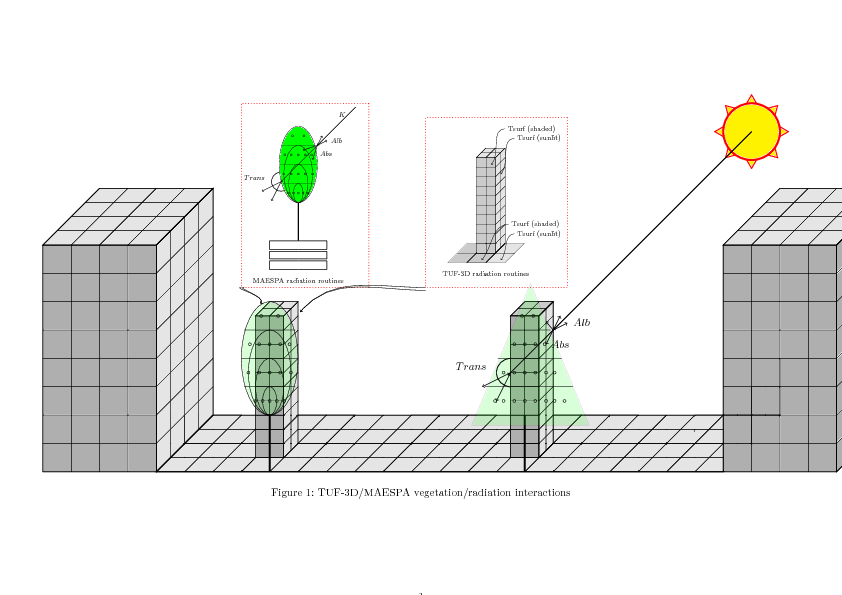
\includegraphics[trim = 35mm 75mm 5mm 81mm, clip, scale=0.28]{images/TUFWithMaespaVegRadiation.png} 
% } 
 \caption{Integration of the tree model MAESPA into VTUF-3D radiation fluxes routines, in which tiled instances of MAESPA vegetation (in green) are used to calculate radiation transmission for VTUF-3D placeholder vegetation structures (in grey)\label{fig:TUFWithMaespaVegRadiation}.}\end{figure}

The second major change required is including the physiological processes of vegetation and soil in the model. Using a novel approach, MAESPA tiles replace VTUF-3D ground surfaces with vegetated MAESPA surfaces and use results of MAESPA's photosynthesis and water balance routines to modify VTUF-3D's energy balance calculations. The vegetation is treated as a flat two dimensional ground surface tile for the surface energy balances. However, each embedded MAESPA surface actually models a full 3 dimensional tree (along with associated soil and vertical movement of water) and feeds results back to VTUF-3D ground surface energy balances (Figure \ref{fig:TUFWithMaespaInsert}). Each grid cell is assumed to hold a single item of vegetation but can theoretically hold multiple items, as supported by MAESPA. In addition, VTUF-3D allows tree canopies to extend into neighbouring grid squares (overhanging the ground, wall, and roof surfaces contained in them and casting shade) so can handle any grid resolution and properly model canopies containing individual trees that exceed the grid size.  

\begin{figure}[!htbp]
 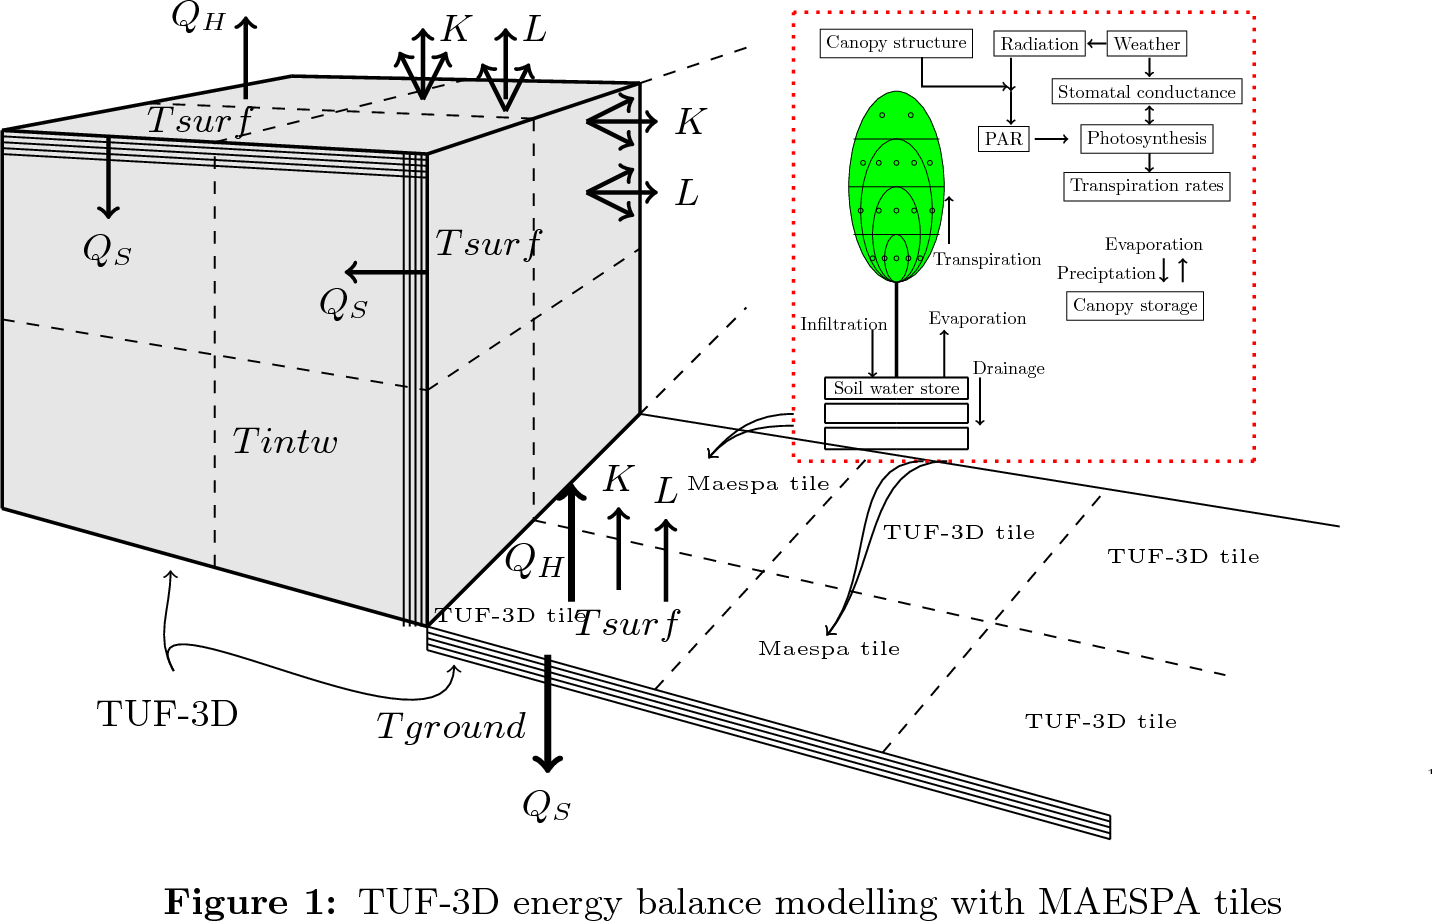
\includegraphics[trim = 0mm 14mm 22mm 0.0mm, clip, scale=0.25]{images/TUFWithMaespaInsert.png}
 \caption{\label{fig:TUFWithMaespaInsert} In VTUF-3D energy balance modelling, ground surfaces can contain either regular TUF-3D surfaces or a surface containing MAESPA modelled vegetation. All surfaces will calculate energy balances at the conclusion of each timestep, partitioning available energy into radiative, sensible, latent, and storage fluxes. Those surfaces with vegetation will also account for vegetation physiological processes when performing energy balances.}
\end{figure}

At the conclusion of each timestep (default of 30 minutes but duration is user configured), VTUF-3D calculates the energy balance of each surface. Tiles of MAESPA instances (with an individual tree or other types of vegetation in each) are used for surfaces that have vegetation (Figure \ref{fig:TUFWithMaespaInsert}). These instances provide values of radiation transmission, energy fluxes (including latent energy, not previously accounted for in TUF-3D), and soil water storage for each item of vegetation in the domain using their unique properties and characteristics. If a surface does not contain vegetation, VTUF-3D runs TUF-3D's normal energy balance calculations.

\subsection{Radiative transfer}\label{sec:radiativetransfer}

In order to track the movement and allocation of radiation, VTUF-3D’s modelling domain is built up in 3D using cubes and their surfaces (facets). To determine which surfaces can `see' each other (unobstructed by other surfaces), ray tracing eliminates pairs of surfaces which will not need to be considered during simulations. Ray tracing also determines sunlit and shaded patterns on the 3D urban surfaces throughout a simulation using a modified version of the \cite{Soux2004} algorithm. Reflections and absorption of longwave and shortwave radiation are modelled using a radiosity approach (radiative reflection and emission treated as perfectly diffuse). These radiative transfer calculations are unchanged from the original TUF-3D scheme and are detailed in \cite{Krayenhoff2007}.

For vegetated parts of the domain, radiative transfer is calculated by components from MAESPA. Incoming radiation, both photosynthetic radiation (PAR) and near infrared (NIR) is partitioned into direct and diffuse using \cite{Weiss1985}. Canopy structure is calculated based on \cite{Wang1990}, supporting a variety of crown shapes namely: conical, half-ellipsoidal, ellipsoidal and paraboloidal. Absorption and scattering of radiation (PAR, NIR, and thermal radiation) by the canopy is calculated using \cite{Norman1979}. Full details of these calculations are included in \cite{Duursma2012}. VTUF-3D accounts for the transmitted and absorbed quantities (as detailed in Section \ref{sec:Representationofvegetation}), however scattered quantities are currently disregarded by VTUF-3D.

In the calculation of net radiation ($Q^{*}_{veg}$) for vegetated grid squares, the TUF-3D calculated $T_{sfc}$ is replaced by MAESPA calculated vegetation surface temperatures ($T_{sfc,veg}$) 

\begin{equation}\label{eq:rnet}
Q^{*}_{veg} = K\downarrow - (\alpha _{veg} K\downarrow) + \epsilon _{veg} L\downarrow - \epsilon _{veg} \sigma  (T_{sfc,veg}) ^{4} 
\end{equation}

where $K\downarrow$ is the downward shortwave radiative flux density (W m$^{-2}$), $L\downarrow$ is the downward longwave radiative flux density (W m$^{-2}$), $\alpha _{veg}$ of vegetation is set to 0.20 and $\epsilon _{veg}$ of vegetation set to 0.97 \citep[p. 12]{Oke1987z}, $\sigma$ is the Stefan-Boltzmann constant (=5.67 $\times$ 10$^{-8}$ W m$^{-2}$ K$^{-4}$), and $T_{sfc,veg}$ is the vegetation surface temperature (K).

\subsection{Convective energy fluxes}

As the simulation proceeds through each timestep, an energy balance is performed on each surface. For each surface with vegetation, the surface temperature ($T_{sfc}$) is set to the value calculated by MAESPA for that tree replacing the TUF-3D calculated value. Using this new value, the following describes modifications to the TUF-3D methods used to partition the energy fluxes of a vegetated surface.

\subsubsection{Latent energy fluxes}
\label{sec:calcleaftemp}
\label{sec:waterbalance}

For latent energy fluxes, $Q_{E,veg}$ is calculated for each grid square, loaded from offline MAESPA modelled data for the individual item of vegetation and accompanying soil in the domain.
These methods are fully described in \cite{Duursma2012} and \cite{Medlyn2007}, but will be highlighted here briefly. MAEPSA uses a number of variations of the Ball-Berry type approach \citep{Ball1987,Duursma2012} for stomatal conductance. Canopy transpiration and leaf temperature for a MAESPA tile is calculated using an iterative scheme based on \cite{Wang1998}. The Penman-Monteith equation \citep{Penman1948,Monteith1965} is applied to each grid point (to account for variations due to sunlit and shaded portions of the canopy) and summed over all the grid points to calculate transpiration. Finally, leaf temperature is found by iteratively closing the energy balance of the leaf, based on \cite{Wang1998}. MAESPA also accounts for water balance functionality. In MAESPA, infiltration is based on a function from the BROOK90 model \citep{Federer2003}. Soil evaporation is based on models developed by \cite{Choudhury1988} and \cite{Williams2001}. Canopy interception of precipitation uses the \cite{Rutter1975} rainfall interception model. Finally, hydraulics of the soil-to-leaf pathway are estimated using the single root model of \cite{Gardner1960}.

VTUF-3D combines MAESPA predicted canopy transpiration and soil evaporation values into a total $Q_{E}$ amount for each vegetated tile. MAESPA outputs values of storage of intercepted rain ($canopystore$), evaporation of wet canopy ($evapstore$), soil evaporation ($soilevap$), and modelled canopy transpiration ($et$) (all in mm) (variables fully documented in \cite{Duursma2016}) that are converted to W m$^{-2}$ for each variable by 

\begin{equation}\label{eq:mmtowm2} 
  Q_{E,et} = et \times A _{mm} \times m_{mol,w} \times \Delta H_{vap} \times c_{w,kj} \times Time  
\end{equation} 
 
where $et$ is evapotranspiration (mm), $A _{mm}$ is the 2-dimensional tree area in mm (mm$^{2}$), $Time$ is the time (seconds), $\Delta H_{vap}$, the enthalpy of evaporation (=42809 J mol$^{-1}$), $c_{w,kj}$, the conversion to watts (=1W/1000KJ/sec), and $m_{mol,w}$, the molar mass of water (=18.0152g mol$^{-1}$). The conversion is performed three more times for the remaining variables.

These values are combined to calculate the total $Q_{E,veg}$ for a grid square in 


\begin{equation}\label{eq:lefromet} 
\begin{aligned}
Q_{E} = Q_{E,et} + Q_{E,soil} + Q_{E,canopy} + Q_{E,evap} 
\end{aligned}
\end{equation}

where each $Q_{E}$ value was previously converted in Equation (\ref{eq:mmtowm2}). With these additions, VTUF-3D is now able to account for $Q_{E}$ in energy balance partitioning, and thus determine the influence of water and vegetation evapotranspiration on temperature predictions in urban canyons.


\subsubsection{Sensible heat and ground storage fluxes}\label{sec:convection} 
Convection in TUF-3D (and thus in VTUF-3D) is implemented as an adaptation of the facet-averaged approach of \cite{Masson2000}. Full details of calculations are described in \cite{Krayenhoff2007}. Horizontal advective exchanges are not considered, which is considered to be a reasonable approach given the well-mixed nature of canopy layer air \citep{Krayenhoff2007}. A more accurate but computationally intensive approach could be undertaken using a computational fluid dynamics (CFD) method. However, forcing by the convection between facets is likely less important than the forcing of surface temperatures through the shaded and unshaded radiation distribution and its interactions of surface material properties \citep{Krayenhoff2007}. There is the possibility that the addition of vegetation to the model will increase the importance of interactions between neighbouring surfaces of varying temperatures and moistures. However, as will be seen in the model evaluation process (Section \ref{sec:Validation}), this simplified approach still delivers suitably accurate results without justifying more computationally intensive methods. 

Using this convective scheme for sensible heat fluxes ($Q_{H}$), vegetation is accounted for differently by modifying the TUF-3D $Q_{H}$ calculations for grid squares with vegetation, using the $T_{sfc,veg}$ of the vegetation instead of the TUF-3D $T_{sfc}$ value in Equation (\ref{eq:qhveg})

\begin{equation}\label{eq:qhveg}
 Q_{H,veg} = h_{i}  (T_{sfc,veg}-T_{can}) 
\end{equation}

where $h_{i}$ is a calculated heat transfer coefficient (W m$^{-2}$ K$^{-1}$) (using \cite{Mascart1995} and the effective wind speed). 


Ground storage flux ($Q_{G}$) calculations of vegetated grid squares are modified from the TUF-3D method for non-vegetated grid squares, and are calculated as a residual of the energy balance equation (where $Q_{G}$ = $Q^{*}$ - $Q_{H}$ - $Q_{E}$). Thus $Q_{G,veg}$ fluxes for grid squares containing vegetation are calculated as

\begin{equation}\label{eq:qgvtuf}
 Q_{G,veg} =  Q^{*}_{veg} - Q_{H,veg} - Q_{E,veg}
\end{equation}


\subsection{Mean radiant temperature and Universal Thermal Climate Index calculations}\label{sec:tmrtutci}

VTUF-3D provides output of incoming and outgoing shortwave and longwave radiation and $T_{sfc}$ for each facet (surface) at each timestep. Air temperature for the canyon, $T_{can}$, is also provided for each timestep. Using these and values of vapour pressure from the forcing data and wind speed at street level, the values for mean radiant temperature ($T_{mrt}$) and the human thermal comfort index UTCI are calculated for each surface. User defined options in the model are available to either calculate $L\downarrow$, using the clear sky formula of \cite{Prata1996}, or use forcing values. Based on this, different options will be used to calculate the following equations.


Calculations of $T_{mrt}$ (\SI{}{\degreeCelsius}) uses a two step procedure. First, globe temperature ($T_{g}$) is calculated by an iterative relaxation solution, using a formulation of \cite{Liljegren2008} in  

\begin{equation}\label{eq:tg2}
\begin{split}
A\epsilon_{g}\sigma T_{g}^{4} &= \frac{A}{2} \epsilon_{g}\sigma( \epsilon_{a} T_{a}^{4} +  \epsilon_{sfc} T_{sfc}^{4} ) \\
&+ \frac{A}{2}( 1-\alpha_{g})(1-f_{dir})S  \\
&+ \frac{A}{4}( 1-\alpha_{g})f_{dir}S /\cos(\theta) \\
&+ \frac{A}{2}( 1-\alpha_{g})\alpha_{sfc}S \\
&- Ah(T_{g}-T_{a})   
\end{split}
\end{equation}

where $A$, is the surface area of a sphere with diameter D of value 0.15m,
$\epsilon_{a}$, the longwave emissivity of the atmosphere, 
$\epsilon_{sfc}$, the longwave emissivity of the surface, 
$\epsilon_{g}$, the globe emissivity (of value 0.95), 
$h$, the convective heat transfer coefficient (W m$^{-2}$ K$^{-1}$) (see Equation (\ref{eq:h})), 
$T_{a}$, the dry bulb air temperature (K) (using $T_{can}$), 
$T_{sfc}$, the surface temperature (K), 
S, the horizontal solar irradiance (W m$^{-2}$) calculated from the total of absorbed and reflected shortwave, 
$\theta$, the solar zenith angle, 
$\alpha_{sfc}$, the surface albedo (of value 0.15),  
$\alpha_{g}$, the globe albedo (of value 0.05), and 
$f_{dir}$, the fraction of the total horizontal solar irradiance, 
$S$, due to the direct beam of the sun. 




The convective heat transfer coefficient, $h$, as used in Equation (\ref{eq:tg2}), is calculated using 

\begin{equation}\label{eq:h}
Nu = 2.0 + 0.6Re^{1/2}Pr^{1/3};  ~~h = k / D Nu
\end{equation}

where $Nu$ is the Nusselt number (-),
$Re$, the Reynolds number (-),
$Pr$, the Prandtl number (-), and 
$k$, the thermal conductivity of the fluid (i.e. air) (W m$^{-1}$K$^{-1}$) \citep{Liljegren2008}.



Depending on user defined scenario model configuration settings, a number of terms in Equation (\ref{eq:tg2}) can use internally calculated values. $\sigma (\epsilon_{a} T_{a}^{4} + \epsilon_{sfc} T_{sfc}^{4} )$ can be replaced with $L\downarrow + L\uparrow$, the result of reflections of $L \downarrow_{i,sky}$. $(1-f_{dir})S$ can be replaced with $K \downarrow_{dif}$, and $f_{dir}S/ \cos(\theta)$ with $K \downarrow_{dir}$. Also, for vegetated grid squares, the terms for $L\downarrow$ and $L\uparrow$ can be replaced with calculations of $L\downarrow$ and $L\uparrow$ from $\epsilon \sigma T^{4}$ where $T_{s,1}$, soil surface temperature (K), is used as the temperature term for the $L\uparrow$ calculation while leaf temperature is used for $L\downarrow$. 

Using $T_{g}$, calculated in Equation (\ref{eq:tg2}), the second step in calculating $T_{mrt}$ proceeds in a formulation of \cite{Kantor2011} 
\begin{equation}\label{eq:tmrtbucket}
  T_{mrt} = 
  \bigg(
   (T_{g}+273.15)^{4} + 
    \frac{1.1 \times 10^{8}  ws_{cm}^{0.6}}{\epsilon_{g}  D^{0.4}}
    \times 
     (T_{g}-T_{a})
    \bigg)^{0.25} - 273.15
\end{equation}
 where $ws_{cm}$ is the wind speed (cm s$^{-1}$).




Finally, the Universal Thermal Climate Index (UTCI) (\SI{}{\degreeCelsius}) for each surface is calculated using the \cite{Brode2009u} UTCI formula, generating UTCI values for each surface, allowing human thermal comfort to be examined in detail across a modelled domain. The calculation uses modelled outputs of air temperature, wind speed (using model calculated wind speed at canyon level), relative humidity (from the forcing data), and $T_{mrt}$ (calculated above). VTUF-3D does not currently calculate a canopy level relative humidity. This is a current limitation and a future enhancement for the model. But as will be shown in the evaluation of VTUF-3D focussing on urban canopy layer air temperature, $T_{mrt}$, and UTCI predictions (Section \ref{sec:CoMValidations}) and in the energy flux evaluation (Section \ref{sec:PrestonValidation}), the model still performs well despite this limitation. 

%This UTCI formula was designed to provide human thermal comfort assessments using thermal environment parameters with fixed values (incorporated into the formula) for metabolic rates and clothing levels \citep{Brode2012a}. While future development is needed to provide wider flexibility to vary metabolic rates and clothing levels, existing versions of this formula were developed to embody equivalent human physiological responses to differing thermal parameters \citep{Havenith2012,Fiala2012}.

\subsection{New VTUF-3D shading logic integrating vegetation shading}\label{sec:integration}
In order to understand the changes made to create VTUF-3D, an overview of the TUF-3D logic is necessary. Two dimensional (x,y) locations of building locations are configured along with their heights. TUF-3D uses forcing data of temperature, humidity, incoming radiation levels, and wind speed and direction from a location at specified z height (above the canopy). Wind is used in roughness calculations but not used to resolve movements around the buildings (as a CFD based model would). This simplification is a design decision trade-off to reduce the complexity of the model and the intensity of computations, while still producing robust enough results.



\begin{figure}[!htbp]
   \subfloat[Initial view angles ray tracing.]{
   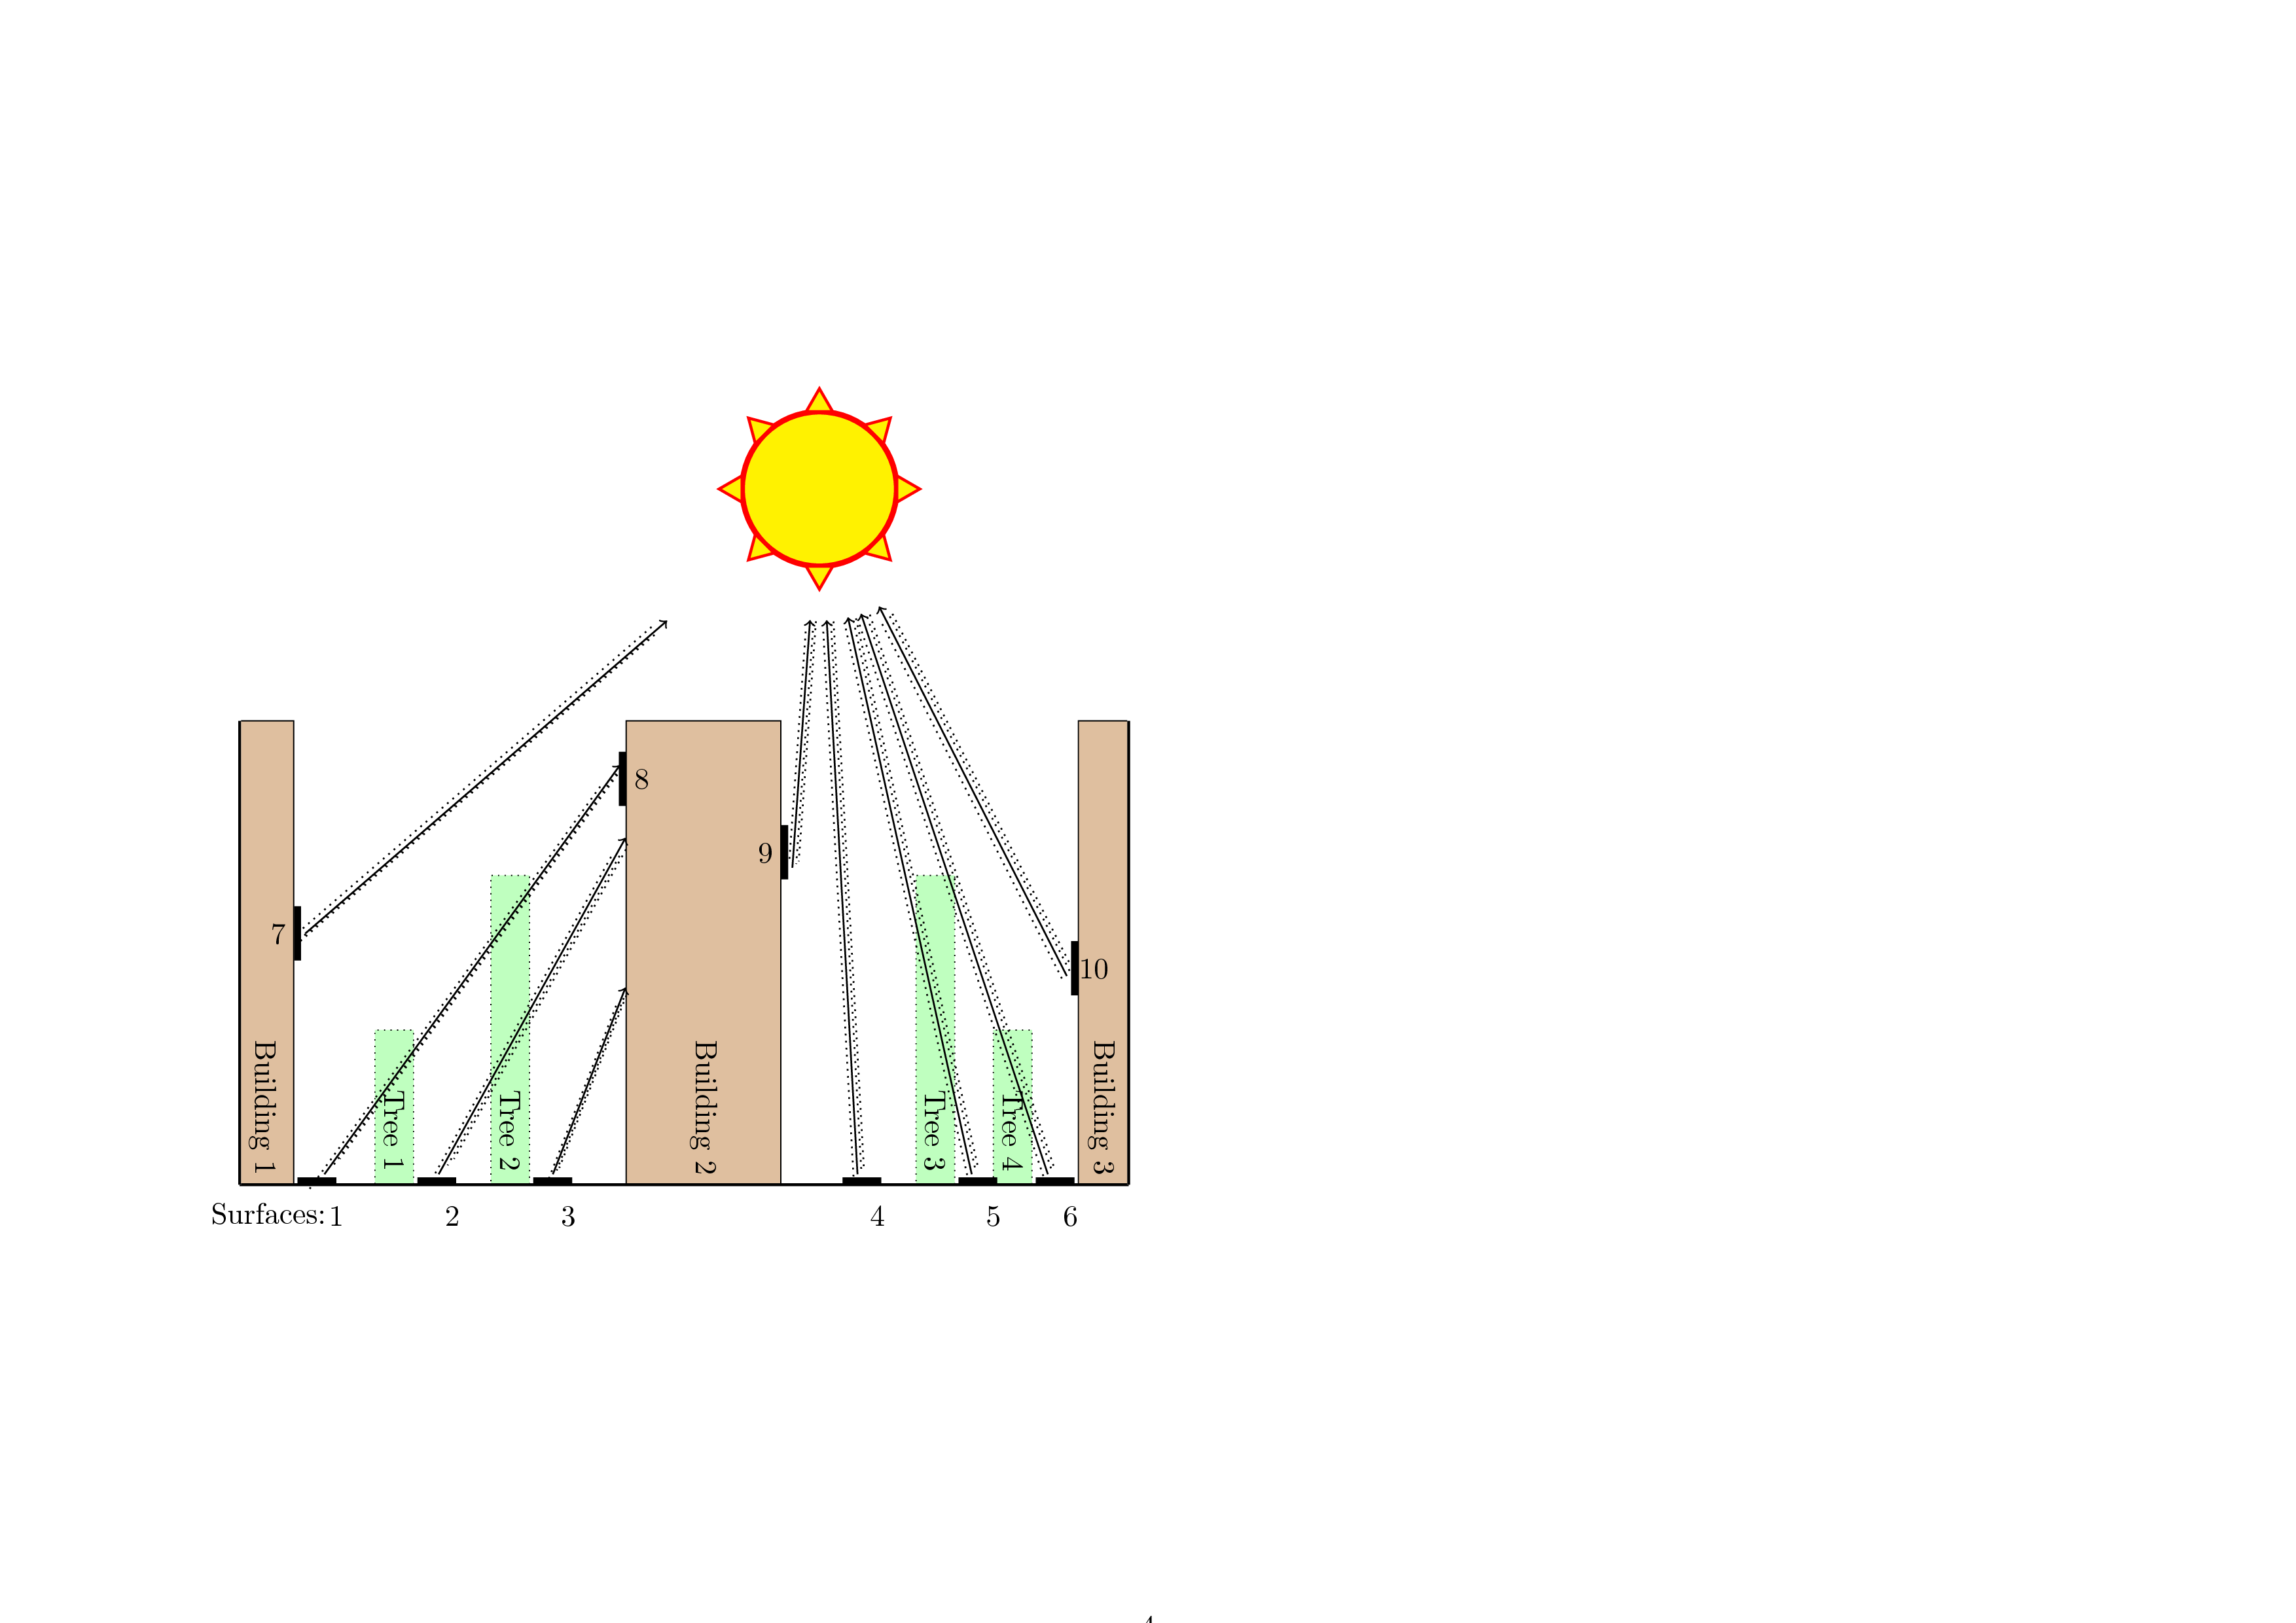
\includegraphics[trim=110mm 211mm 621mm 210mm, clip, scale=0.15]{images/VTUF-Design-3.png}
   }
  \hspace{0.5cm}  
   \subfloat[TUF-3D unmodified shading.]{
   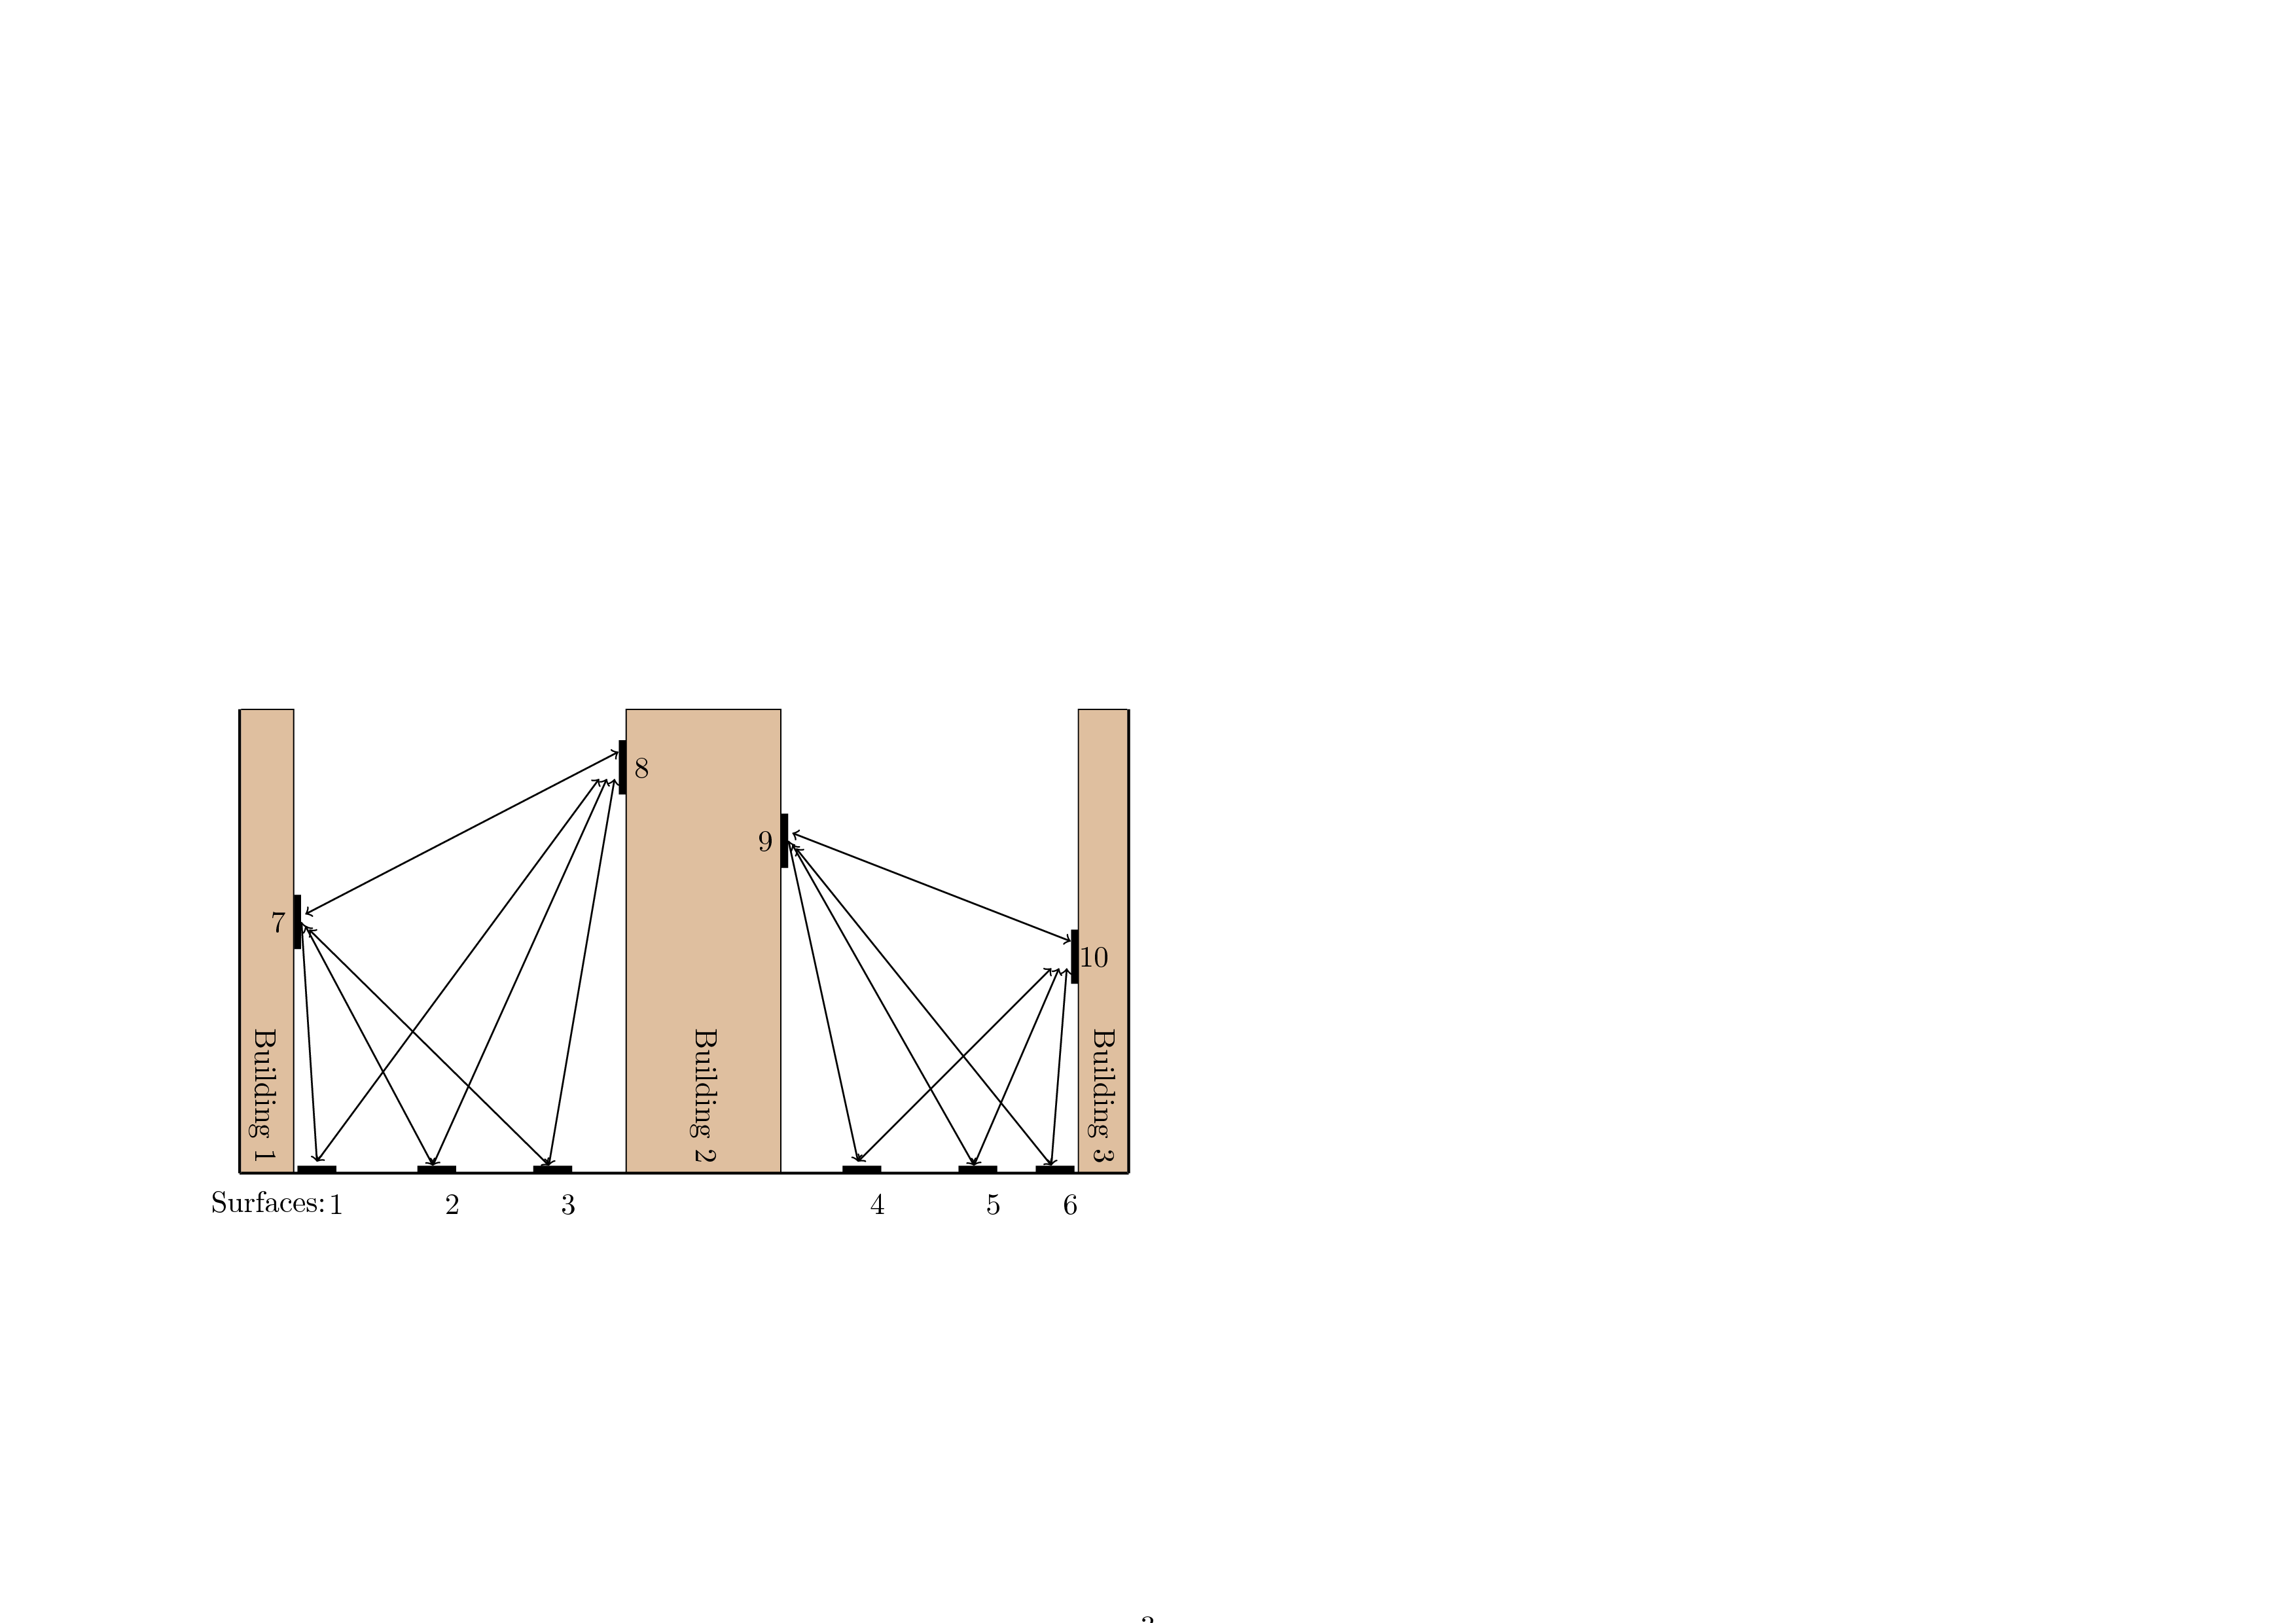
\includegraphics[trim=110mm 211mm 621mm 210mm, clip, scale=0.15]{images/VTUF-Design-2.png}
   }
  \hspace{0.5cm}
  \\
   \subfloat[VTUF-3D modified shading.]{
   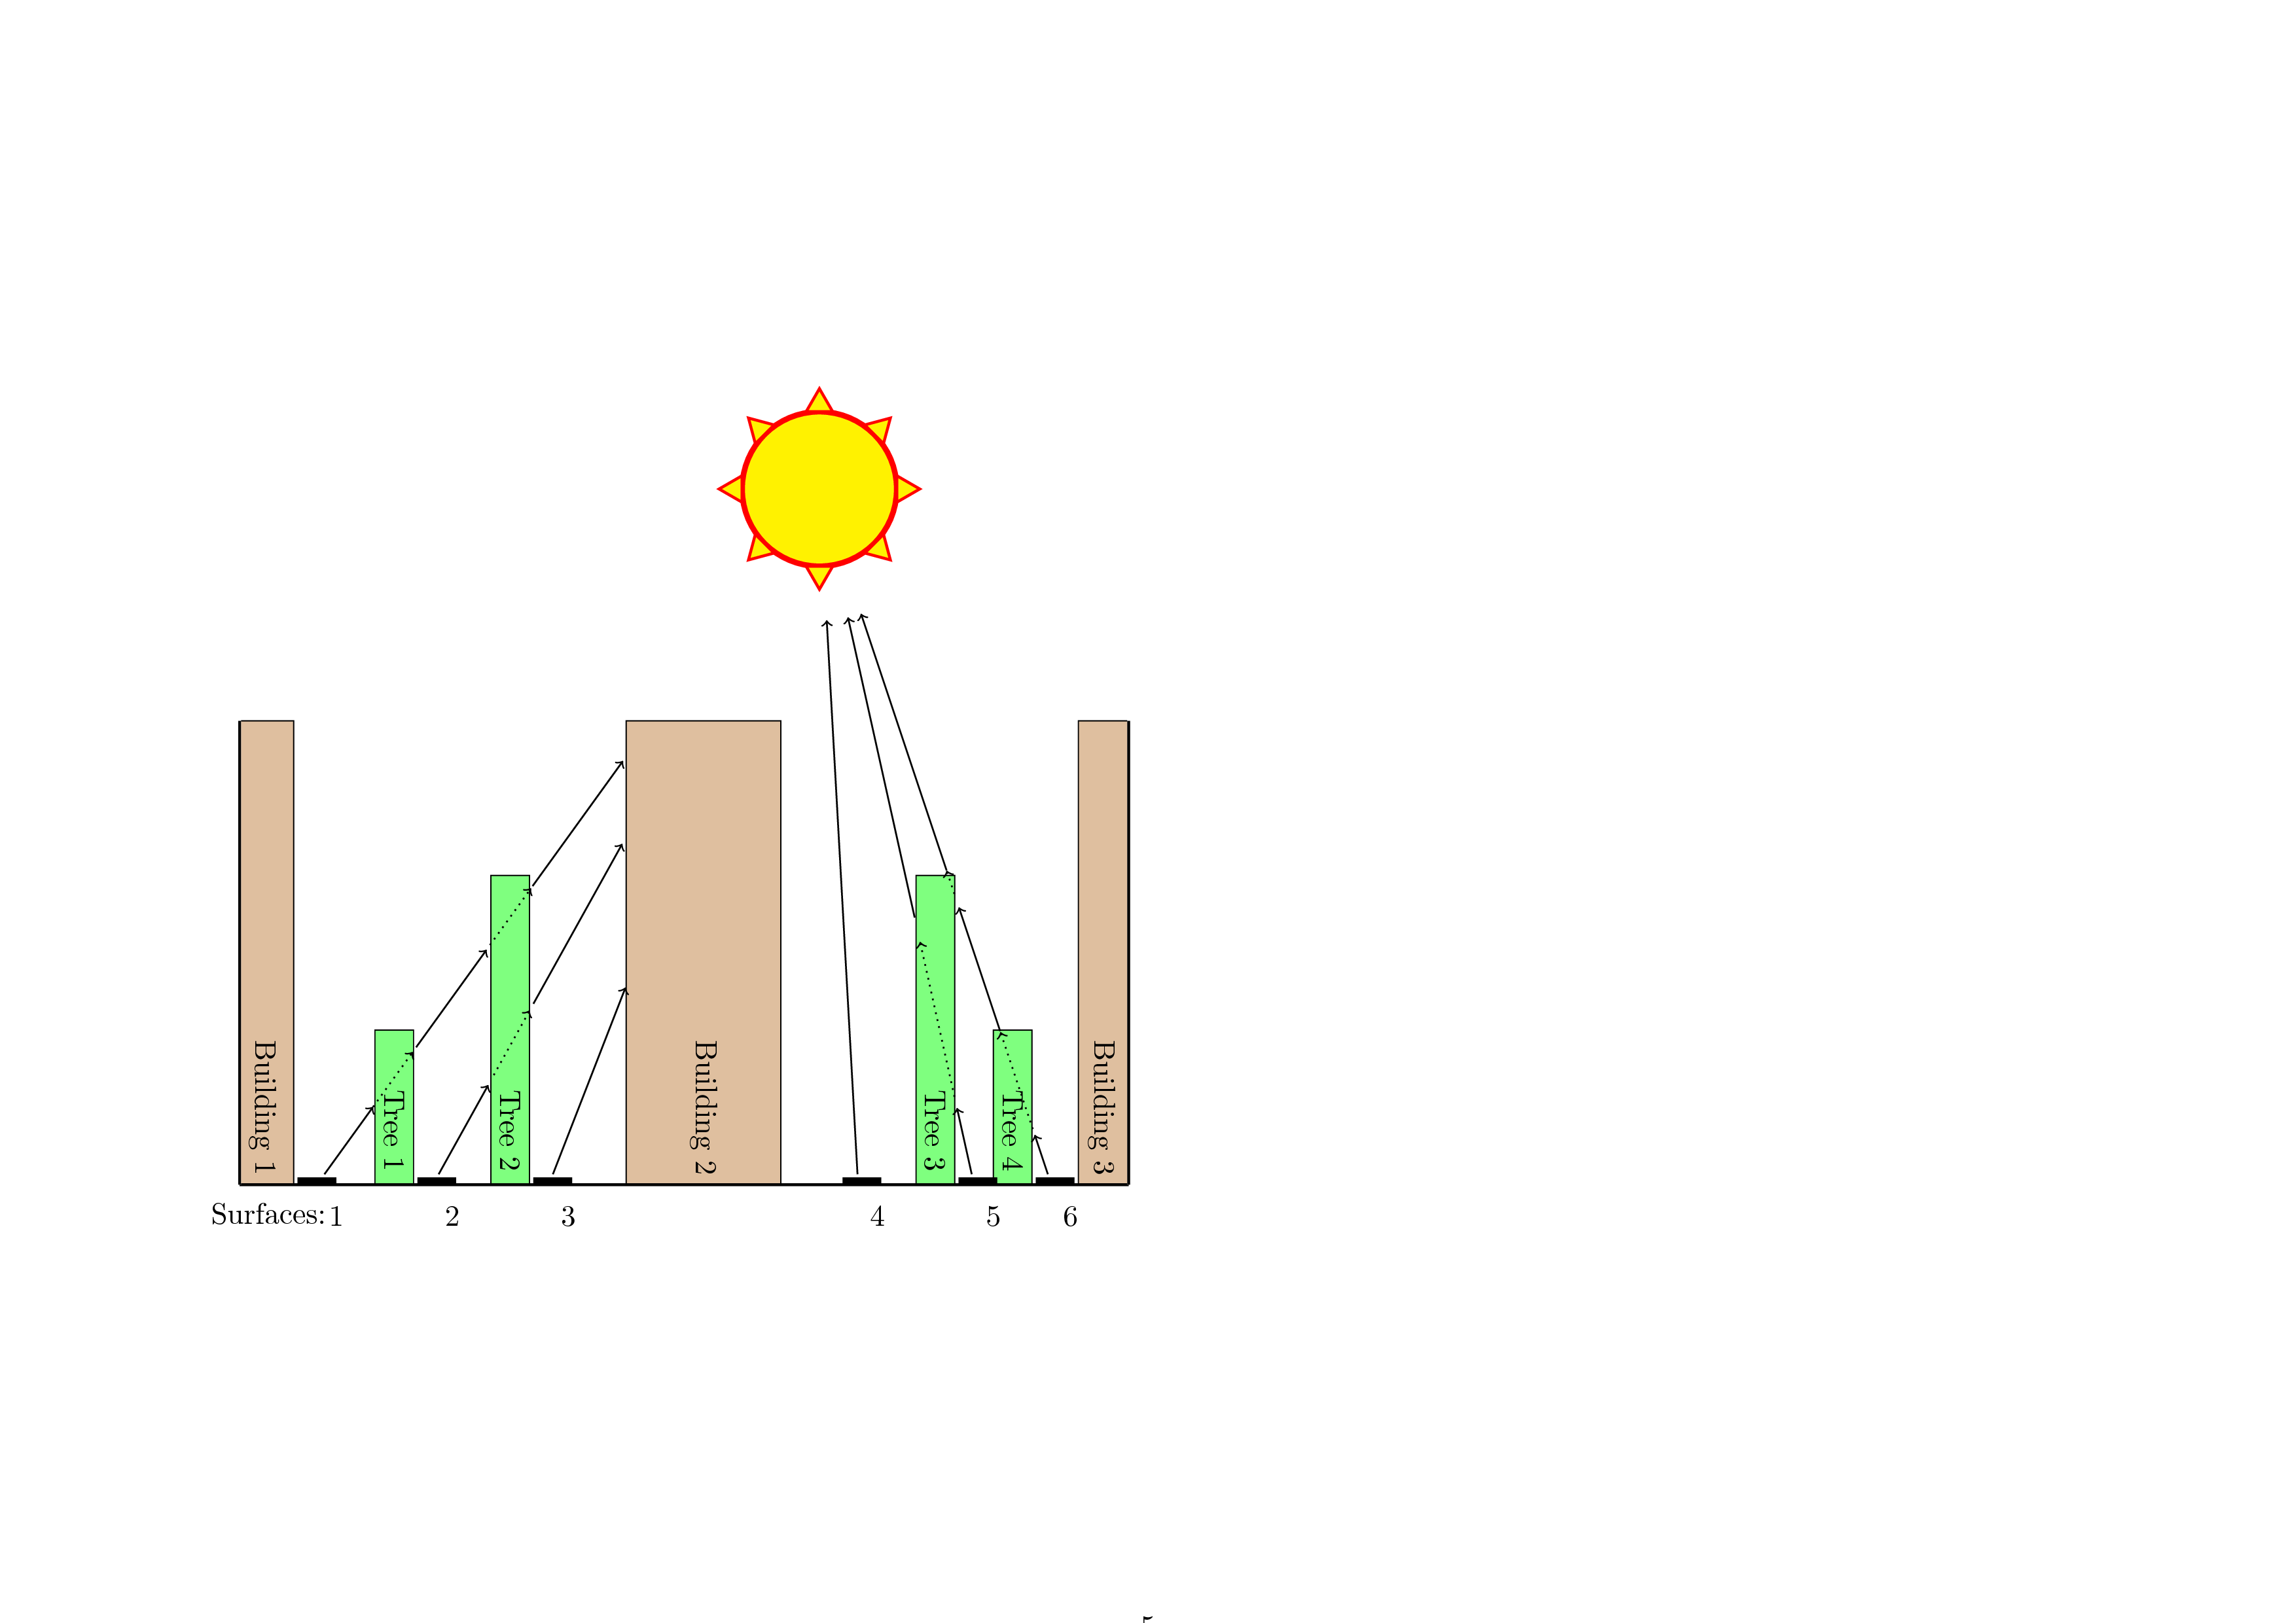
\includegraphics[trim=110mm 211mm 621mm 210mm, clip, scale=0.15]{images/VTUF-Design-4.png}
   }
  \hspace{0.5cm}
   \subfloat[VTUF-3D reverse ray tracing.]{
   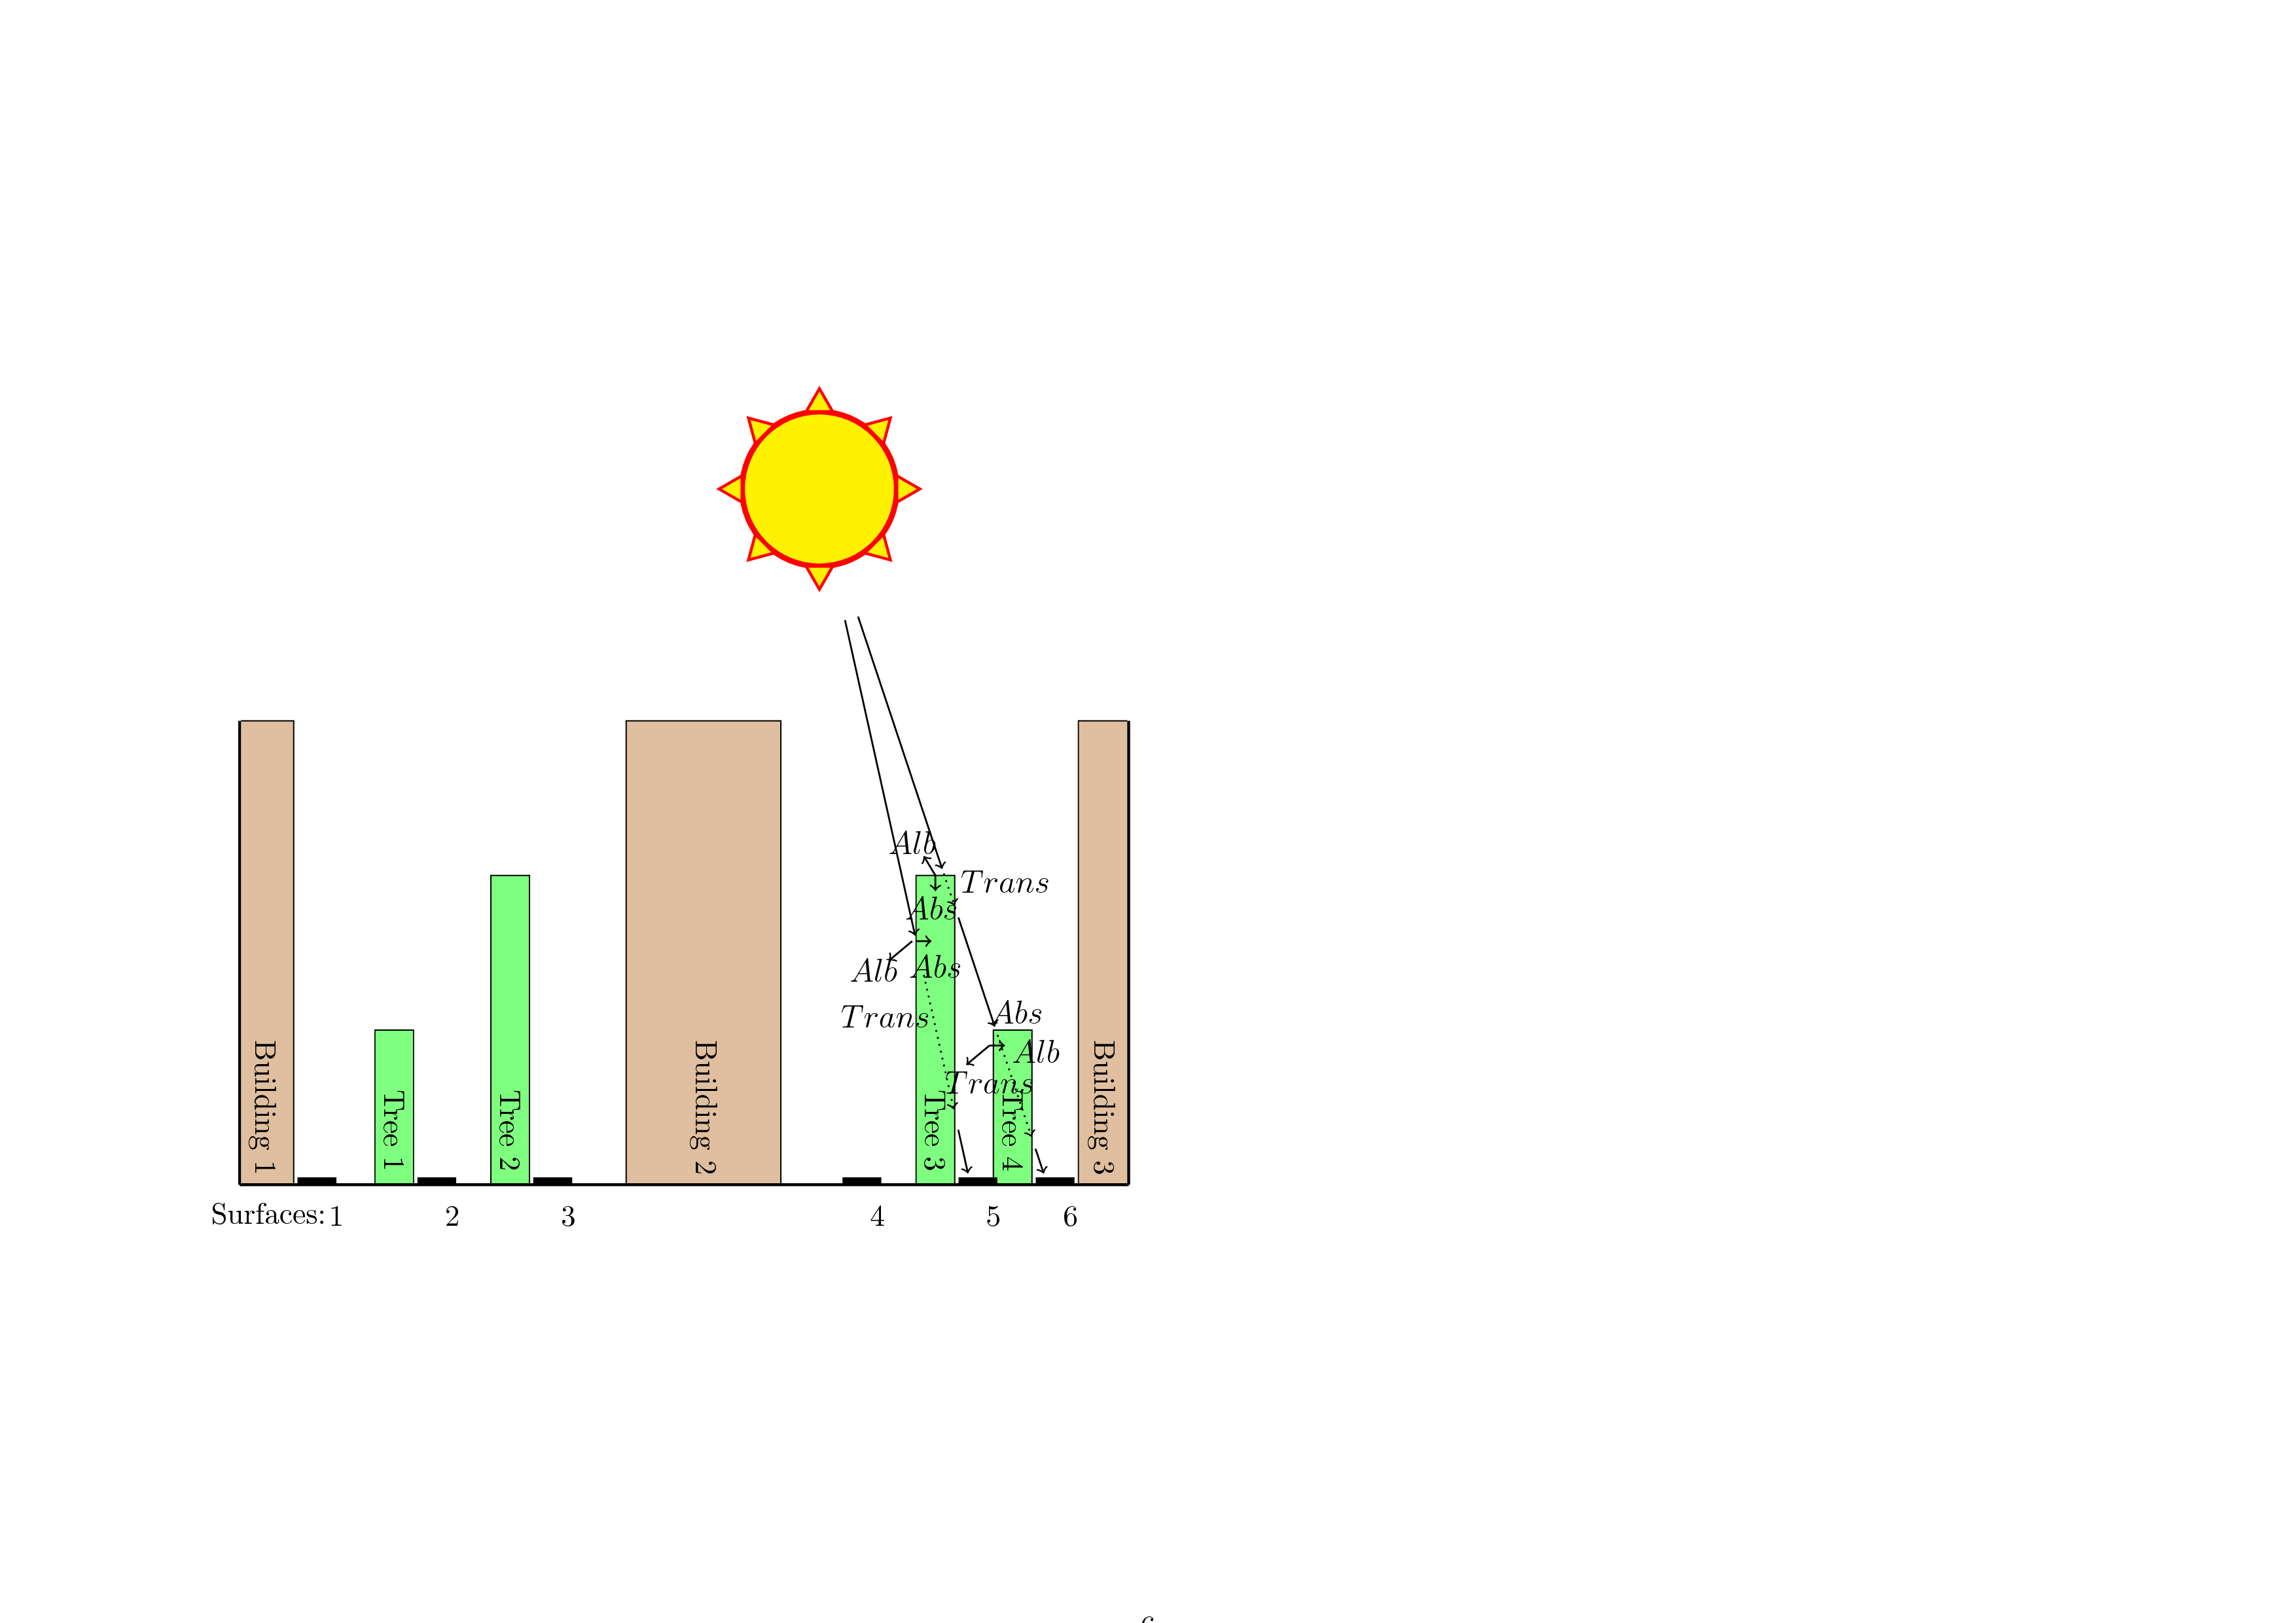
\includegraphics[trim=110mm 211mm 621mm 210mm, clip, scale=0.15]{images/VTUF-Design-5.png}
   }
   \caption{(a) Initial view angles ray tracing, run during model initialisation to determine which surfaces are visible to each other. Trees depicted with dashed borders to emphasise they are present in the domain but are not considered at this point in the simulation. \label{fig:initray} (b) TUF-3D unmodified shading logic in which each surface performs four ray traces (from each surface quarter) towards the sun and determines sunlit percentage based on how many rays leave the domain without meeting an obstruction. Vegetation modelling is not possible in TUF-3D, so is not depicted. \label{fig:shading} (c) VTUF-3D modified shading, timestep ray tracing, using the same process as the unmodified logic but setting a flag for any ray that encounters vegetation. \label{fig:modshading} (d) VTUF-3D modified shading, reverse ray tracing. For any rays that encounter vegetation in forward ray tracing, reverse ray traces are performed to allocate radiation to intervening encountered surfaces. \label{fig:modshadingreverse}} 
\end{figure}


The domain initialisation ray tracing routines of TUF-3D have not been modified. In these (Figure \ref{fig:initray}a), unnecessary interactions are determined during the model initialisation process by finding which surfaces are visible to each other and which pairs of surfaces are fully obstructed by other surfaces and need not be considered in determining radiation exchanges. Then, as the model runs the main simulation, at each timestep, TUF-3D runs a shading routine (Figure \ref{fig:shading}b). In it, the model iterates through each surface in the domain (roads and building walls and roofs), tracing rays four times from each quarter of the surface towards the sun to determine that surface's level of illumination, yielding results of 0, 25, 50, 75, and 100\% illuminated. By using these sunlit levels, each surface can be allocated the appropriate amount of incoming radiation during the energy balance process.



\subsubsection{Integrating vegetation shading and modified ray tracing logic in VTUF-3D}\label{sec:Representationofvegetation}

After model improvements to VTUF-3D were made, a similar parallel logic was created to represent the vegetation in the domain. These vegetation elements are ignored in the initial ray-tracing (Figure \ref{fig:initray}a). This initial ray tracing is performed to optimise the modelling, to exclude any two surfaces which will never be visible to each other. However, depending on the density of the vegetation, the pathway between two surfaces might not be completely obscured by vegetation so these cases will have to be evaluated during the simulation run.

At each timestep during the simulation, VTUF-3D now runs a modified shading routine (Figure \ref{fig:modshading}c). During the model iteration through each surface in the domain, ray-traces towards the sun are done as described previously (the TUF-3D default method). However, each step of the ray trace checks to see if vegetation has been encountered, and if encountered, sets a flag to indicate further processing will be needed. Then the ray trace continues and concludes when it either passes out of the domain or is blocked by a building. If no vegetation is encountered, radiation exchanges between surfaces along the ray default to the original TUF-3D method. Otherwise additional processing needs to be done to account for the radiation exchanges affected by vegetation.

To resolve the sunlit factor for surfaces that encountered vegetation during the ray trace, reverse ray tracing is done for those beams (Figure \ref{fig:modshadingreverse}d). For surfaces 5 and 6 in Figure \ref{fig:modshadingreverse}d, ray tracing is done from the top of the domain back along the radiation path. When the ray encounters vegetation (surfaces 5 and 6), VTUF-3D looks up the tree associated with the ground surface below and loads the offline calculations of the amount of radiation reflected, absorbed, and transmitted through the vegetation. The ray tracing continues, allocating the remaining radiation either to further intercepting vegetation or ultimately to the final ground or building surface.

Each item of vegetation in the domain is modelled offline and this data is made available for the main simulation run. In order to account for the effects of inter-tree shading or shading by buildings during the main simulation run, these offline vegetation calculations are run twice using varied amounts of incoming shortwave. The first variation uses 100\% incoming solar radiation to account for when the vegetation is in full sun. The second variation uses only the diffuse component of the incoming solar radiation for when the vegetation is shaded by obstructions. The proper variation for each item of vegetation is chosen programmatically (based on its current sunlit percentage) during the model run. As the illumination levels vary in each location in an urban canyon across the diurnal cycle, these variations allow the differing vegetation responses (varying levels of photosynthesis due to lower levels of PAR, changes in surface temperatures, and varying vegetation evapotranspiration due to differences in stomatal conductance and vapour pressure deficits) to be captured. However, these variations will not be able to exactly capture every variation, such as a reduction in diffuse shortwave due to a nearby building. Examples of the forcing data required for these offline variations are described in the Pr04Val evaluation set-up (Section \ref{sec:modelsetup}).

\section{Model evaluation}\label{sec:Validation}
\subsection{Energy flux predictions evaluation}\label{sec:PrestonValidation}
Evaluations of VTUF-3D need to be performed to ensure that this new model is making accurate predictions. As an energy balance model, modelled output comparisons to observations of energy fluxes and temperatures are considered fundamental evaluations \citep{Masson2002a}. With the addition of vegetation modelling, it is important that those aspects are also properly evaluated. 

\subsubsection{Evaluation data}

An evaluation was performed based on flux tower observations recorded in the suburb of Preston, in northern Melbourne, Australia \citep{Coutts2007}. Preston is a homogeneous, low to medium density area and characterised as LCZ6B (open low-rise) \citep{Stewart2012b}. A 40 meter flux tower recorded observations during 2003 and 2004 \citep{Coutts2007}, providing observed values of $Q^{*}$, $Q_{H}$, $Q_{E}$, air temperature, humidity, wind speed and direction. $Q_{G}$ was calculated as a residual of the surface energy balance. Estimates of the anthropogenic heat flux ($Q_{F}$) were made using an inventory approach, though $Q_{F}$ is included implicitly in the observations and contributes to the observed sensible heat fluxes. The use of this data set allows an evaluation of surface energy balances against modelled predictions. This data set was also used as the forcing and comparison data set for Phase 2 and 4 of the International Urban Energy Balance Models Comparison Project \citep{Grimmond2011,Best2012}. Phase 2 of this comparison project evaluated the performance of 32 urban land surface modelling schemes, forced by and compared to these observations, using a consistent methodology. Phase 4 re-evaluated many of these modelling schemes for their performance across a variety of seasonal cycles.

\subsubsection{Evaluation set up}\label{sec:modelsetup}

The modelled domain (100x100m with a 5m grid resolution) was an area of interest (AOI), chosen to be representative of the overall land cover influencing the fluxes at the tower (Figure \ref{fig:PrestonModArea}). Aerial imagery from 2015 \citep{GooglePreston2015} was used as an initial basis for the modelling domain. The measurement height for the observations ensured that the measured fluxes well represented the local scale (approximately 1000 meters) of the area \citep{Coutts2007}. Additionally, the site selection ensured a homogeneous nature of the overall flux coverage area \citep{Schmid1994}. Because of this, the micro-scale modelled domain is representative of the fluxes observed at a local scale. This is confirmed by the land surface classification of the site. \cite{Coutts2007} undertook a land surface classifications to support interpretation of the 2003-04 flux data, from aerial imagery (from 2002) within a 500 m radius of the observation tower. The selected AOI (Figure \ref{fig:PrestonModArea}) is in good agreement with the 500 m radius classification of \cite{Coutts2007} with respect to the pervious/impervious fractions. Breakdowns of both classifications, and the 100m x 100m domain used here are shown in Table \ref{tab:expertValues}. Overall, the modelled domain selection is very similar to the broader area, is representative of the local scale and will allow an appropriate comparison between the observed and modelled results. In addition to the land cover fractions, other properties of the observation site are listed in Table \ref{tab:prvalpara}.

\begin{figure}[!htbp]
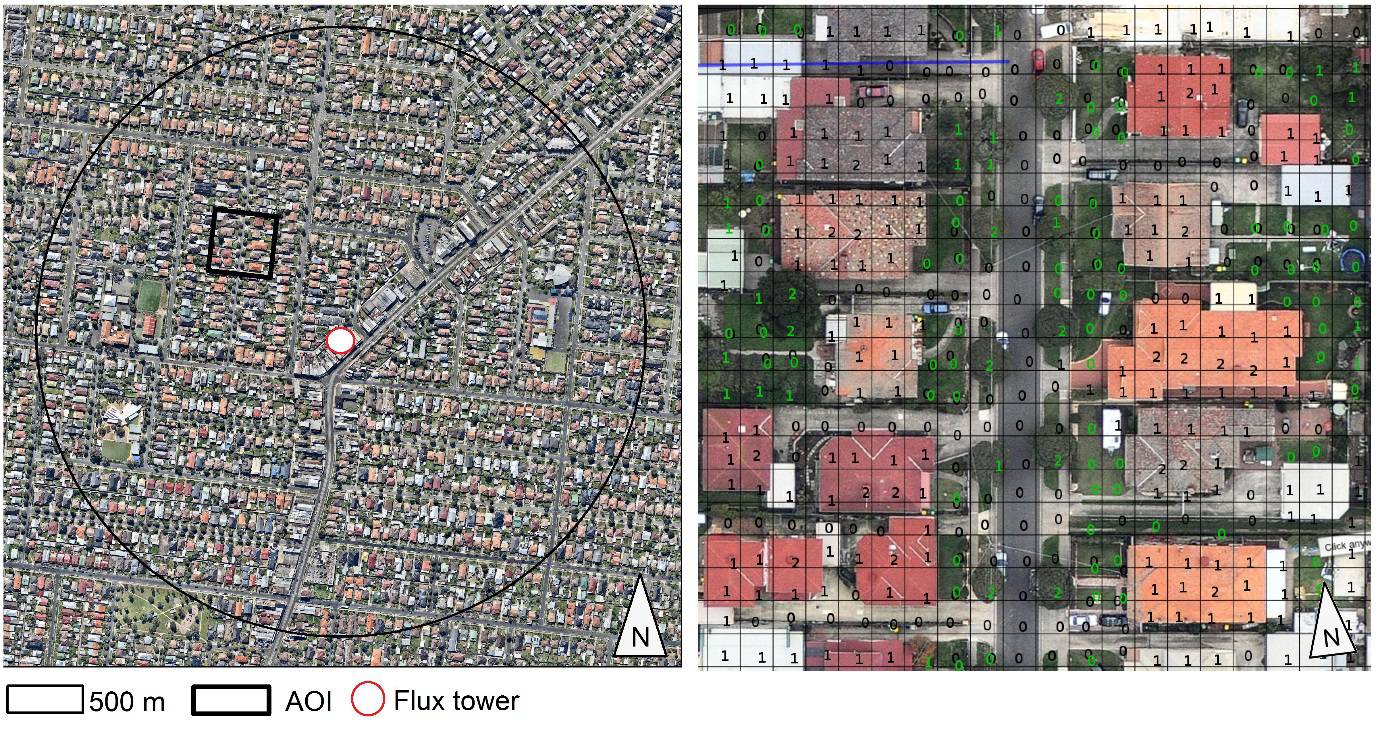
\includegraphics[trim = 0mm 0mm 0mm 0mm, clip, scale=1.00]{images/PrestonModelledArea.png} 
\caption{Observed Preston suburb showing 500m effective radius of flux tower observations. Black box annotates model domain area of interest (AOI). Adapted from \cite{GooglePreston2015}.\label{fig:PrestonModArea} / Digitisation of AOI, Preston suburban street, Oakhill Ave. Building heights in black, vegetation heights in green (in 5m units). Adapted from \cite{Nearmap2015}.\label{fig:PrestonDigitization}}      
\end{figure}



\begin{table}[!htbp]
\caption
{Preston land cover classification of a 500m radius from the observation tower from \cite{Coutts2007} and \cite{Nury2015}, and the classification of the model domain area of interest (AOI) (all in percentages). \label{tab:expertValues}} 
\begin{tabular}{ |c |c| c | c |c |c |c|p{1.65cm}|p{1.65cm}| } 
\hline \textbf{Source} & \textbf{Blg.}&	\textbf{Imp.}&\textbf{Tree}&\textbf{Grass}	&\textbf{Water}&\textbf{Tot. Imp.}&\textbf{Tot. Per.} \\ \hline
\textbf{500m radius} & & & & & &	&  \\ \hline 
\cite{Coutts2007} &44.5 &17.5&22.5 &15.0 &0.5 &62.0 &38.0	  \\ \hline 
\cite{Nury2015} &32.0 &34.5 &10.1 &23.4 &0 &66.5 &33.5  \\ \hline 
 & & & & & &	&  \\ \hline 
AOI (100x100m) &45.2 &19.3 &16.0 &19.5 &0 &64.5	&35.5  \\ \hline 
\end{tabular} 
\end{table}  
 
\begin{table}[!htbp]
\caption{Preston evaluation site properties \citep{Coutts2007}. \label{tab:prvalpara}}     
\begin{tabular}{| l | l |}
\hline
\textbf{Property} & \textbf{Value(s)} \\ \hline
$\alpha$, albedo & 0.15  \\ \hline
$z_{m}$, instrument height (m)&  40  \\ \hline
$z_{0}$, roughness length (m)& 0.4  \\ \hline
$z_{h}$, maximum height of roughness elements (m)& 12  \\ \hline
$z_{b}$, mean building height (m)& 6.4  \\ \hline
$H:W$, mean height to width ratio& 0.42  \\ \hline
$W:P$, mean wall-to-plan ratio &0.4  \\ \hline
\end{tabular}
\end{table}

The 2015 imagery used here for the model domain was 13 years after the 2002 imagery used in \cite{Coutts2007}. In a remote sensing study by \cite{Nury2015} examining urban greenery and heat mitigation, a land cover classification of the Darebin Council area (55.6 km$^{2}$) (which includes Preston) was performed using aerial imagery from 2009 and LIDAR data from 2008. This land surface classification was much improved in terms of accuracy (due to higher quality and higher resolution imagery) than that of \cite{Coutts2007} and provided a more recent set of land surface data (Table \ref{tab:expertValues}). Some differences in the classification were seen, with the \cite{Nury2015} classification showing a lower building fraction and a higher impervious surfaces. Further, some reduction in vegetation cover is seen between the \cite{Coutts2007} classification and the \cite{Nury2015} classification. This introduces a small amount of uncertainty in the exact make-up of the modelling domain and could explain some of the low predictions of Q$_{E}$ seen later in this evaluation. While the \cite{Nury2015} dataset was generated from different resolution imagery and from a later time period, it does show very good agreement with the total impervious/pervious fraction of the 500m classification.


Model parameters were set to the values given in Table \ref{tab:modprvalpara} and domain parameter values in Table \ref{tab:expertValues}. Most of these values are TUF-3D default values, from \cite{Krayenhoff2007}. The modelled domain is a digitisation of the AOI, Oakhill Ave. in Preston (Figure \ref{fig:PrestonModArea}) with building locations and heights as shown in Figure \ref{fig:PrestonBldHt}.


\begin{table}[!htbp]
\caption{Preston evaluation scenario model parameters. \label{tab:modprvalpara}}     
\begin{tabular}{| p{8.0cm} | l | l|}
\hline
\textbf{Parameter} & \textbf{Value(s)} & \textbf{Source}\\ \hline
Albedo (roof, street, wall)   & 0.15, 0.10, 0.30   & \cite{Krayenhoff2007}\\ \hline
Emissivity (roof, street, wall)   & 0.92, 0.92, 0.88   & \cite{Krayenhoff2007}\\ \hline
Forcing data height (m)  & 40   & \cite{Coutts2007} \\ \hline
Mean height of buildings (m)  & 5.61   & Calculated from domain \\ \hline
Mean height of trees (m)  & 5.7   & Calculated from domain \\ \hline
Initial $T_{sfc}$ (roof, street, wall) (\SI{}{\degreeCelsius})  & 18.0, 23.0, 22.0  & \cite{Krayenhoff2007}  \\ \hline
Constant building internal air temperature (base of roofs and walls) (\SI{}{\degreeCelsius})  & 22.0, 20.0 & \cite{Krayenhoff2007}   \\ \hline
Constant deep-ground temperature (\SI{}{\degreeCelsius})  & 19.0  & \cite{Krayenhoff2007} \\ \hline
Constant building internal floor temperature (\SI{}{\degreeCelsius})  & 15.0  & \cite{Krayenhoff2007} \\ \hline
\end{tabular}
\end{table}

\begin{figure}[!htbp]
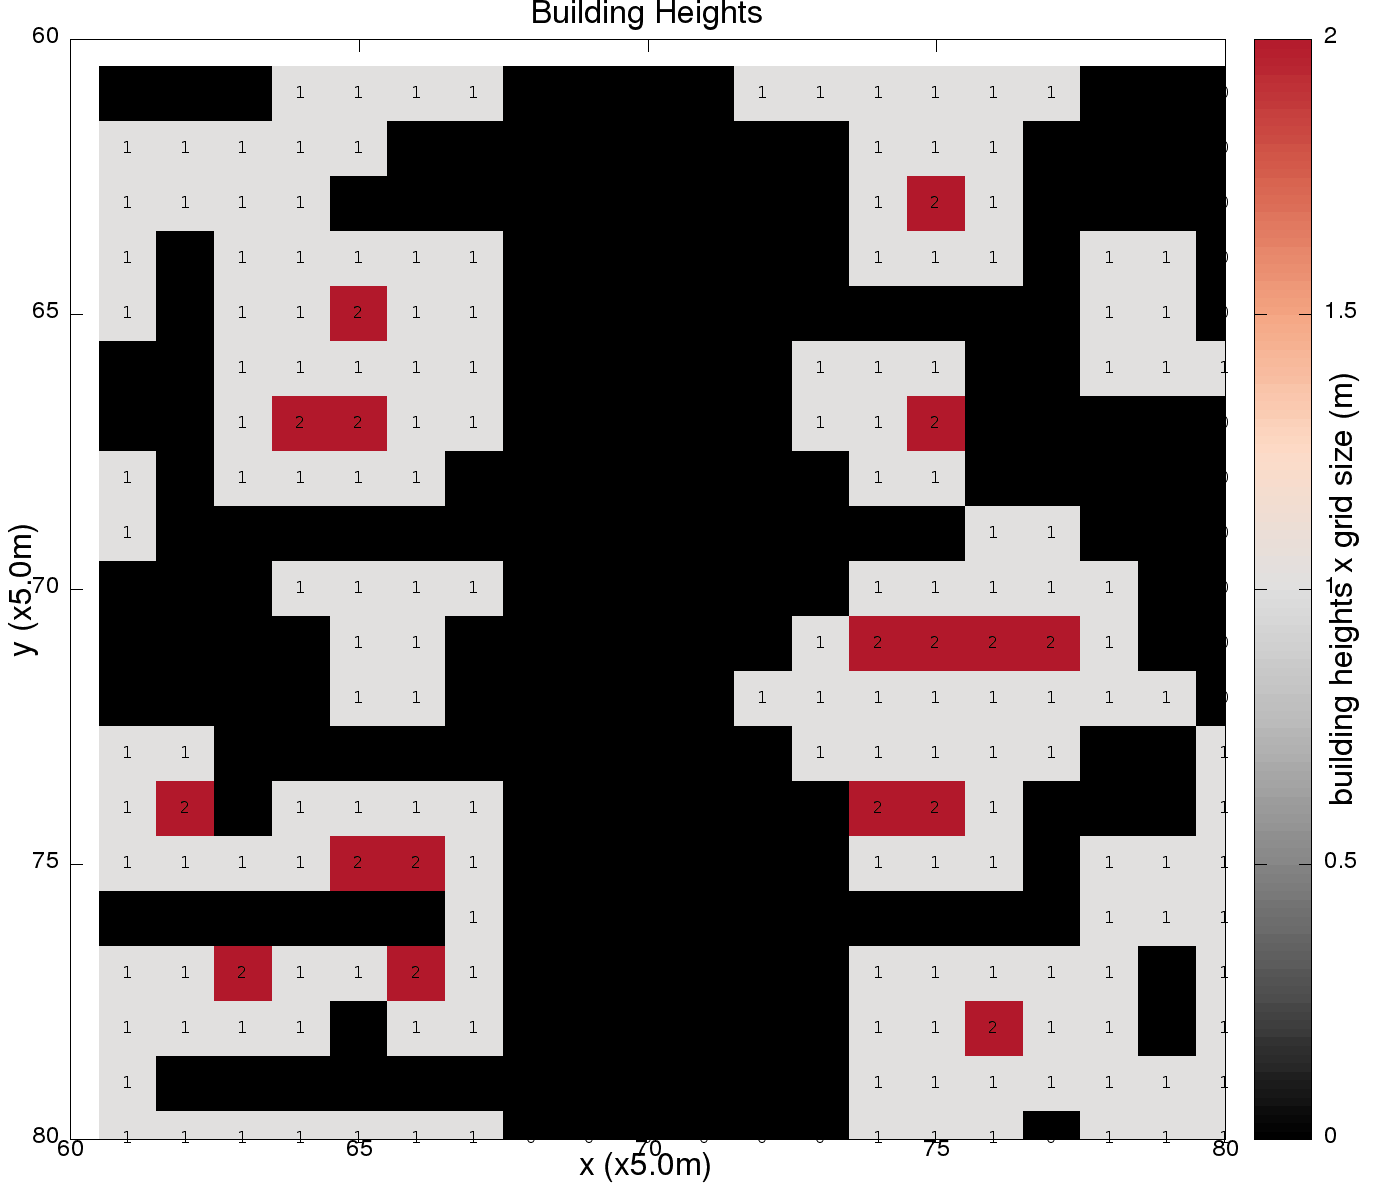
\includegraphics[trim = 0mm 0mm 0mm 0mm, clip, scale=0.20]{images/CentralBuildingHeights.png} 
\caption{Preston evaluation domain configured building heights (0, 5, 10m) and locations for modelling scenario Pr04Val.\label{fig:PrestonBldHt}}      
\end{figure}

Vegetation (trees, shrubs, and ground cover) is added to VTUF-3D by populating physiological and physical parameter values (using observed or literature values) in configuration files. This means any species or type of vegetation can be included in VTUF-3D. Two tree types were employed in this evaluation, namely \textit{Olea europaea} (Olive) and \textit{Lophostemon Confertus} (Queensland brushbox), as well as turf grass, \textit{Festuca arundinacea} (Tall Fescue). The detailed parameterisations for these vegetation types are shown in \ref{sec:maespavegpara}. A mix of 25\%/75\% \textit{Olea europaea} and \textit{Lophostemon Confertus}) trees were used in the model. Identifying and parametrising every tree species in the domain can be time consuming, so our parametrisations were limited here to these species. The species mix was chosen to best account for density of canopy cover in the aerial imagery but given this limitation, will not completely reflect the observed species mix and might create some modelling errors from the observed fluxes. However, the two available species are representative of commonly planted trees in Melbourne. A street tree inventory by \cite{Frank2006} finds that \textit{Lophostemon Confertus}, a native evergreen, is the most common street tree, representing 6.9\% of street trees in Melbourne. Olive trees are considered suitable for Melbourne's climate conditions (drought tolerant evergreen) and a recommended species for council street tree planting \citep{PortPhillip2010}.

The evaluation simulation (which is named Pr04Val) was run for 30 days, from 10 February 2004 to 10 March 2004, forced by the observations from \cite{Coutts2007} for those days. Meteorological forcing included $K\downarrow$, $L\downarrow$, air temperature, wind speed, wind direction, and air pressure at a height of 40m. Forcing data for the vegetation components use shortwave values of mean global and mean diffuse observations taken from one minute solar observations (station 086282, Melbourne Airport) \citep{BOM2016}. For full radiation vegetation runs, the mean global irradiance was used while for diffuse runs, the mean diffuse irradiance was used. In addition, the MAESPA FBEAM variable (fraction of incident PAR which is direct-beam) is set to 0.0 in the forcing data for diffuse runs.

The evaluation period contained a range of conditions. The period especially features a number of hot days (over \SI{30}{\degreeCelsius}). As one of the major applications of VTUF-3D will examining the potential for moderating urban heat through urban vegetation, evaluation over a period containing hot days is important. The observation period also contains a number of days with precipitation. In the current VTUF-3D design, precipitation will only be received in grid squares that contain vegetation and pervious surfaces. The expected impact of this is that predictions of $Q_{E}$ will be understated for days that contain precipitation. Accounting for rainfall on impervious surfaces is a current limitation of VTUF-3D (to be addressed in later versions of VTUF-3D) and caution should be used in modelling periods which contain significant rainfall. For the intended primary use of VTUF-3D, examining temperature moderation during the hottest periods of the year (often containing little rainfall), rainfall limitations should be less of an issue. Also, in most urban areas, precipitation on impervious surfaces will be rapidly removed as stormwater.

\subsubsection{Evaluation approach}\label{sec:prvalresults}

The evaluation scenario (named Pr04Val) compares the modelled results for the 30 day run with the observed fluxes ($Q^{*}$, $Q_{H}$, $Q_{G}$, and $Q_{E}$) for the domain that aligns well with the land surface classification for the wider local scale area (Table \ref{tab:expertValues}). Comparisons with the observations were performed using the \cite{Willmott1981} d index of agreement. In addition, the VTUF-3D model was run with a `no vegetation scenario', undertaken to demonstrate the significant improvement of the model. This scenario (named Pr04NoVeg), represents an unimproved TUF-3D without vegetation modelling capability, as the lack of vegetation will not trigger any of the new logic and improvements added to the model. Finally, as the observations used in this evaluation are the same as in Phase 4 of the Intercomparison project \citep{Best2012}, using the \cite{Coutts2007} Preston dataset, the performance of the VTUF-3D model can also be placed within the intercomparison evaluation of urban land surface modelling schemes. These schemes include the 24 surface energy balance models with sufficient resolution to resolve features of and interactions in urban areas. The Intercomparison Phase 4 provides mean bias error (MBE) and root-mean-square error (RMSE) statistics for fluxes $Q^{*}$, $Q_{H}$, $Q_{G}$, and $Q_{E}$, grouped by three classifications of urban models. Values of mean absolute error (MAE) were also calculated. These three categories are of models that do not consider vegetation, those that model vegetation using tiles, and models that integrate vegetation into the urban area (referred to as classifications IntercomparisonNoVeg, IntercomparisonTiled, and IntercomparisonIntegrated, described in Table \ref{tab:simscompared}). The tiled approach calculates vegetation and urban surfaces separately and the two surface types only interact through their combined influence on variables such as temperatures. As the most complex scheme, the integrated approach allows interactions and influences between each of the two elements within a timestep. VTUF-3D aligns most closely with a tiled vegetation approach. Table \ref{tab:simscompared} summarises all the different scenarios compared during this study's evaluation process.

\begin{center}
\begin{table}[!htbp]
\caption{VTUF-3D evaluation scenario names and descriptions. Also, source of the three Intercomparison project result sets used to determine VTUF-3D's relative performance compared to other urban land surface models.\label{tab:simscompared}} 
\begin{tabular}{  | p{0.30\linewidth} | p{0.70\linewidth} |  } 
\hline \textbf{Scenario name} & \textbf{Description}  \\ \hline
Pr04NoVeg & Baseline no-vegetation simulation with unimproved TUF-3D    \\ \hline
Pr04Val & Preston 2004 evaluation scenario  \\ \hline	
IntercomparisonNoVeg & \cite{Best2012} intercomparison performance mean of urban models that do not model vegetation  \\ \hline
IntercomparisonTiled & \cite{Best2012} intercomparison performance mean of urban models that tile vegetation  \\ \hline
IntercomparisonIntegrated & \cite{Best2012} intercomparison performance mean of urban models that integrate vegetation \\ \hline
  \end{tabular} 
\end{table}
\end{center}


\subsubsection{Evaluation results}\label{sec:evalresults}

Figure \ref{fig:Preston30Day4} presents the mean diurnal pattern for each component of the surface energy balance ($Q^{*}$, $Q_{H}$, $Q_{G}$, and $Q_{E}$)  over the 30 day evaluation period. The observed individual fluxes were aggregated into hourly averages over the 30 days and compared with the hourly averaged model output. VTUF-3D was able to reproduce the important dynamics of this area as seen in the component fluxes. In the observations, the $Q_{H}$ and $Q_{G}$ fluxes dominate the urban area, with modest amounts of $Q_{E}$ fluxes, peaking under 100W m$^{-2}$ during the daytime and falling to roughly zero at night-time. This pattern was also seen in the model, with $Q_{H}$ and $Q_{G}$ dominated the surface energy balance, while $Q_{E}$ was relatively small. VTUF-3D captures closely both the magnitude and diurnal cycle of $Q_{H}$, with a slight under-prediction during the morning and a slight over-prediction during the late mornings. VTUF-3D also captures closely the cycles of $Q^{*}$. The very small divergence between the predicted and observed values of $Q^{*}$ can be explained through the dual sources of values for $K\downarrow$ in the forcing data. Observations from Preston and the Melbourne Airport, located approximately 20 km apart, provide slightly varied values as a component of the calculated $Q^{*}$ that are then compared to only the Preston observations. $Q_{G}$ shows close agreement except for a slight over-prediction during the mornings, and at mid-day, a slight under-prediction during the afternoon cooling period, and a very slight over-prediction during the evening. 



\begin{figure}[!htbp] 
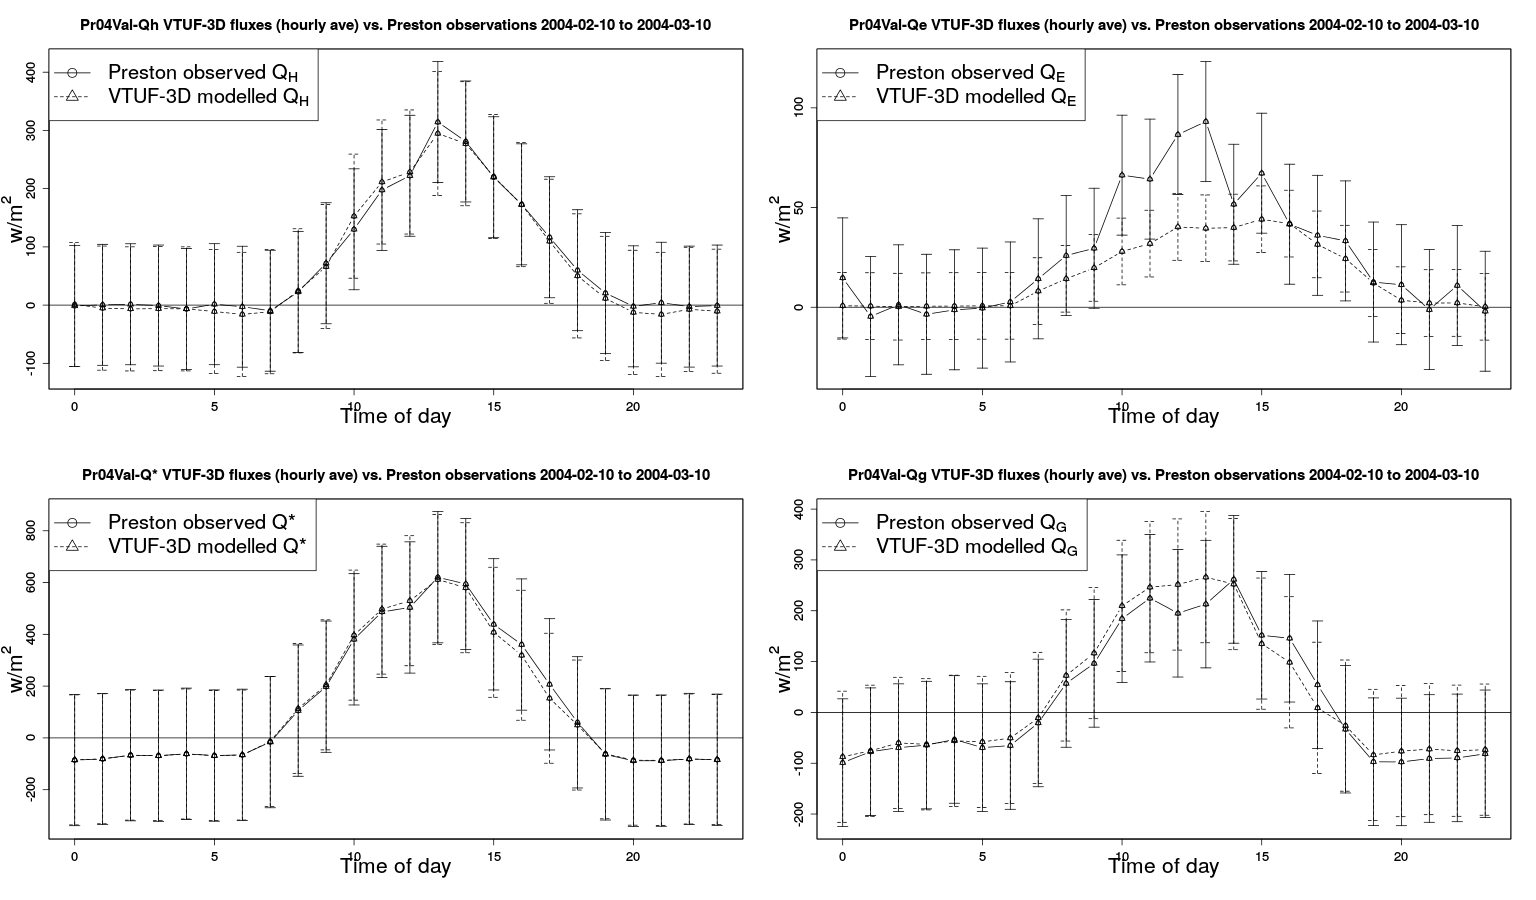
\includegraphics[trim = 0mm 0mm 0mm 0mm, clip, scale=0.30]{images/Pr04Val-EnergyBalanceOverallAve4Plots_.png}
\caption{Pr04Val run 30 day hourly average VTUF-3D flux comparisons to Preston flux observations for the period 10 February-10 March 2004, with error bars standard deviations. \label{fig:Preston30Day4} }     
\end{figure}



In a comparison of the 30 day monthly hourly averages, daily observed values of $Q_{H}$ peak at 314 W m$^{-2}$ compared to modelled values of 294 W m$^{-2}$ for the Pr04Val scenario. For the other fluxes, $Q_{E}$, $Q^{*}$, and $Q_{G}$, peaking observed vs. modelled values are 93 vs. 40, 621 vs. 612, and 213 vs. 266 W m$^{-2}$ respectively. The d, index of agreement (in which 1 indicates perfect agreement and 0 no agreement), for the Pr04Val evaluation (Figure \ref{fig:Preston6error}) shows d values of 0.964, 0.652, 0.998, and 0.957 for $Q_{H}$, $Q_{E}$, $Q^{*}$, and $Q_{G}$ respectively. RMSE (W m$^{-2}$) values are seen of 40.2, 33.1, 19.0,and 52.5. MBE (W m$^{-2}$) values are seen of -4.0, -9.5, 3.0, and -8.3. 

\begin{figure}[!htbp]
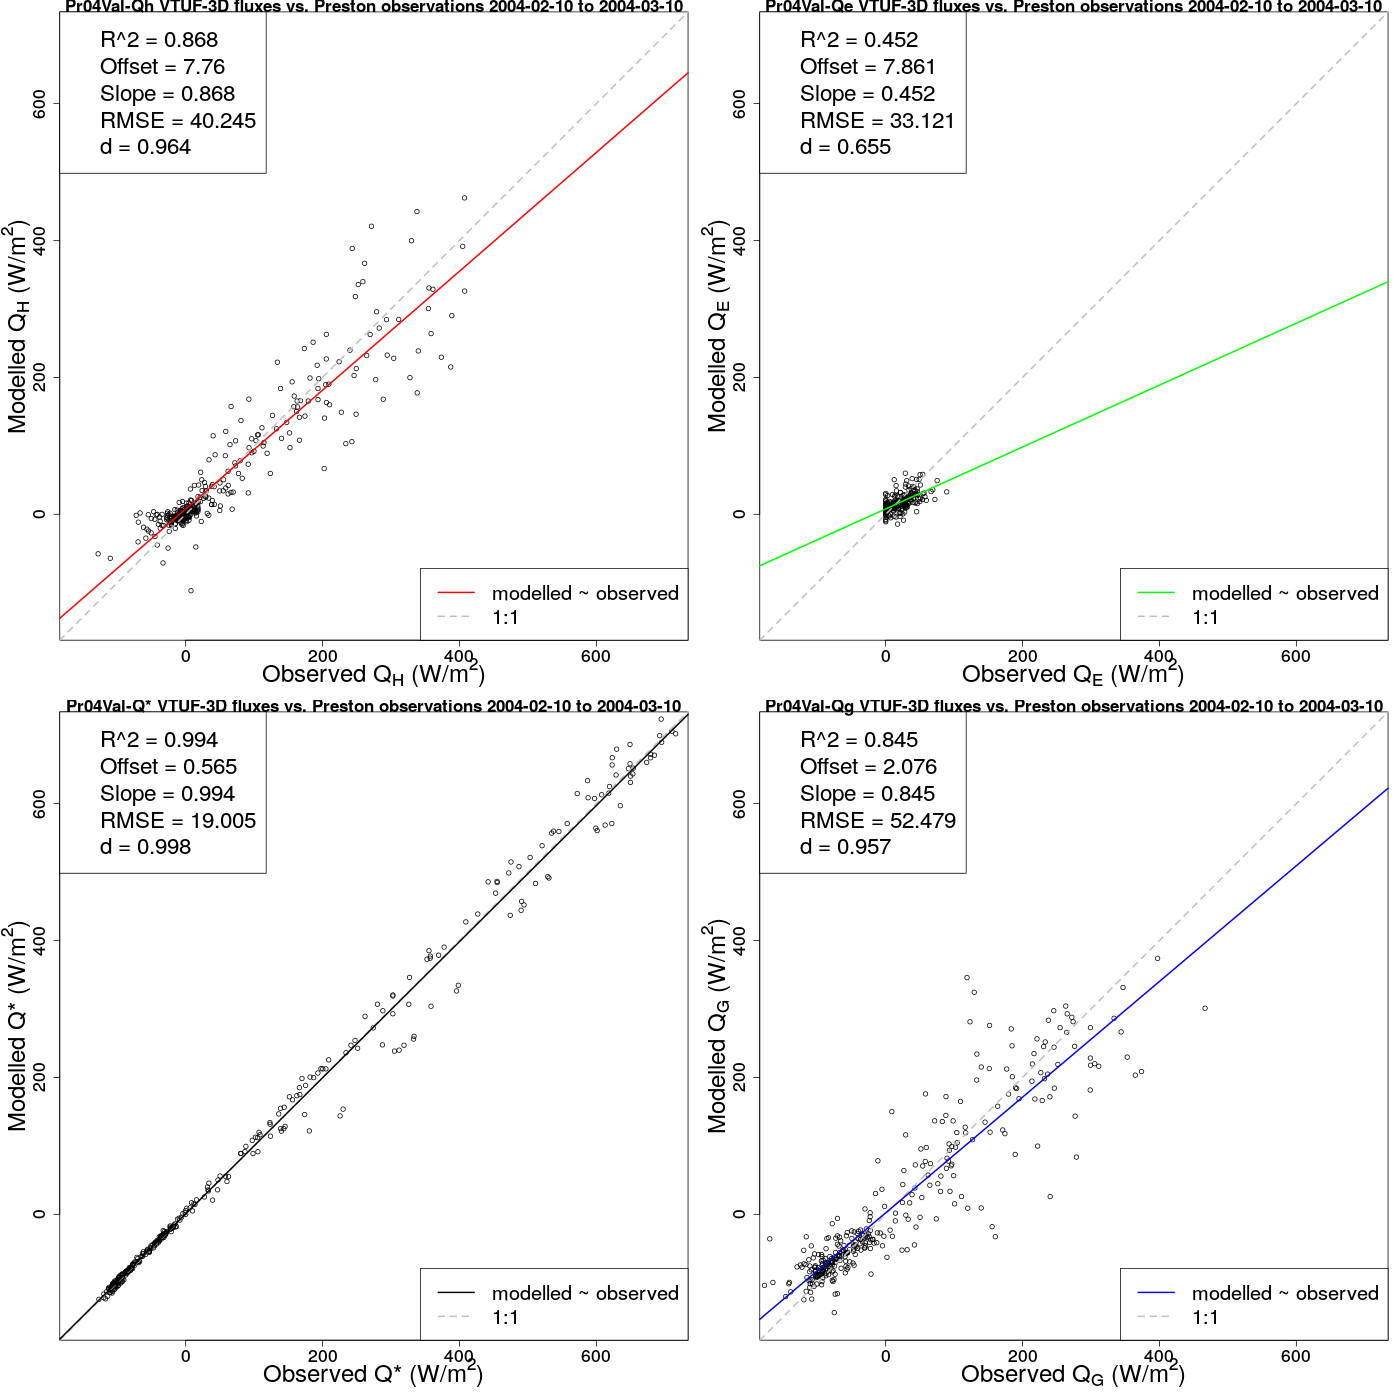
\includegraphics[trim = 0mm 0mm 0mm 0mm, clip, scale=0.30]{images/Pr04Val-ErrorPlots.png}
\caption{Pr04Val scenario modelled vs. observations for $Q_{H}$, $Q_{E}$, $Q^{*}$, and $Q_{G}$ fluxes for the period 10 February-10 March 2004. \label{fig:Preston6error}}   
\end{figure}

Figure \ref{fig:Prestonnoveg30day} presents a 30 day hourly average of both the Pr04Val and Pr04NoVeg scenarios with Pr04Val showing a much closer fit for all fluxes over a diurnal cycle. Figure \ref{fig:Prestonnovegerror} shows each component of the surface energy balance for the no vegetation scenario (Pr04NoVeg). These values show an improvement over the unimproved VTUF-3D model. The unimproved model yields results of d of 0.906, 0.0, 0.989, and 0.877, RMSE (W m$^{-2}$) of 87.0, 47.1, 51.6, 75.9, and MBE (W m$^{-2}$) of -6.3, 23.8, 41.1, 11.0 for $Q_{H}$, $Q_{E}$, $Q^{*}$, and $Q_{G}$ respectively. With the unimproved model, $Q_{H}$ is significantly over-predicted during the afternoon and under-predicted in the evenings. Flux $Q_{G}$ is under-predicted during the afternoons. Finally, $Q_{E}$ is not implemented in the model, so cannot be predicted at all. 

\begin{figure}[!htbp]
{\scriptsize a)} 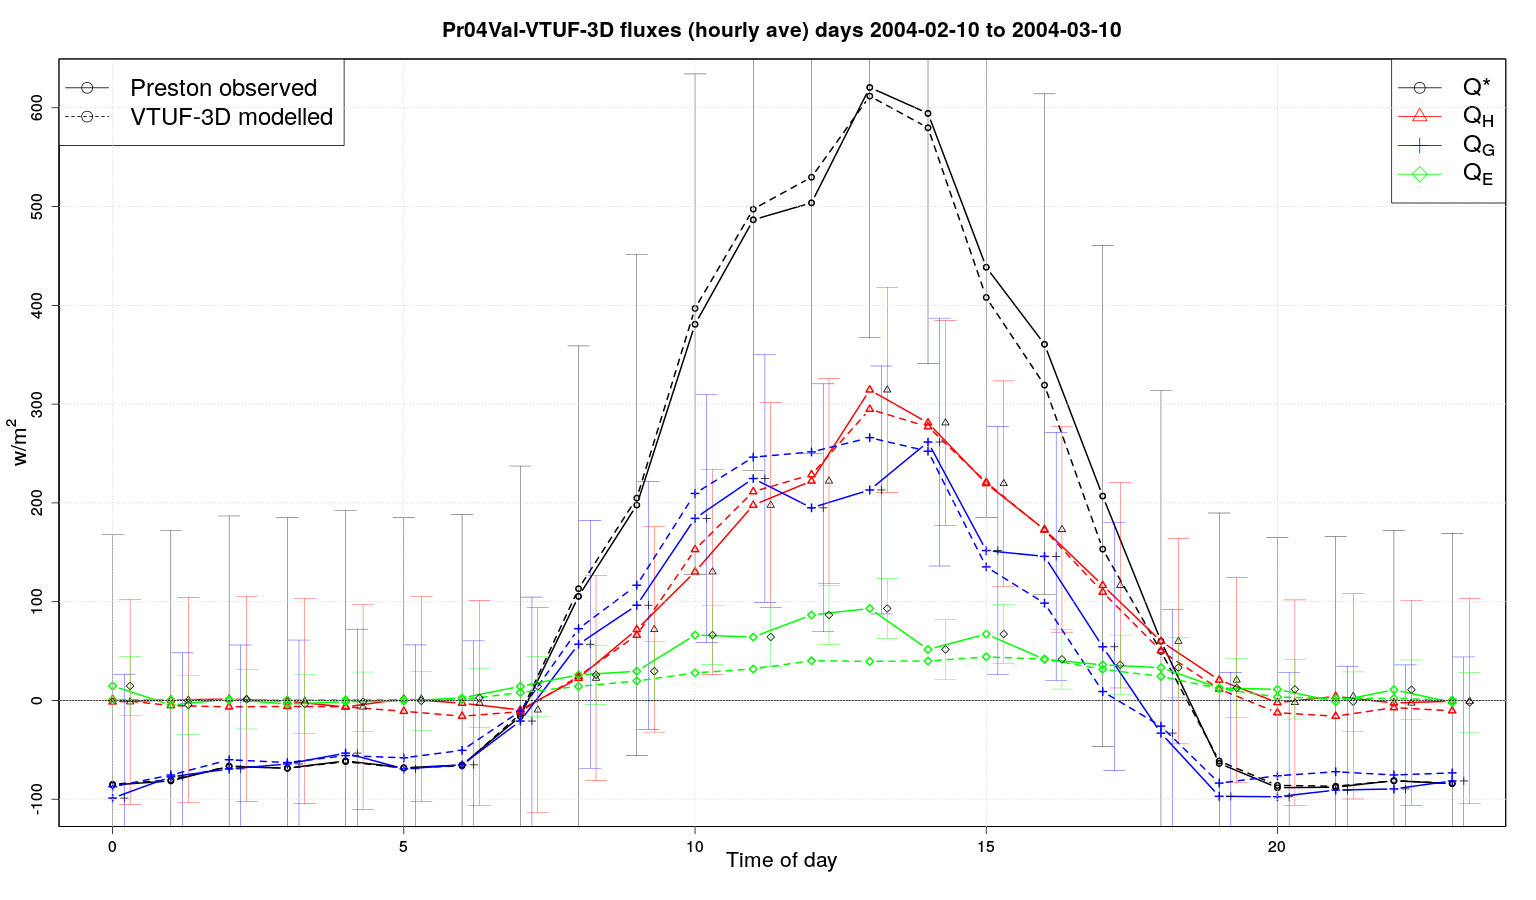
\includegraphics[trim = 0mm 0mm 0mm 0mm, clip, scale=0.16]{images/Pr04Val-EnergyBalanceOverallAve_.png}
{\scriptsize b)} 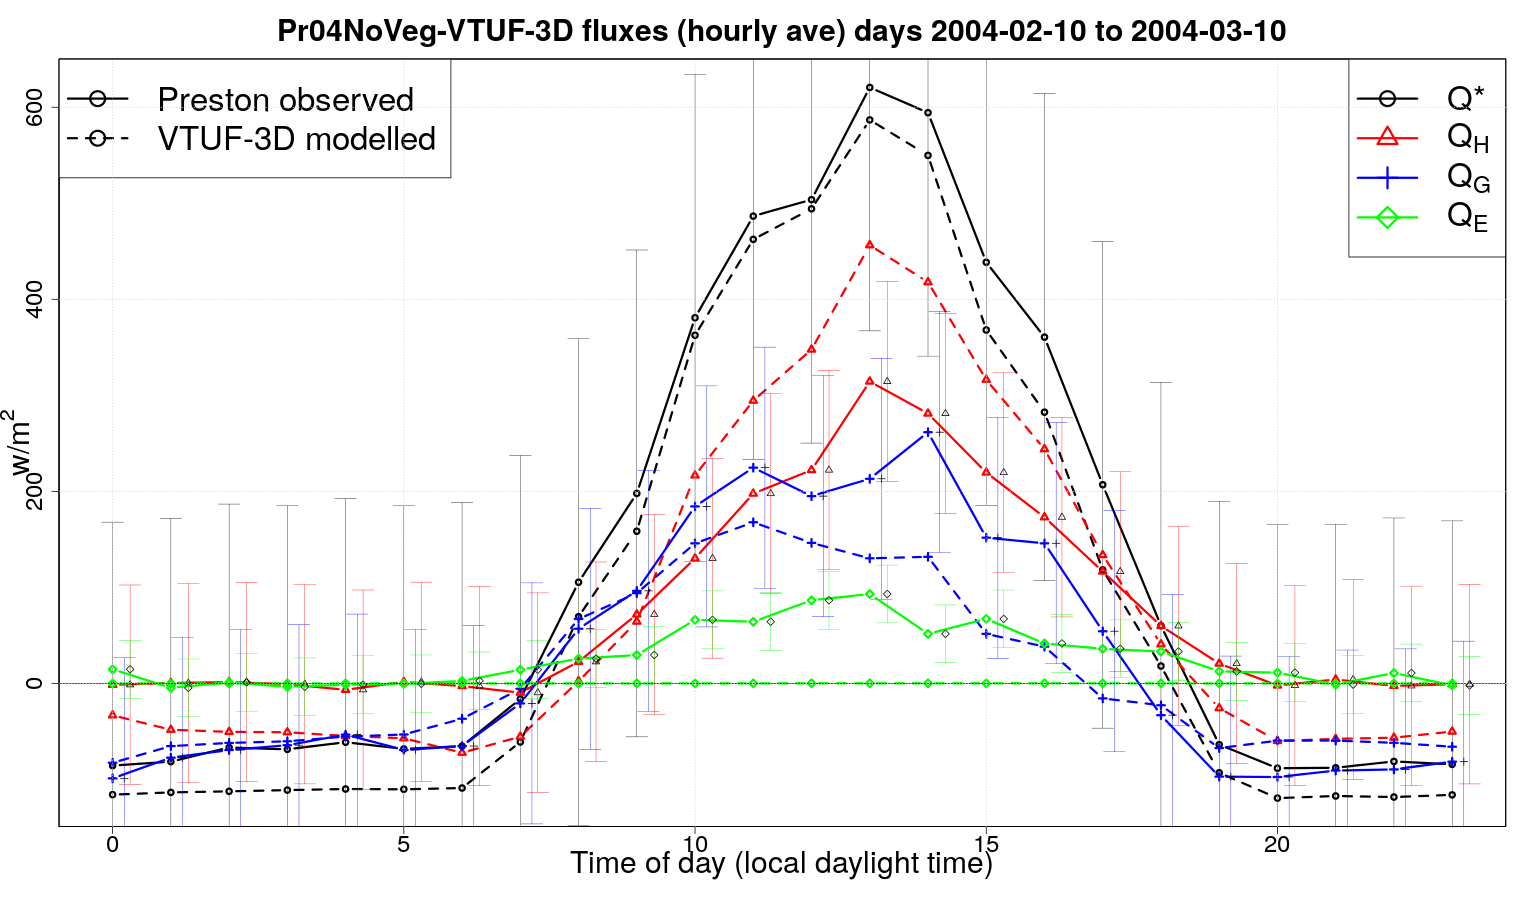
\includegraphics[trim = 0mm 0mm 0mm 0mm, clip, scale=0.16]{images/Pr04NoVeg-EnergyBalanceOverallAve_.png}
\caption{a) Pr04Val and b) Pr04NoVeg scenarios. 30 day hourly average VTUF-3D flux comparisons to Preston flux observations for the period 10 February-10 March 2004, with error bars observations standard deviations. \label{fig:Prestonnoveg30day}}    
\end{figure}

\begin{figure}[!htbp]
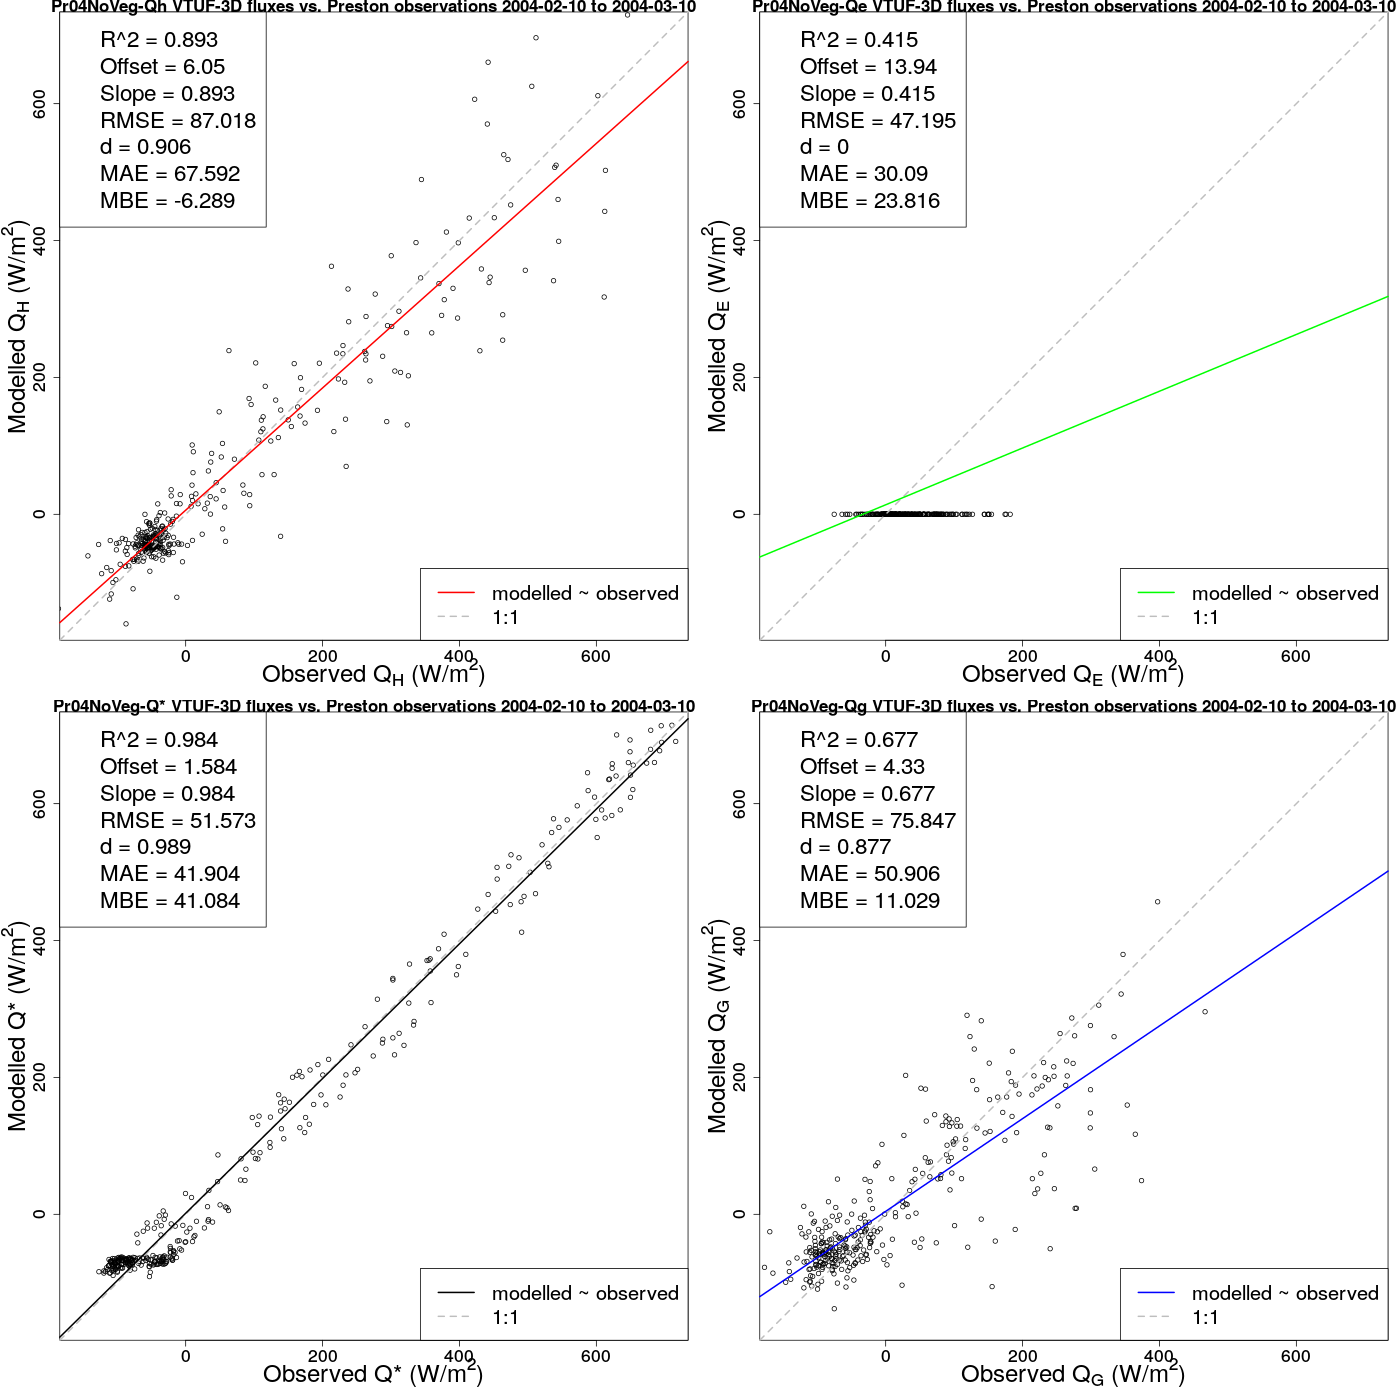
\includegraphics[trim = 0mm 0mm 0mm 0mm, clip, scale=0.30]{images/Pr04NoVeg-ErrorPlots.png}
\caption{Pr04NoVeg scenario modelled vs. observations for $Q_{H}$, $Q_{E}$, $Q^{*}$, and $Q_{G}$ fluxes for the period 10 February-10 March 2004. \label{fig:Prestonnovegerror}}    
\end{figure}

As an extension to the TUF-3D model, the addition of vegetation and associated $Q_{E}$ fluxes to VTUF-3D have created a large improvement to the model. The results of the intercomparison project \citep{Grimmond2011,Best2012} showed that land surface modelling schemes that include vegetation perform better than those that do not. In addition, schemes that integrate vegetation perform better than those who use a tiling method that treats the urban canyon and vegetation separately. Another important result from this intercomparison project was that $Q_{E}$ is the least well modelled flux across a range of urban land surface modelling schemes \citep{Grimmond2010}. Even the SUEWS model, which includes vegetation, as well as a very complete urban hydrology, tends to under-estimate $Q_{E}$ fluxes during day-time \citep{Jarvi2011}.




Using the RMSE and MBE values for fluxes $Q^{*}$, $Q_{H}$, $Q_{G}$ from Phase 4 of the Intercomparison project, the performance of the Pr04NoVeg scenario (as well as the Pr04NoVeg scenario) can be compared against the performance of 24 other urban land surface models. The RMSE and MBE values are taken from Figure 2 of \cite{Best2012}, for the Feb/Mar period, corresponding to the period for which the evaluation scenarios were run. A comparison of these Intercomparison MBE and RMSE results vs. modelled results is shown in Table \ref{fig:prestonrmse}. In the Phase 4 comparisons, for all fluxes, models with integrated vegetation had the lowest RMSE values (and \cite{Grimmond2011} found that models without vegetation were among the poorest performers). These were followed by tiled vegetation models while models without vegetation had the highest values. In comparison, the VTUF-3D Pr04Val scenario had lower RMSE values for all fluxes except $Q_{E}$ than each of the Phase 4 three model categories. For $Q_{E}$, the VTUF-3D scenario Pr04Val performed better than the no vegetation category, but with slightly higher errors than the tiled and integrated categories. In terms of absolute differences between RMSE values for the best performing Intercomparison model category, Pr04Val scenario RMSE values differed by -6, -5, -25, and 7 W m$^{-2}$ for $Q^{*}$, $Q_{H}$, $Q_{G}$, and $Q_{E}$ respectively. In MBE values, VTUF-3D performed better for $Q_{H}$ and $Q_{G}$ in all categories, better than the tiled and integrated categories with $Q^{*}$, and better for $Q_{E}$ in the no vegetation category.


 \begin{center}
 \begin{table}[!htbp]
 \caption{RMSE (W m$^{-2}$) and MBE (W m$^{-2}$) statistics VTUF-3D vs. Intercomparison \citep{Best2012} comparison for Preston evaluation scenarios for 10 February-10 March 2004.\label{fig:prestonrmse}} 
 \begin{tabular}{  | l | l | l|l|l| } 
 \hline \textbf{Scenario name} &\textbf{$Q^{*}$}& \textbf{$Q_{H}$}& \textbf{$Q_{G}$}& \textbf{$Q_{E}$}  \\ \hline
 Pr04Val RMSE & 19.0&	40.2&	52.5&	33.1    \\ \hline
   Pr04Val MBE & 3.0&	-4.0&	-8.3&	-9.5    \\ \hline
 Pr04NoVeg RMSE & 51.6&	87.0&	75.9&	47.1  \\ \hline	
   Pr04NoVeg MBE & 41.1&	-6.3&	11.0&	23.8  \\ \hline	
 IntercomparisonNoVeg RMSE & 40&	105&	85&	38   \\ \hline
   IntercomparisonNoVeg MBE & 2&	45&	-16& -32   \\ \hline
 IntercomparisonTiled RMSE &  27&	60&	77&	25  \\ \hline
   IntercomparisonTiled MBE & -7&	13&	-22& -1  \\ \hline
 IntercomparisonIntegrated RMSE & 25&	45&	77&	26   \\ \hline
   IntercomparisonIntegrated MBE & -5&	13&	-18& -3   \\ \hline
 
   \end{tabular} 
 \end{table}
 \end{center} 
 

This project uses an innovative method, the first time vegetation has been tiled and incorporated into a micro-scaled surface energy balance model in this manner. This method was anticipated to bring performance improvements over the previous version of the model that did not consider vegetation. The results suggest that this is the case, shown in the the results of the Pr04NoVeg no vegetation evaluation scenario. In comparisons with other urban models, VTUF-3D has shown comparable performance to these other urban models (while delivering micro-scaled results). In addition to the improved modelling performance, the addition of vegetation modelling has dramatically improved the applicability of VTUF-3D to a wide range of modelling problems. Indeed, without this addition, the main aim of this model, to determine the thermal comfort improvements due to urban vegetation and water, would not be possible. 

Despite these improvements to the modelling tool, the fluxes of $Q_{E}$ show some divergences from the observations. These divergences were anticipated as there are three current limitations of VTUF-3D that can account for low $Q_{E}$ levels that need addressing in future versions of the model. The first limitation is not accounting for precipitation on impervious surfaces. Many spikes of $Q_{E}$ fluxes are seen in the observations shortly after rainfall. \cite{Demuzere2014} found evaporation from impervious surfaces in urban areas after rainfall can contribute to an approximately 10\% increase of $Q_{E}$ over a two month period, while \cite{Wouters2013} found increases of 45 W m$^{-2}$ in $Q_{E}$ for up to 12 hours of daylight following rainfall. In other parameters, there is evidence that wet impervious surfaces can have some other short term cooling impacts. \cite{Hendel2016} observed that hourly watering of urban pavement during heat wave conditions could deliver maximum air temperature reductions (at 1.5m above ground level) of 0.79 \SI{}{\degreeCelsius} as well as $T_{mrt}$ and UTCI reductions of 1.67\SI{}{\degreeCelsius} and 1.03\SI{}{\degreeCelsius} respectively. While this last study might indicate an upper bound to the impact of wet pavement, until this portion of precipitation received is accounted for in the model, care should be taken when modelling periods that contain precipitation.

The second limitation is not accounting for irrigation. While Melbourne was under Stage 2 water restrictions during the observation/modelling period \citep{MelbourneWater2016a}, there would have been some amount of irrigation occurring to contribute to greater observed $Q_{E}$ fluxes than modelled. Estimates of household irrigation during February 2004 are of frequencies of 2.8 times a week (3.1 for only the homes which irrigate) with average irrigation flows of 16.3slm and average durations of 46 minutes per irrigation event \citep{Roberts2005}. Irrigation is an important limitation that needs addressing as quantifying the benefits of irrigation as part of WSUD is another intended use of this model. 

The third limitation is the full diversity of vegetation and trees of the modelled area are not represented in the modelled domain. In this study, parametrisations were included for grass and two evergreen tree species. However, the number of vegetation parametrisations is not a limitation in the model itself, as any type of vegetation can be plugged into the model. To overcome this deficit, more work needs to be done. Completion of each parametrisation is a time consuming process requiring numerous observations of tree physiology specifications, or specifying parameters from the literature. A standard limitation of many empirical models requiring a choice of either deciduous or evergreen vegetation does not exist in the model itself as these new vegetation types can include either, as long as the proper observations and parametrisations are completed on each type.


Another consideration is that the under-prediction of $Q_{E}$ is likely contributing to the over-estimating of $Q_{G}$ (calculated as a residual in MAESPA vegetation tiles). An improvement in modelling of the $Q_{E}$ fluxes will likely lead to an improvement in the modelled $Q_{G}$ fluxes. Finally, values of $Q_{F}$, anthropogenic heat (W m$^{-2}$), are not accounted for in the VTUF-3D model, but that do contribute to the total $Q_{H}$ fluxes in the observations. Flux values for this modelling and observation period (summertime) are anticipated to contribute peaks of over 15 W m$^{-2}$ for low density areas of cities and peaks of 30-60 W m$^{-2}$ for medium density areas \citep{Sailor2004}. In both the observations and modelling results, these unaccounted fluxes will be present in the errors for the four observed and modelled fluxes. 



%There will remain an amount of uncertainty in comparing the modelled results to the observations because of inherent uncertainties to both approaches. The observations were collected via a flux tower at 40m height, above the height of the urban roughness sublayer. The modelled results are the average of the fluxes from all of the urban surfaces, within the urban canyon and well within the urban roughness sublayer. While these comparisons can be done, i.e. \cite{Grimmond2011}, there remains an amount of uncertainly as they are comparing two slightly different values. However, tests were performed (not presented here) and found the model conserved energy despite different sources of modelled fluxes.


%%%%%%%%%%%%%%%%%%%%%%%%%%%%%%%%%%%%%%%%%%%%%%%%%%%%%%%%%%%%%%%%%%%%%%%%%%%%%%%%%%%%%%%%%%%%%%%%%%%%%%%

\subsection{Spatial and temporal mean radiant temperature and human thermal comfort index evaluation}\label{sec:CoMValidations}

While evaluating against the Preston flux observations indicates that VTUF-3D performs well in partitioning the basic energy fluxes, there are a number of other aspects that need to be evaluated. Given the intended application of the model to assess the impacts of urban greening on HTC at a micro-climate scale, a demonstration of accurate predictions of $T_{mrt}$ and HTC indices is an important step. Both parameters are highly influential on thermal comfort and capture the effects of varied shading across an urban canyon. Observational studies have shown that street orientation, tree placement on the street, and canopy cover amounts can cause large micro-climate variations in HTC and of $T_{mrt}$ \citep{Sanusi2016,Oliveira2011,Ali-Toudert2007}. The evaluation will be performed by comparing predicted spatial values of $T_{mrt}$ and UTCI to observed values. Note, evaluations of spatial air temperature ($T_{a}$) will not be possible as VTUF-3D only predicts air temperature as a single canyon-wide value and not spatially.

\subsubsection{George St. and Gipps St. dataset overview}
This set of evaluations was undertaken using observations from George St. and Gipps St. in the City of Melbourne \citep{Coutts2015}. Observations were taken at a number of observation stations, recording air temperature, wind speed, humidity, and incoming short wave radiation, located along the two streets. The purpose of the study was to observe and quantify the effects of street trees on HTC and recorded observations in streets with varied canopy cover. Figure \ref{fig:GeorgeGippsSt2} shows the two streets used in this evaluation. 

\begin{figure}[!htbp] 
\center
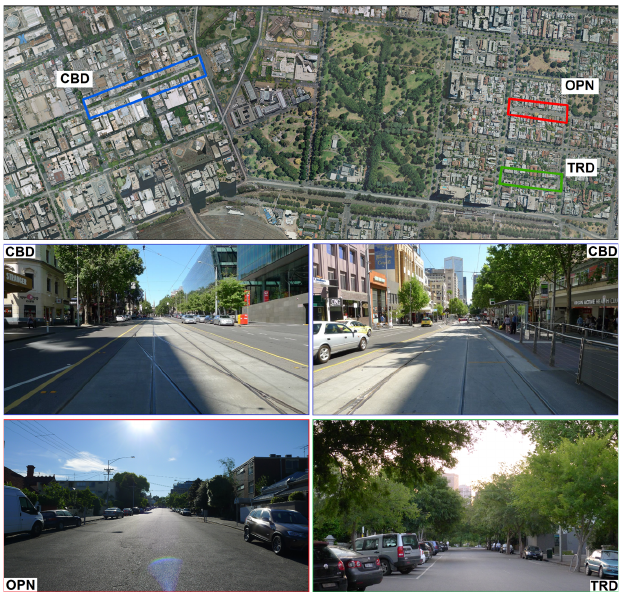
\includegraphics[trim = 60mm 95mm 0mm 0mm, clip, scale=1.0]{{images/GippsGeorgeImages(Coutts2015p58).png}} ~
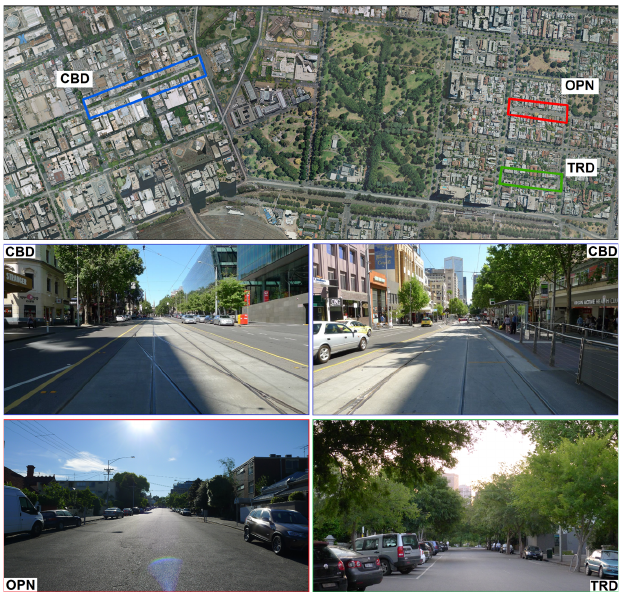
\includegraphics[trim = 0mm 0mm 0mm 112mm, clip, scale=1.0]{{images/GippsGeorgeImages(Coutts2015p58).png}} ~
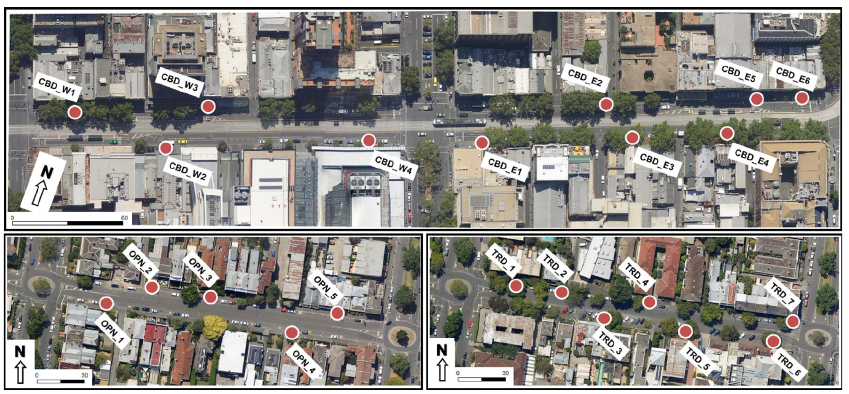
\includegraphics[trim = 0mm 0mm 0mm 64mm, clip, scale=0.73]{{images/GippsGeorgeImages2(Coutts2015p58).png}} ~
 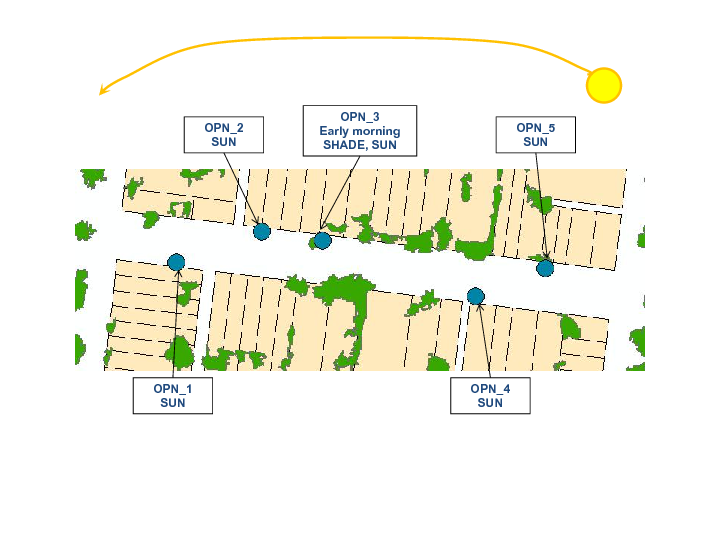
\includegraphics[trim=30mm 35mm 25mm 5mm, clip, scale=0.35]{images/CoMLocations-0.png}
~
 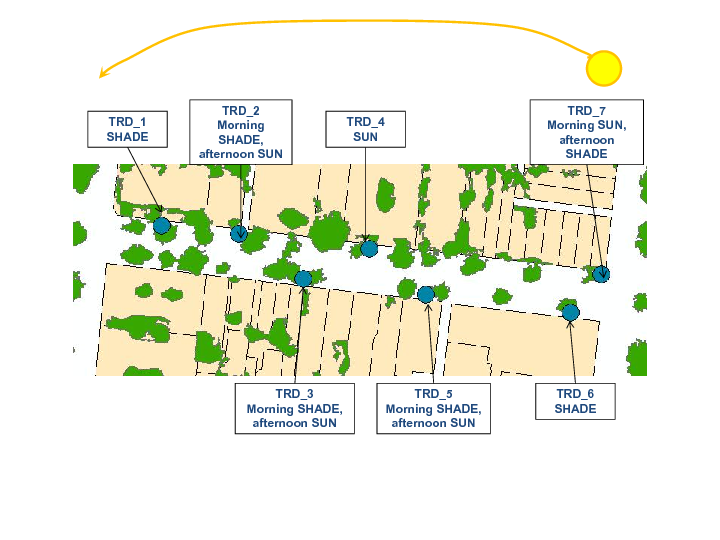
\includegraphics[trim=30mm 35mm 25mm 5mm, clip, scale=0.35]{images/CoMLocations-1.png}
\caption{Location and photos of each street: Gipps St. (OPN), and George St. (TRD). Aerial view of the streets highlighting individual station locations and tree canopy coverage in Gipps St. (OPN), and George St. (TRD) \citep[p.58]{Coutts2015}.\label{fig:GeorgeGippsSt2}} 
\end{figure}

The two streets both have a shallow urban canyon, characterised as LCZ6B (open low-rise) \citep{Stewart2012b}, and both are orientated E-W. Gipps St. contains a very limited canopy cover and is designated open (OPN) in the observation study. George St. contains a dense canopy cover and is designated as treed (TRD). Some of the sensors were placed directly under tree canopies and others out in the open. A main purpose of the VTUF-3D model will be to evaluate the impacts of different arrangements urban vegetation on HTC in urban canyons. Differing amounts of canopy cover are a major factor of these different arrangements. Because of this, an evaluation using observations from two very similar streetscapes which mainly differ in the amount of canopy cover will be an ideal evaluation of VTUF-3D's spatial accuracy in resolving the impacts of different arrangements and quantities of urban greenery on HTC.

Tree cover of Gipps St consists of \textit{Ulmus parvifolia} (Chinese Elm) with median heights of 9.5m and crown diameters of 9.6m. The limited tree cover of George St. also consists of \textit{U. parvifolia}. The entire street canyon floor of both streets are impervious, consisting of concrete and asphalt, with the exception of a small pervious area of 1.2m$^{2}$ surrounding each tree in the road areas. General characteristics of the two sites are summarised in Table \ref{tab:comvalpara}.

\begin{table}[!htbp]
\caption{Gipps/George St. evaluation site characteristics \citep{Coutts2015}. \label{tab:comvalpara}}     
\begin{tabular}{| l | l |l|}
\hline
\textbf{Property} & \textbf{Gipps St. (OPN)} & \textbf{George St. (TRD)} \\ \hline
Observation stations & 5 & 7\\ \hline
Minimum building height (m) & 4 & 4\\ \hline
Maximum building height (m) & 14 & 11\\ \hline
Average building height (m) & 7 & 8 \\ \hline
Street width (m) & 25 & 25 \\ \hline
Mean H:W & 0.27 & 0.32 \\ \hline
Plan area canopy cover (\%) & 12 & 45 \\ \hline

\end{tabular}
\end{table}

Observations were taken at heights of 3.5 to 4.0m on existing light poles at locations indicated in Figure \ref{fig:GeorgeGippsSt2}. The observation period was for 21 months, from October 2011 to June 2013. Each observation station recorded air temperature, wind speed, humidity, incoming shortwave, and black globe temperature. For each station, mean radiant temperature was calculated using a formula of \cite{Kantor2011} (a slight variation of the equation used in this study, in Section \ref{sec:tmrtutci}). UTCI was calculated using RayMan Pro 2.1 \citep{Matzarakis2010} for a 35 year old male, clothing factor of 0.9, and activity rate of 80 W. This temperature was then compared to \cite{Brode2012a} assessment scale of thermal stress.

Station locations (noted on Figure \ref{fig:GeorgeGippsSt} as yellow pins and red dots on Figure \ref{fig:GeorgeGippsSt2}) are shown in the modelled domains for both streets. Stations for George St. are referred to as TRD\_2, TRD\_3, TRD\_4, and TRD\_5  (also known as EM12, EM9, EM3, and EM2 on Figure \ref{fig:GeorgeGippsSt}). Stations for Gipps St. are referred to as OPN\_3, OPN\_4, OPN\_5 (also known as EM5, EM11, and EM8). Table \ref{tab:georgegippsvf} shows sky view factor (SVF) resulting from buildings and trees at each observation site.

% I understand why you have done this. I renamed those stations (from EMxx) in the paper for clarity... 

%A question could be asked as to why they are named EMxx here? It could confuse the reader.... Annoying, but you should probably stick to the TRD and OPN labels....

\begin{figure}[!htbp]
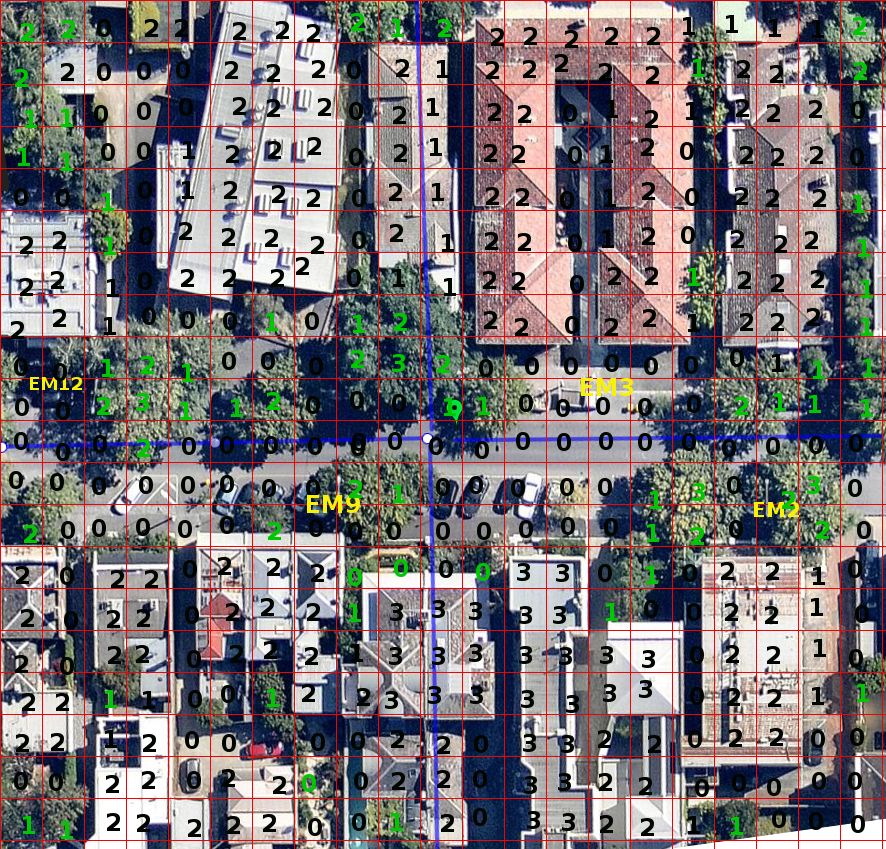
\includegraphics[trim = 0mm 0mm 0mm 0mm, clip, scale=0.33]{{images/GeorgeSt-100x100m-5m_grid_heights.png}}~
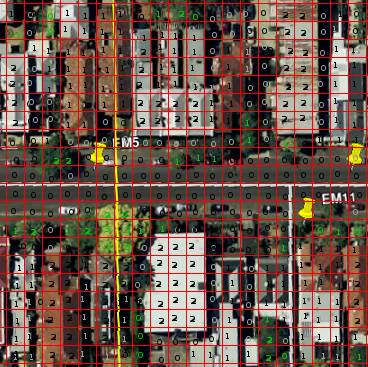
\includegraphics[trim = 0mm 0mm 0mm 0mm, clip, scale=0.78]{{images/Gipp200x200_5mgrid_heights.png}}
\caption[George St/Gipps St - Modelled domains with 4 and 3 observation stations located on street]{George St/Gipps St - Modelled domains with 4 and 3 observation stations located on street.\label{fig:GeorgeGippsSt}}  
\end{figure}

\begin{center}
\begin{table}[!htbp]
\caption{George St./Gipps St. observation station sky view factors \citep{Coutts2015}.\label{tab:georgegippsvf}}
  \begin{tabular}{  | c|c|c | c |  } 
	\hline \textbf{Observation point}  & \textbf{Total SVF} & \textbf{Build. SVF}& \textbf{Trees SVF} \\ \hline
	OPN\_3 & 0.63  & 0.81  & 0.18    \\ \hline
	OPN\_4& 0.86 & 0.94  & 0.08    \\ \hline
	OPN\_5 & 0.77  & 0.78  & 0.01   \\ \hline
    TRD\_2& 0.22  & 0.85  & 0.63    \\ \hline
	TRD\_3 & 0.17  & 0.70  & 0.53    \\ \hline
	TRD\_4 & 0.66  & 0.81  & 0.15   \\ \hline
	TRD\_5 & 0.18  & 0.71  & 0.53    \\ \hline
  \end{tabular} 
\end{table}
\end{center} 


These domains were configured accordingly using a 100x100m subset of the two streets (Figure \ref{fig:GeorgeGippsSt}). Simulations were run for both streets for the period 1 February 2014 to 1 March 2014 with a domain resolution of 5m grids. Building heights and locations and vegetation location and heights for both streets are shown in Figure \ref{fig:GippsStConfig}. Model parameters were set to the values given in Table \ref{tab:modcomvalpara}. Most of these values are TUF-3D default values, from \cite{Krayenhoff2007}. Vegetation settings for the mix of two tree types (olive and brushbox) as well as grass are set to the values given in the model design vegetation parametrisation section (\ref{sec:maespavegpara}).

\begin{figure}[!htbp]
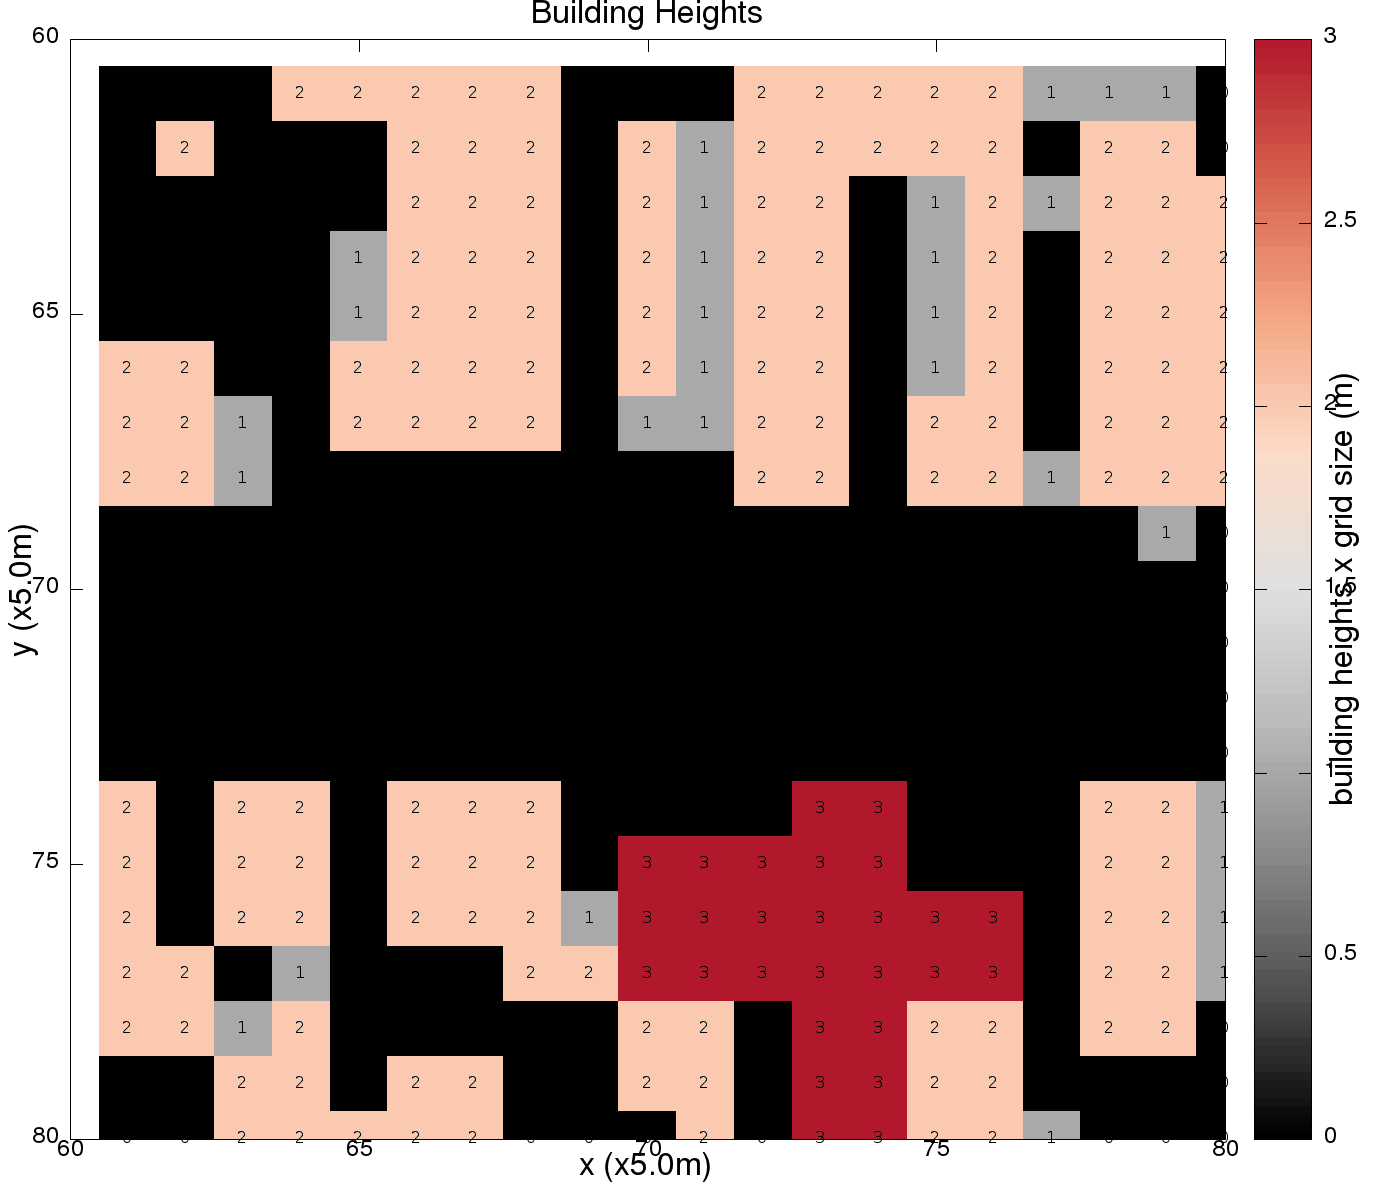
\includegraphics[trim = 0mm 0mm 0mm 0mm, clip, scale=0.20]{{images/GeorgeValidationCentralBuildingHeights.png}}~
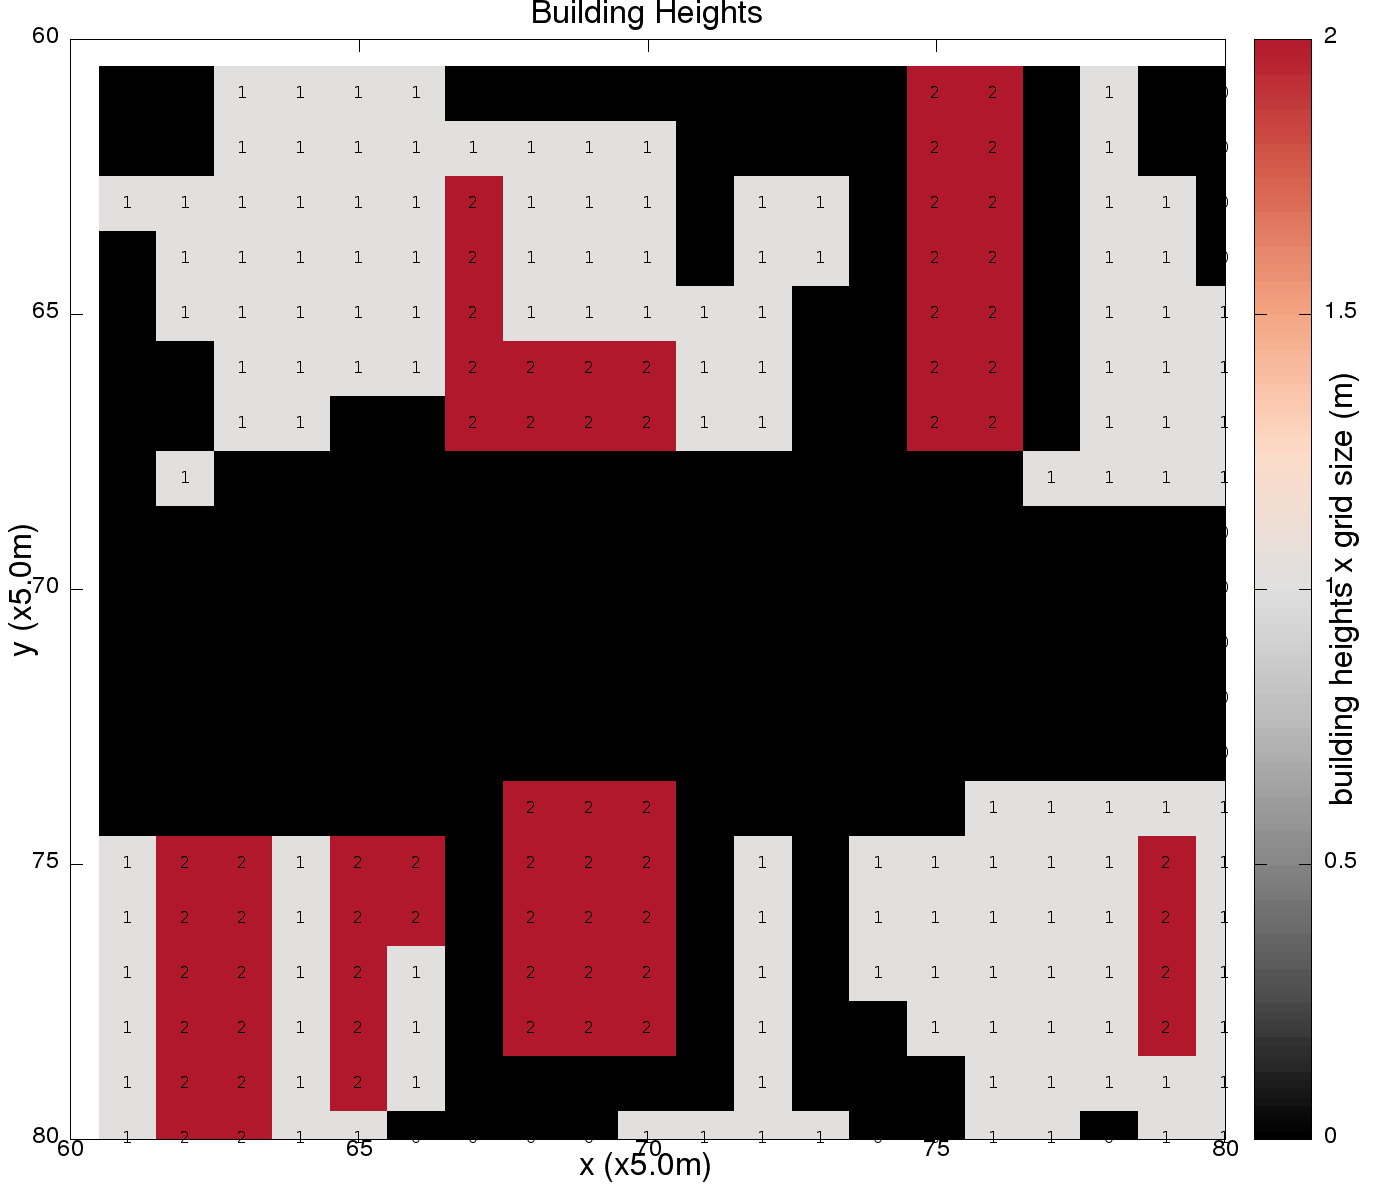
\includegraphics[trim = 0mm 0mm 0mm 0mm, clip, scale=0.20]{{images/GippValidationCentralBuildingHeights.png}} \\
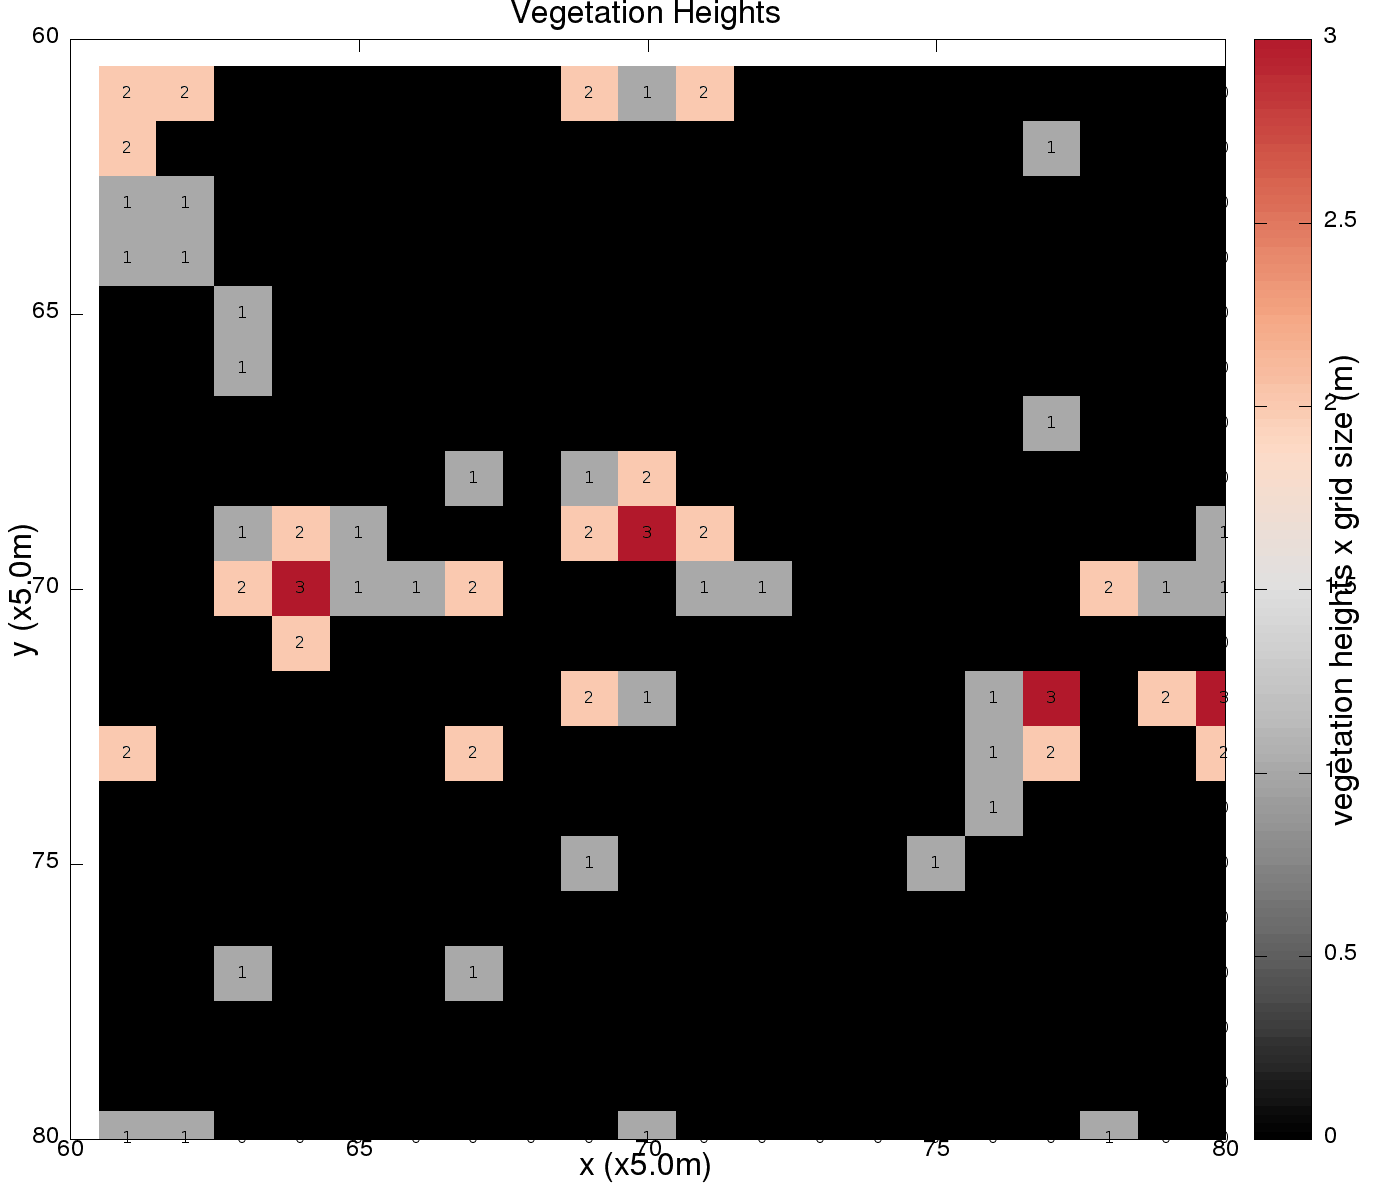
\includegraphics[trim = 0mm 0mm 0mm 0mm, clip, scale=0.20]{{images/GeorgeValidationCentralVegHeights.png}}~
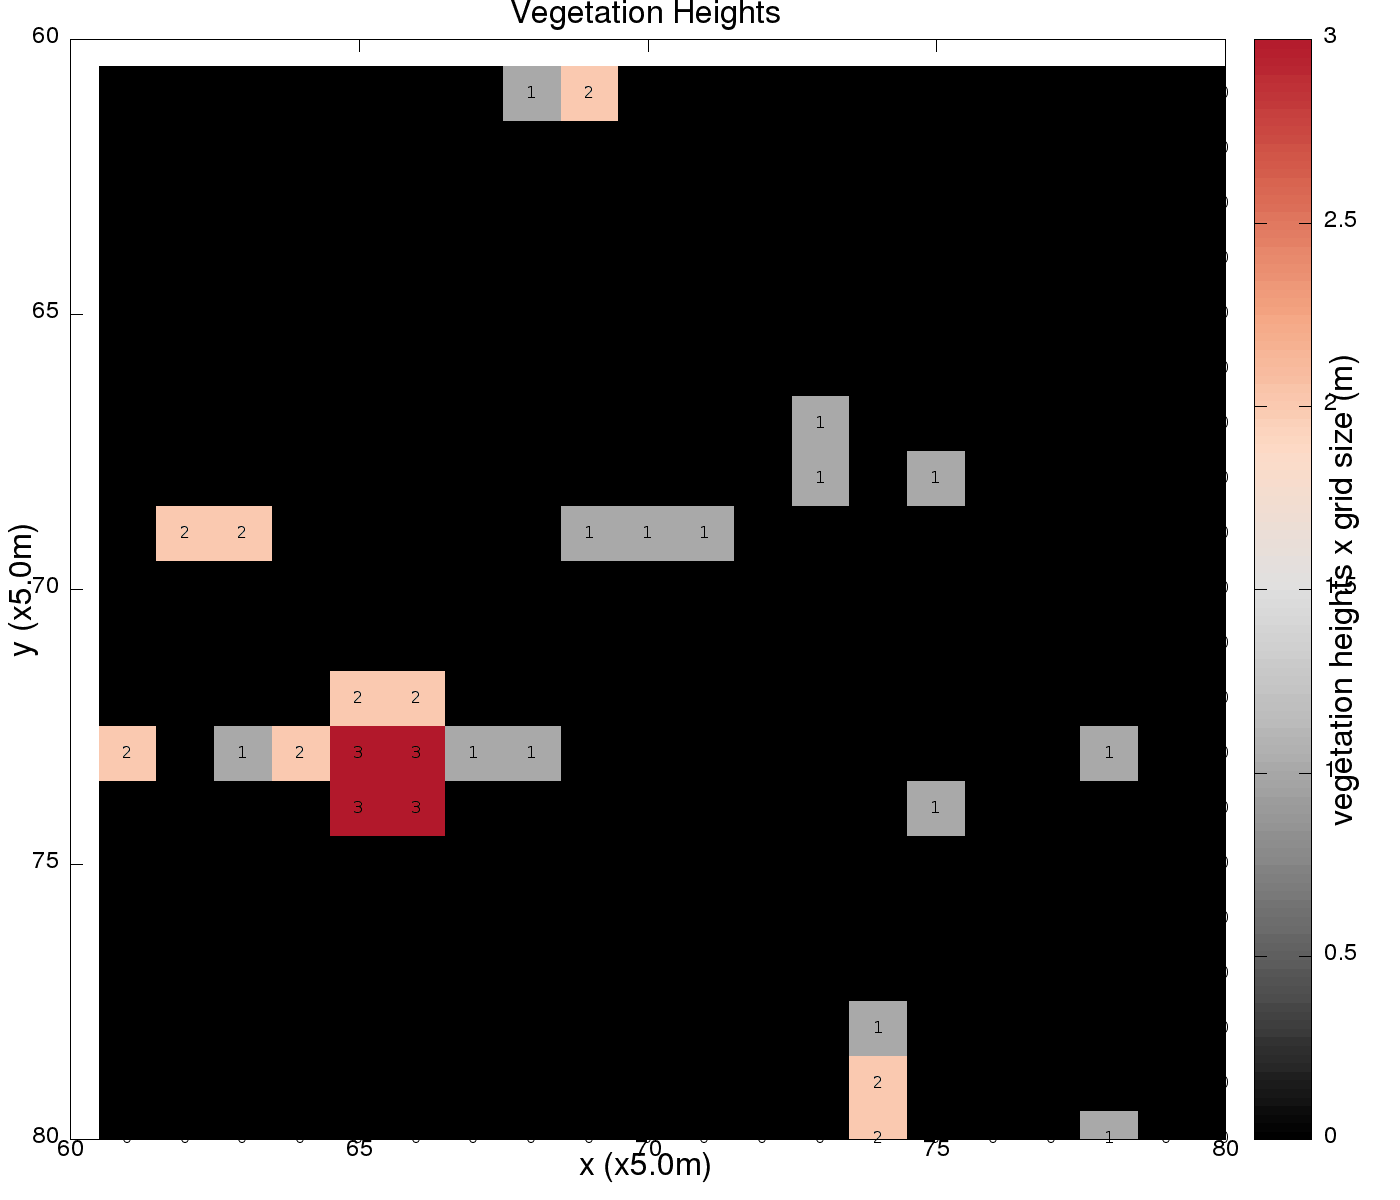
\includegraphics[trim = 0mm 0mm 0mm 0mm, clip, scale=0.20]{{images/GippValidationCentralVegHeights.png}}
\caption[Building heights (top) / Vegetation cover (bottom) - George St (left), Gipps St. (right)]{Building heights (top) / Vegetation cover (bottom) - George St (left), Gipps St. (right).\label{fig:GippsStConfig}}  
\end{figure}

\begin{table}[!htbp]
\caption{George/Gipps St. evaluation scenario model parameters. \label{tab:modcomvalpara}}     
\begin{tabular}{| p{8.0cm} | l | l|}
\hline
\textbf{Parameter} & \textbf{Value(s)}& \textbf{Source} \\ \hline
Albedo (roof, street, wall)   & 0.15, 0.10, 0.30 & \cite{Krayenhoff2007}   \\ \hline
Emissivity (roof, street, wall)   & 0.92, 0.92, 0.88 & \cite{Krayenhoff2007}   \\ \hline
Forcing data height (m)  & 4.0 & \cite{Coutts2015}   \\ \hline
Mean height of buildings, George St./Gipps St. (m)  & 9.4, 6.8  & Calculated from domain  \\ \hline
Mean height of trees, George St./Gipps St. (m)  & 7.45, 8.14  & Calculated from domain  \\ \hline
Initial $T_{sfc}$ (roof, street, wall) (\SI{}{\degree})  & 18.0, 23.0, 22.0  & \cite{Krayenhoff2007}  \\ \hline
Constant building internal air temperature (base of roofs and walls) (\SI{}{\degreeCelsius})  & 22.0, 20.0  & \cite{Krayenhoff2007}  \\ \hline
Constant deep-ground temperature (\SI{}{\degreeCelsius})  & 19.0 & \cite{Krayenhoff2007}  \\ \hline
Constant building internal floor temperature (\SI{}{\degreeCelsius})  & 15.0 & \cite{Krayenhoff2007}  \\ \hline
\end{tabular}
\end{table}

The two evaluation simulations (designated GeorgeValidation and GippsValidation) were run for 30 days between the dates 31 January 2012 and 1 March 2012, forced by the observations (of observation station OPN\_1) from \cite{Coutts2015} for those days. Values used from the observations include air temperature, wind speed, wind direction, and air pressure. Values for $L\downarrow$ are taken from Melbourne Airport observations (station 086282, Melbourne Airport) \citep{BOM2016b}. Values for $K\downarrow$ are taken from one minute solar observations (station 086282, Melbourne Airport) \citep{BOM2016}.  For full radiation vegetation runs, the mean global irradiance was used while for diffuse runs, the mean diffuse irradiance was used. In addition, the MAESPA FBEAM variable (fraction of incident PAR which is direct-beam) is set to 0.0 in the forcing data for diffuse runs. Values of CO$_{2}$ for vegetation forcing files were set to a constant of 450 ppm throughout the modelling period.


The period covered contains a range of conditions, as shown in Figure \ref{fig:CoMtemp}. The period especially features a number of hot days (over 30\SI{}{\degreeCelsius}). As one of the major applications of VTUF-3D will be examining high temperature moderation, evaluation over a period containing these hot days is important. This observation period contains no days with precipitation.


\begin{figure}[!htbp]
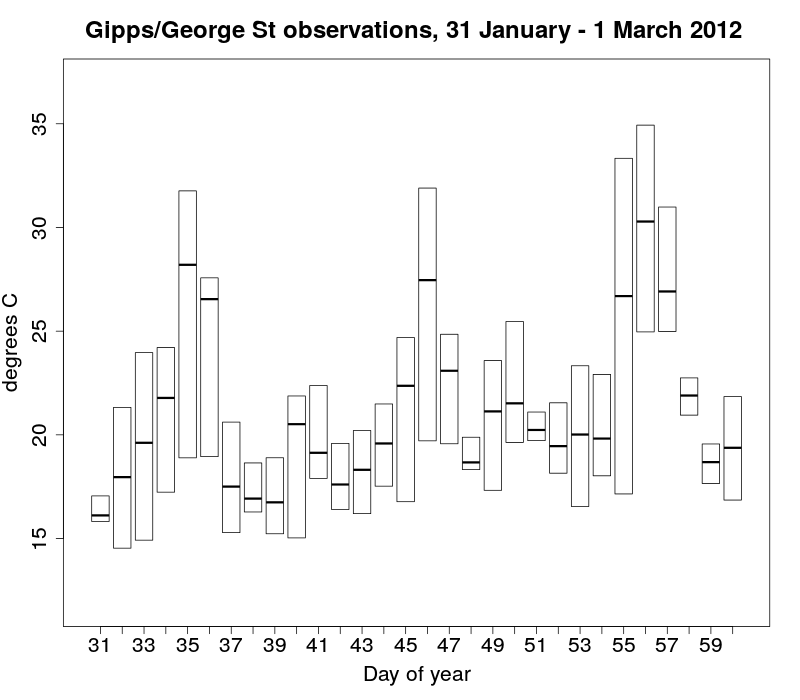
\includegraphics[trim = 0mm 0mm 0mm 0mm, clip, scale=0.30]{images/CoMTempFeb2012.png}
\caption{Daily maximum, minimum, and mean air temperature observations of Gipps/George St. during the evaluation period of 31 January - 1 March 2012.\label{fig:CoMtemp}} 
\end{figure}



\subsubsection{George/Gipps St. evaluation results}
%GeorgeValidation
%runDirectory=/home/kerryn/Documents/Work/VTUF-Runs/CoMValidations/GeorgeValidation
%Directories: /home/kerryn/Documents/Work/VTUF-Runs/CoMValidations/GeorgeValidation created
%2 runDirectory=/home/kerryn/Documents/Work/VTUF-Runs/CoMValidations/GeorgeValidation
%domain=/home/kerryn/Documents/Work/VTUF-Runs/CoMValidations/GeorgeValidation
%Tree height average=7.45
%Percentages: 
%Trees: 0.137
%Grass: 0.007
%Building: 0.495
%Streets: 0.361
%getWeatherData=GeorgeSt_EM10 2012 31 30

%runDirectory=/home/kerryn/Documents/Work/VTUF-Runs/CoMValidations/GippValidation
%Directories: /home/kerryn/Documents/Work/VTUF-Runs/CoMValidations/GippValidation created
%2 runDirectory=/home/kerryn/Documents/Work/VTUF-Runs/CoMValidations/GippValidation
%domain=/home/kerryn/Documents/Work/VTUF-Runs/CoMValidations/GippValidation
%Tree height average=8.14
%Percentages: 
%Trees: 0.067
%Grass: 0.022
%Building: 0.495
%Streets: 0.416
%getWeatherData=GeorgeSt_EM10 2012 31 30




The two scenarios GeorgeValidation and GippsValidation were completed for the February 2012 modelling period. Modelled predictions for the George St. observation locations (TRD\_2, TRD\_3, TRD\_4, and TRD\_5) and Gipps St. observation locations (OPN\_3, OPN\_4, and OPN\_5) were extracted from the results and compared to the observations for those locations. Statistical analysis for these four and three locations for $T_{mrt}$ and UTCI are presented in Figures \ref{fig:GeorgeStTmrtCompare} and \ref{fig:GeorgeStUtciCompare} for George St. and Figures \ref{fig:GippsStTmrtCompare} and \ref{fig:GippsStUtciCompare} for Gipps St. A summary of the statistical analysis of RMSE, MBE, and d index of agreement for $T_{mrt}$ and UTCI is shown in Table \ref{tab:georgetmrt}. 

\begin{center}
\begin{table}[!htbp]
\caption{George St. GeorgeValidation and Gipps St. GippsValidation scenarios $T_{mrt}$ and UTCI predicted vs. observations statistical performance.\label{tab:georgetmrt}}
  \begin{tabular}{  | c |c |c  | c | c | c| c | } 
	\hline \textbf{Observation point} 
	& \textbf{$T_{mrt}$ RMSE (\SI{}{\degreeCelsius})} 
		& \textbf{$T_{mrt}$ MBE (\SI{}{\degreeCelsius})} 
	& \textbf{$T_{mrt}$ d} 
	& \textbf{UTCI RMSE (\SI{}{\degreeCelsius})} 
	& \textbf{UTCI MBE (\SI{}{\degreeCelsius})} 
	& \textbf{UTCI d}\\ \hline
TRD\_2  & 5.48 & -2.59  & 0.938  & 3.02 & -2.58 & 0.931   \\ \hline
TRD\_3  & 6.46 & 0.24  & 0.925  & 2.74 & -1.65 & 0.947   \\ \hline
TRD\_4  & 7.94 & -4.29  & 0.913  & 3.64 & -2.93 & 0.914  \\ \hline
TRD\_5  & 6.74 & 1.30  & 0.939  & 2.75 & -1.58 & 0.953   \\ \hline
OPN\_3  & 6.01 & -0.28  & 0.959  & 2.33 & -0.98 & 0.971   \\ \hline
OPN\_4  & 6.11 & -0.99  & 0.959  & 2.44 & -1.09 & 0.967   \\ \hline
OPN\_5  & 5.82 & -1.12  & 0.961  & 2.45 & -1.15 & 0.965  \\ \hline
  \end{tabular} 
\end{table}
\end{center} 

\begin{figure}[!htbp]
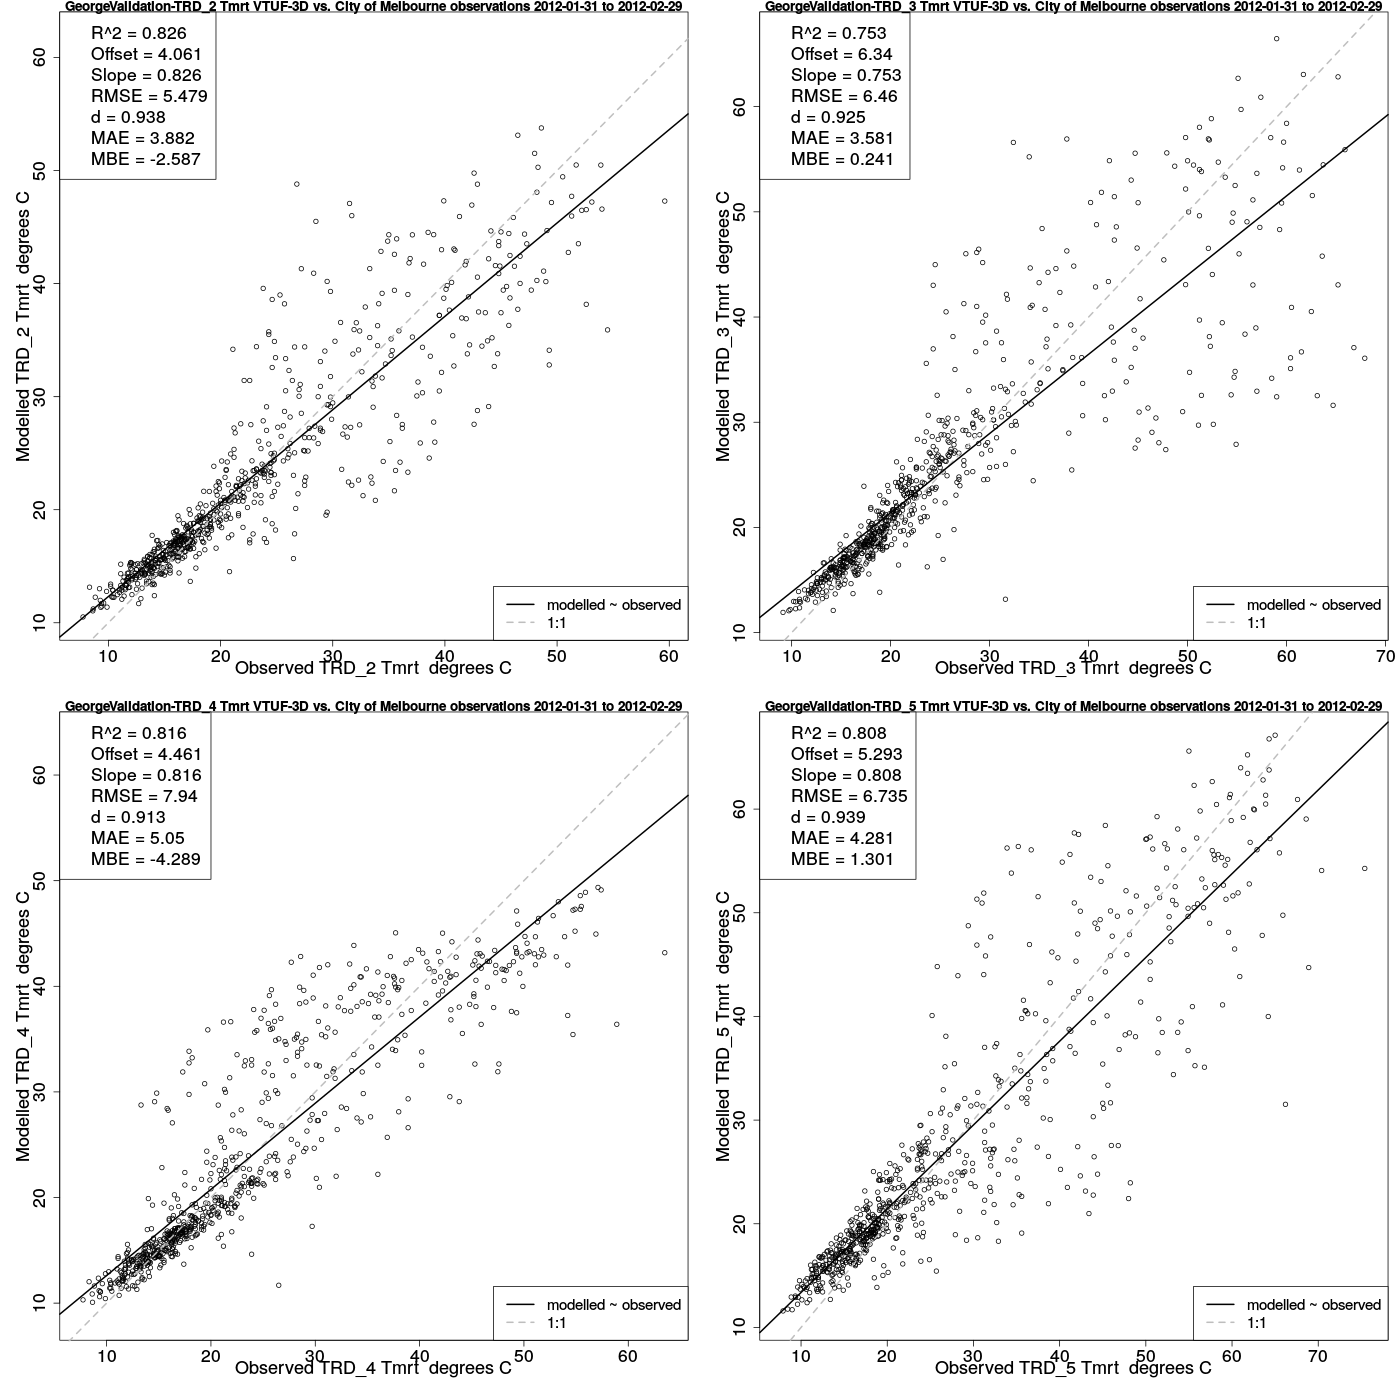
\includegraphics[trim = 0mm 0mm 0mm 0mm, clip, scale=0.30]{images/GeorgeValidation-ErrorPlots-Tmrt7.png}
\caption{George St. GeorgeValidation scenario point comparison of $T_{mrt}$ of 4 observation stations to modelled points.\label{fig:GeorgeStTmrtCompare}} 
\end{figure}

\begin{figure}[!htbp]
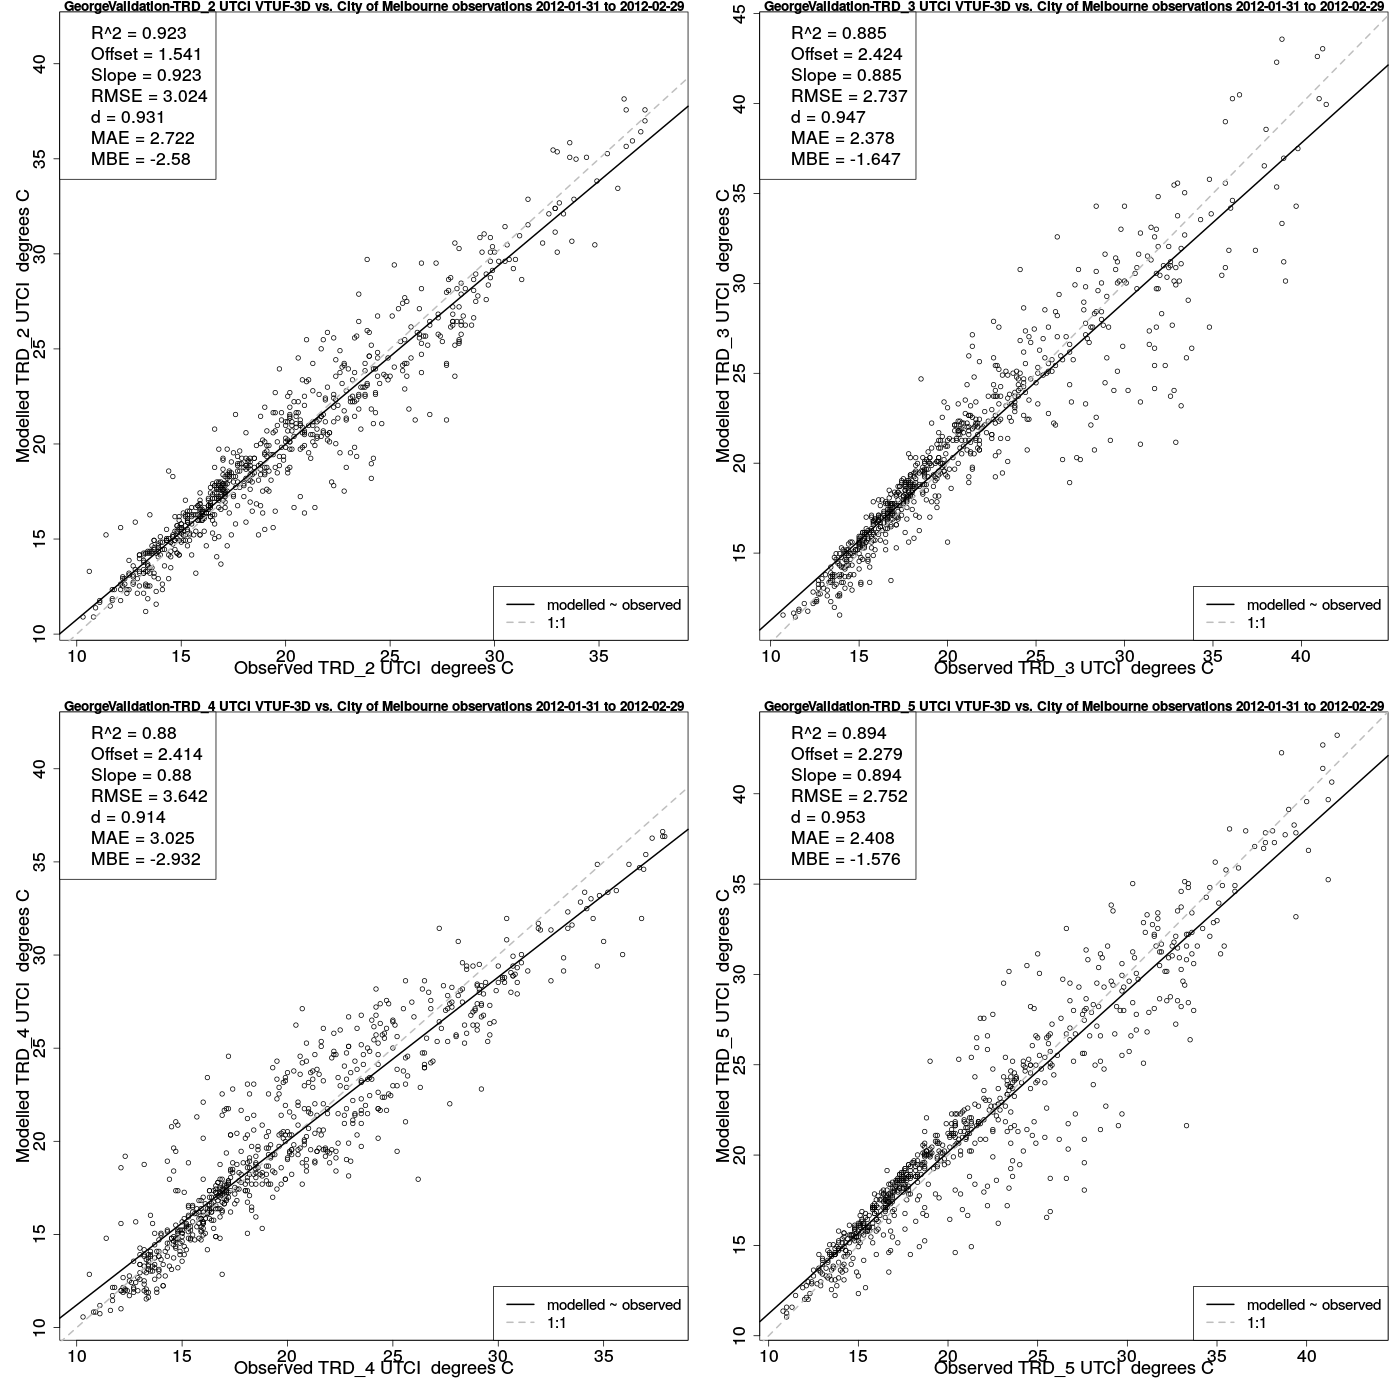
\includegraphics[trim = 0mm 0mm 0mm 0mm, clip, scale=0.30]{images/GeorgeValidation-ErrorPlots-UTCI7.png}
\caption{George St. GeorgeValidation scenario point comparison of UTCI of 4 observation stations to modelled points.\label{fig:GeorgeStUtciCompare}} 
\end{figure}

\begin{figure}[!htbp]
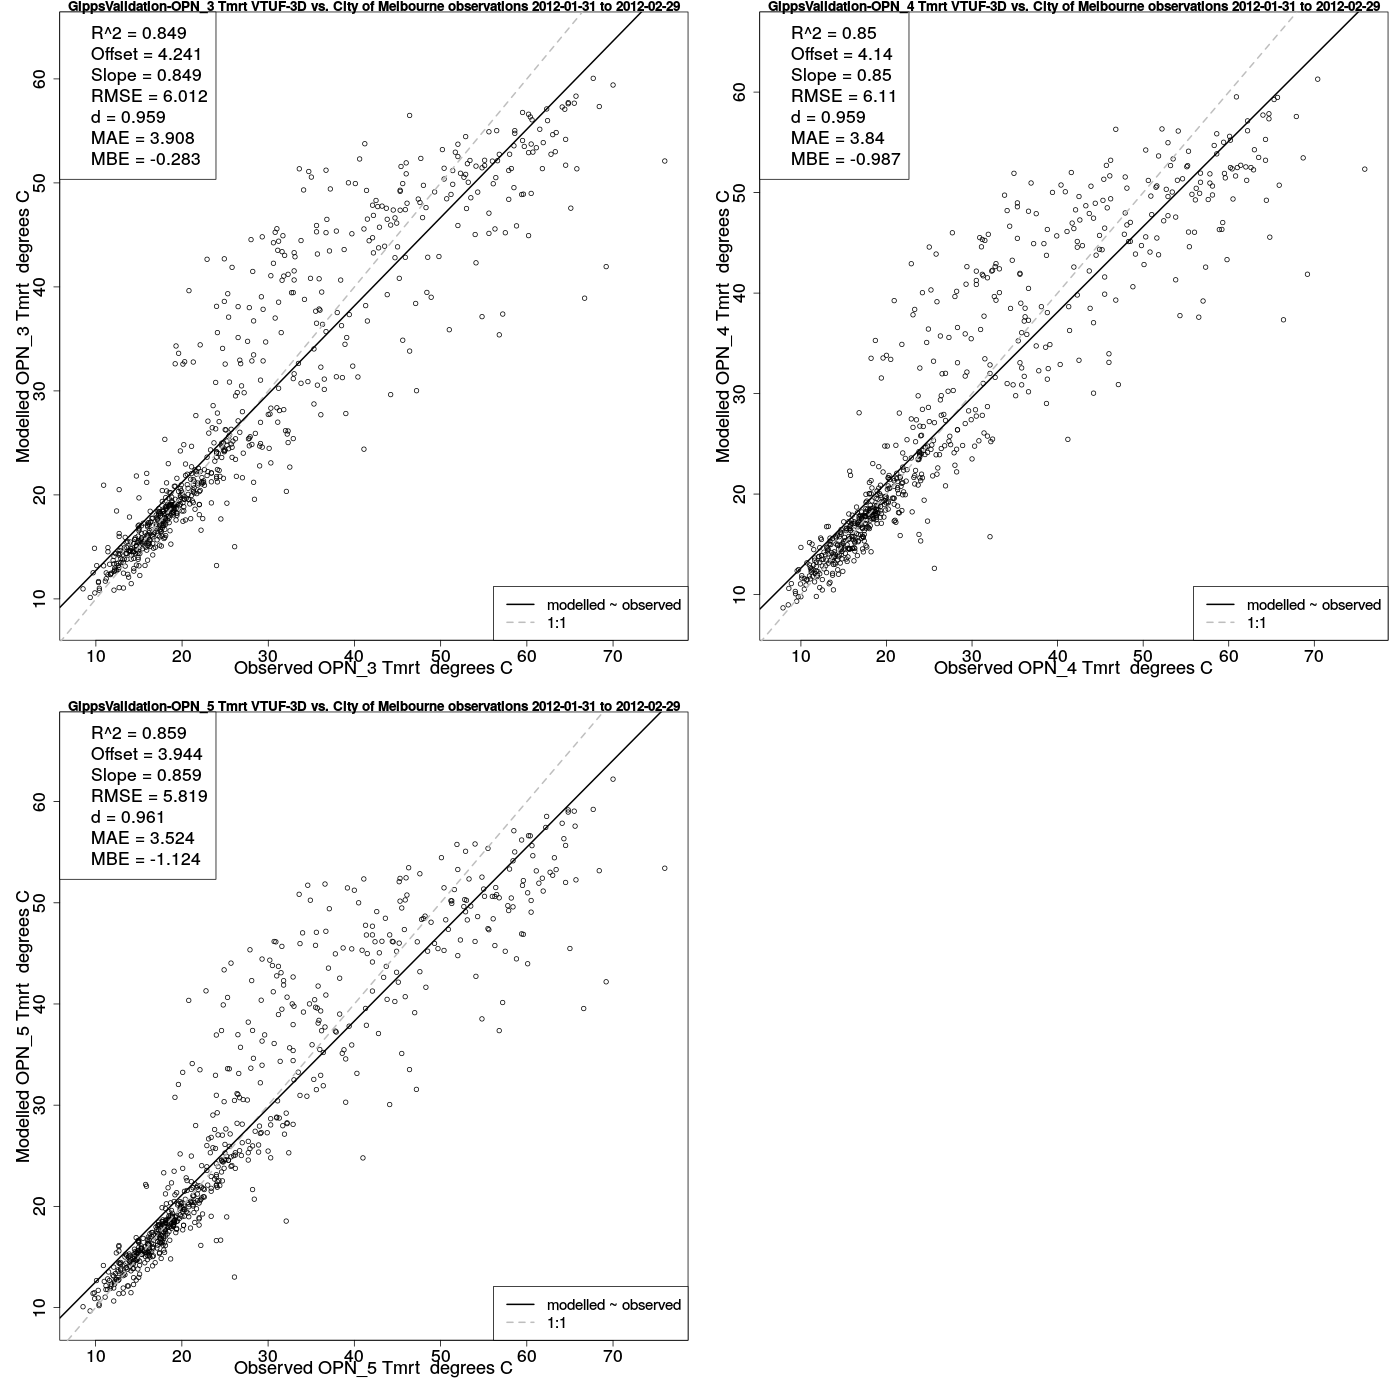
\includegraphics[trim = 0mm 0mm 0mm 0mm, clip, scale=0.30]{images/GippsValidation-ErrorPlots-Tmrt7.png}
\caption{Gipps St. GippValidation scenario point comparison of $T_{mrt}$ of 3 observation stations to modelled points.\label{fig:GippsStTmrtCompare}} 
\end{figure}

\begin{figure}[!htbp]
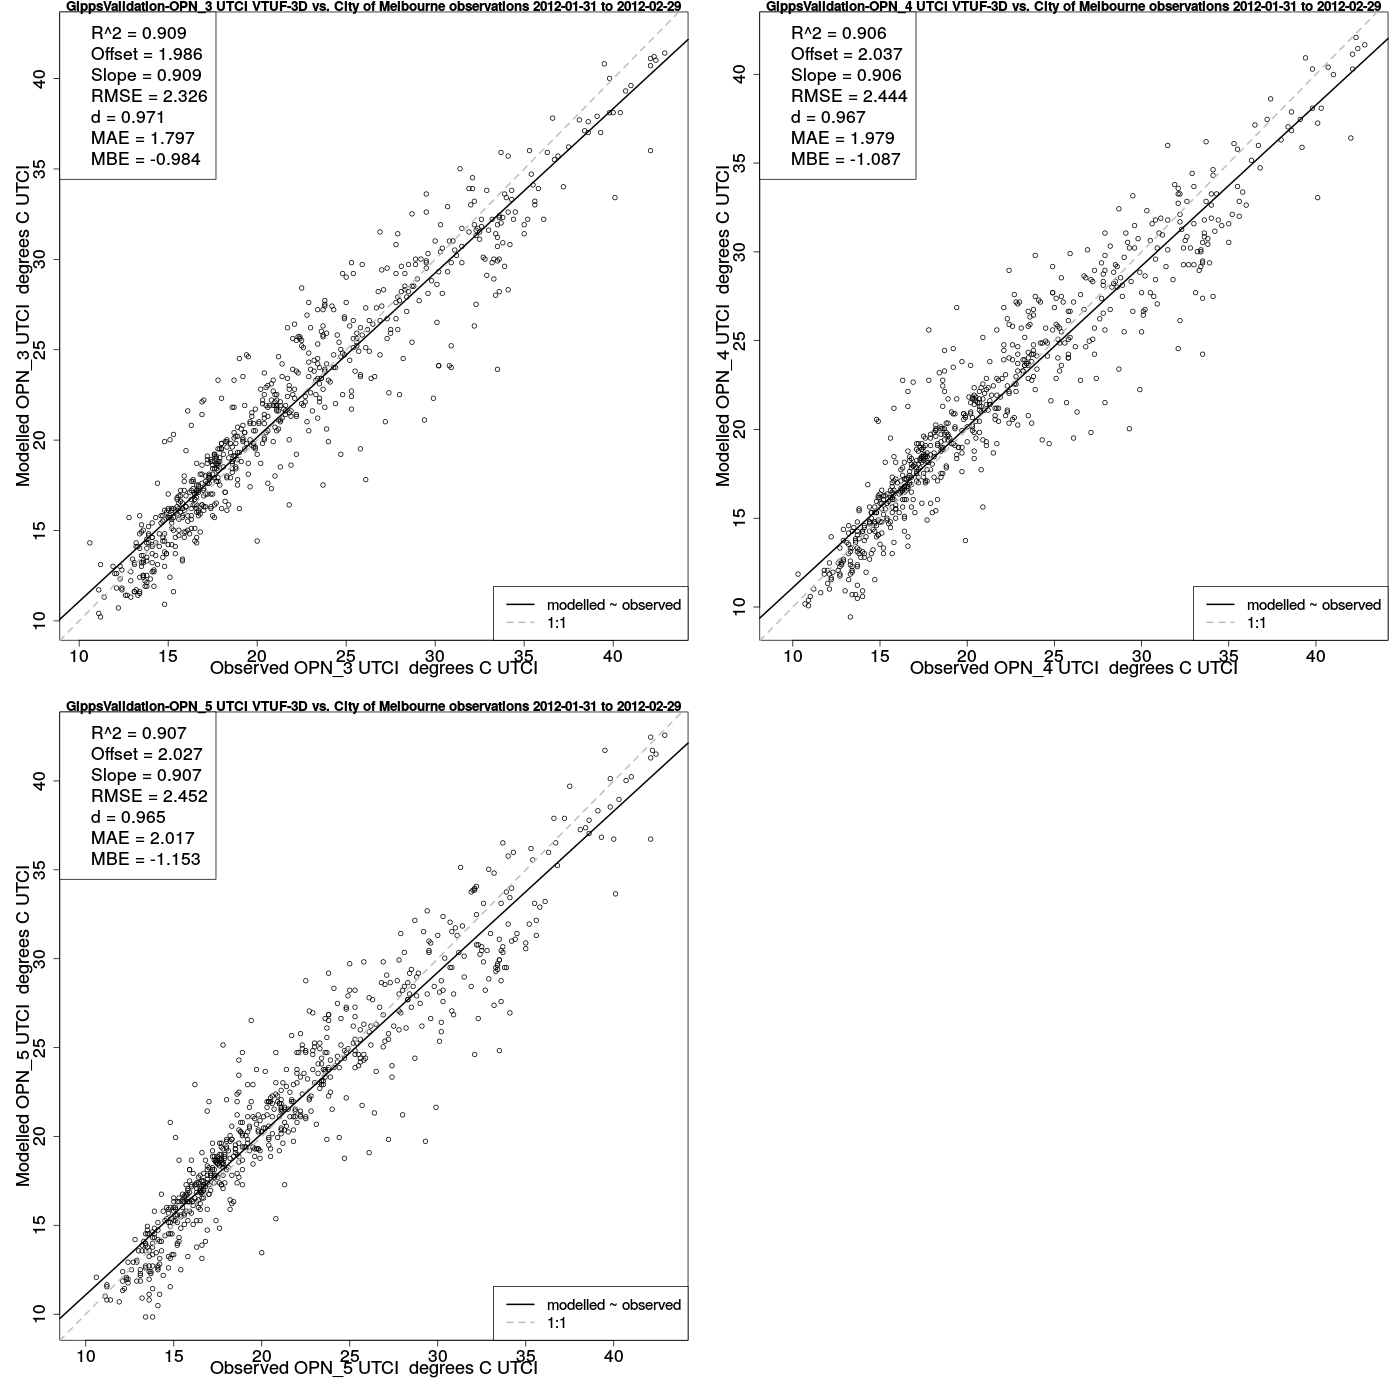
\includegraphics[trim = 0mm 0mm 0mm 0mm, clip, scale=0.30]{images/GippsValidation-ErrorPlots-UTCI7.png}
\caption{Gipps St. GippValidation scenario point comparison of UTCI of 3 observation stations to modelled points.\label{fig:GippsStUtciCompare}} 
\end{figure}


The model shows reasonably good performance in this spatial point by point comparison. $T_{mrt}$ $RMSE$ values from George St. range from 5.48 to 7.94\SI{}{\degreeCelsius}, $T_{mrt}$ $MBE$ values from 0.24 to -4.29\SI{}{\degreeCelsius}, and $d$ index of agreement values range from 0.913 to 0.939. UTCI $RMSE$ values range from 2.74 to 3.02\SI{}{\degreeCelsius}, $T_{mrt}$ $UTCI$ values -1.58 to -2.93\SI{}{\degreeCelsius}, and $d$ index of agreement values range from 0.914 to 0.953.  Gipps St. shows similar results, with $T_{mrt}$ $RMSE$ values ranging from 5.82 to 6.11\SI{}{\degreeCelsius}, $T_{mrt}$ $MBE$ values from -0.28 to -1.12\SI{}{\degreeCelsius}, and $d$ index of agreement values range from 0.959 to 0.961. UTCI $RMSE$ values range from 2.33 to 2.45\SI{}{\degreeCelsius}, $T_{mrt}$ $UTCI$ values from -0.98 to -1.15\SI{}{\degreeCelsius}, and $d$ index of agreement values range from 0.965 to 0.971.

To examine the variations between the different observation points,  the four locations for George St. (TRD\_2, TRD\_3, TRD\_4, and TRD\_5) observations of $T_{mrt}$ were aggregated into hourly averages over 30 days and compared to the same aggregation of the modelled results (Figure \ref{fig:GeorgeSt30Compare}). This same analysis was also performed for the  Gipps St. points (OPN\_3, OPN\_4, and OPN\_5) in Figure \ref{fig:GippsSt30Compare}. For UTCI, a similar analysis for the Gipps St. points (OPN\_3, OPN\_4, and OPN\_5) is presented in Figure \ref{fig:GippsStUTCI30Compare}. 

\begin{figure}[!htbp]
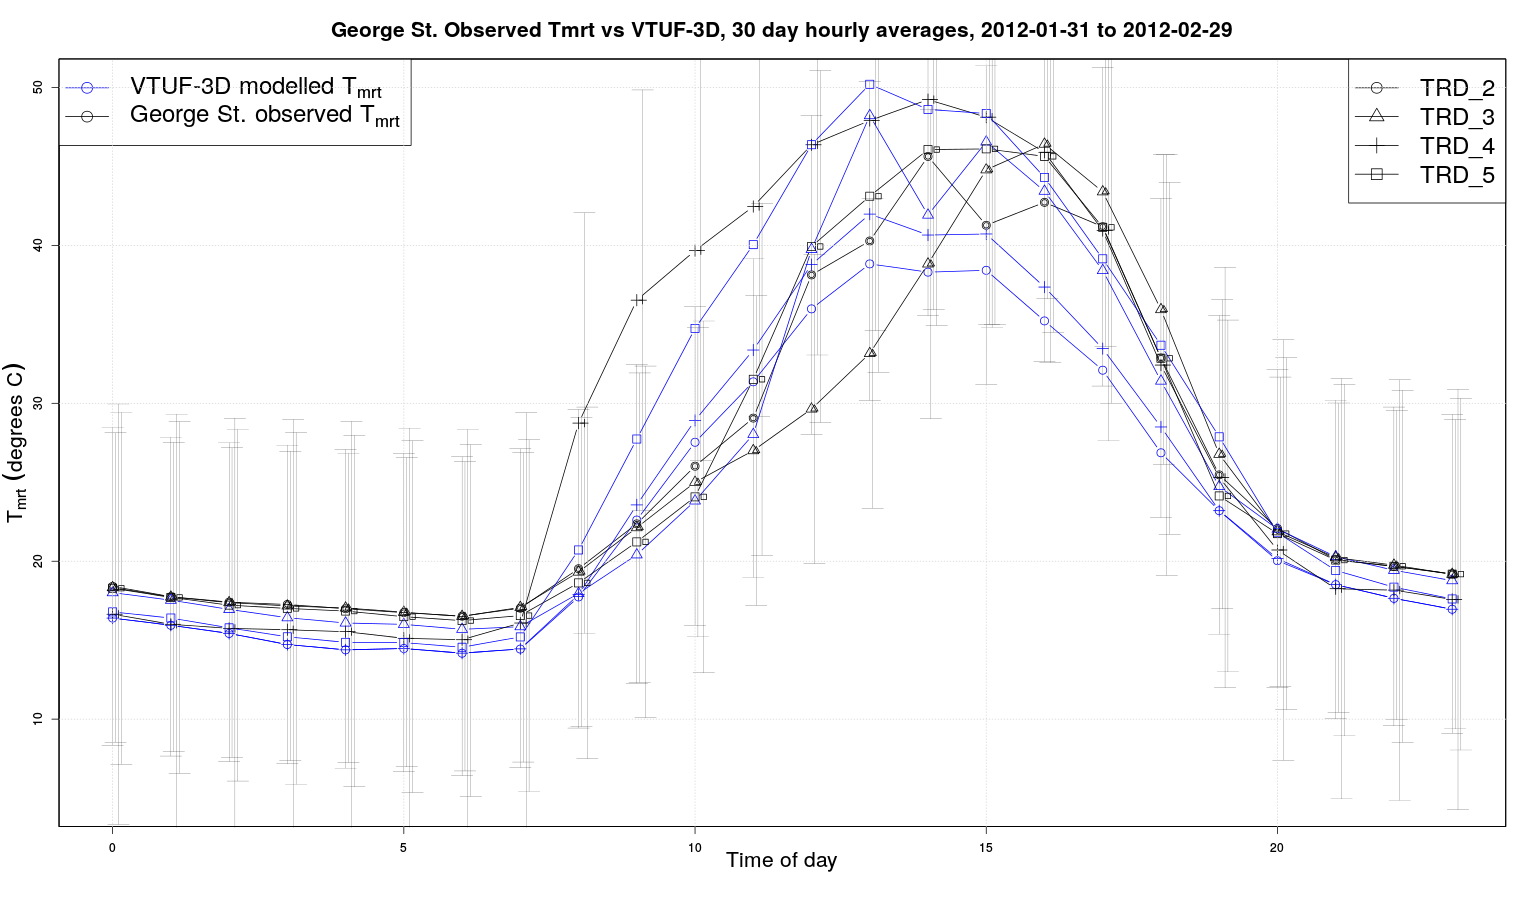
\includegraphics[trim = 0mm 0mm 0mm 0mm, clip, scale=0.32]{images/GeorgeValidationTmrtOverallAve5_.png}
\caption{George St. GeorgeValidation scenario four observation stations (TRD\_2, TRD\_3, TRD\_4, and TRD\_5) values of $T_{mrt}$ aggregated into hourly averages over 30 days compared to modelled points, with error bars at observation standard deviations.\label{fig:GeorgeSt30Compare}} 
\end{figure}

\begin{figure}[!htbp]
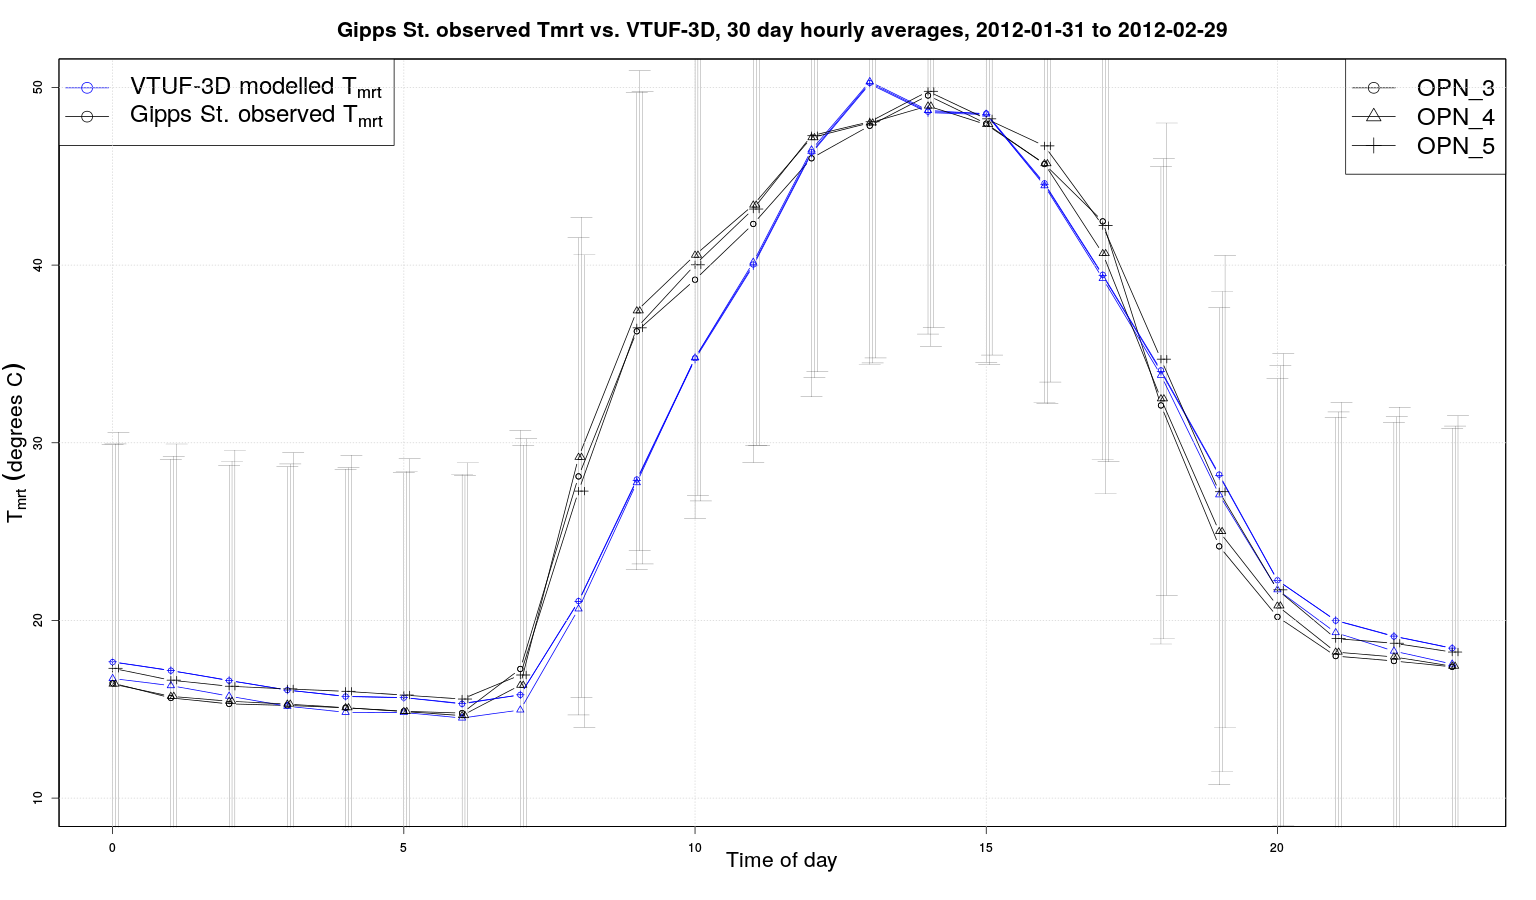
\includegraphics[trim = 0mm 0mm 0mm 0mm, clip, scale=0.32]{images/GippValidationTmrtOverallAve5_.png}
\caption{Gipps St. GippValidation scenario three observation stations (OPN\_3, OPN\_4, and OPN\_5) values of $T_{mrt}$ aggregated into hourly averages over 30 days compared to modelled points, with error bars at observation standard deviations.\label{fig:GippsSt30Compare}}
\end{figure}

\begin{figure}[!htbp]
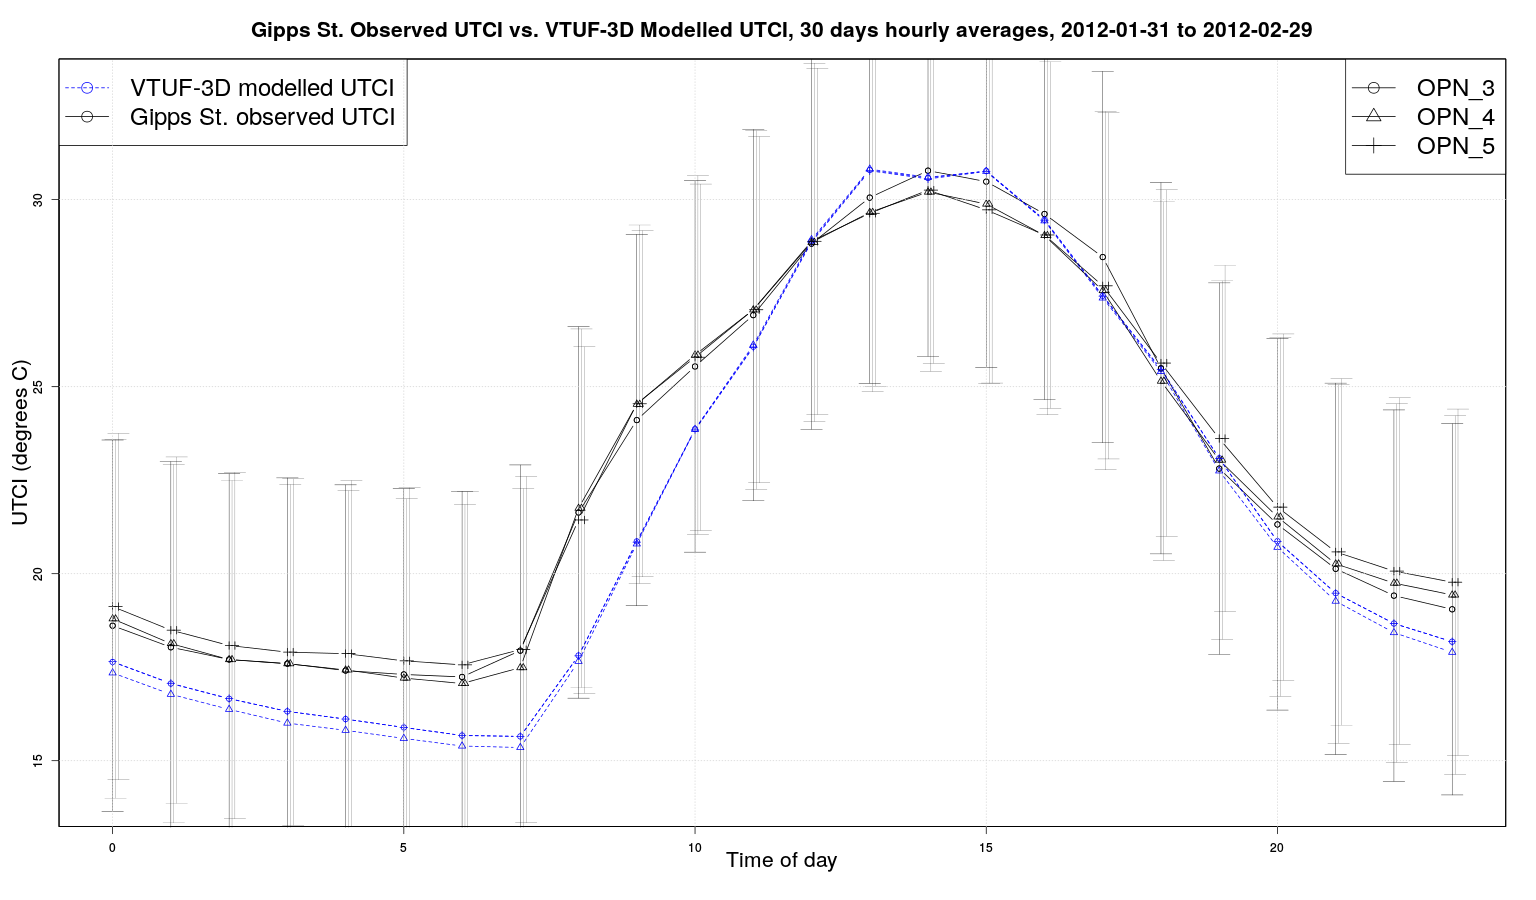
\includegraphics[trim = 0mm 0mm 0mm 0mm, clip, scale=0.32]{images/GippValidationUtciOverallAve5_.png}
\caption{Gipps St. GippValidation scenario three observation stations (OPN\_3, OPN\_4, and OPN\_5) values of UTCI aggregated into hourly averages over 30 days compared to modelled points, with error bars at observation standard deviations.\label{fig:GippsStUTCI30Compare}}
\end{figure}

In the observations, the open canyon of Gipps St. shows very little variation in $T_{mrt}$ across the locations while the treed canyon of George St. shows wide variations, especially between stations TRD\_2 and TRD\_3. TRD\_4, a highly exposed location, shows the highest $T_{mrt}$ values in the late mornings, warming quicker than all the other locations, as well as reaching the highest afternoon peak. TRD\_3 warms the slowest in the mornings, with early morning building shade with continued early afternoon canopy shading. TRD\_2 and TRD\_5 also warm slowly in the mornings due to building shading and vegetation shading respectively and both reach a reduced afternoon peak (compared to TRD\_4).  All observation stations come back into closer agreement in the late afternoons.

The modelled results reproduce the close agreement between the three locations in the open canyon of Gipps St. Variations from the diurnal trends in the observations are seen in slightly slower warming during the mornings but then coming into good agreement at the afternoon peak and throughout the rest of the day and night into the next morning. Very similar patterns are seen in the diurnal trends of UTCI, of which $T_{mrt}$ is the main driver, showing slower warming during the mornings. However, lower modelled UTCI values during the night-time would suggest there is some room for improvement in modelling wind speed or relative humidity, as modelled values of air temperature and $T_{mrt}$ tend to be slightly high and could not be the source of these lower calculated values.

In the treed canyon, George St., the model shows some of the same variation in $T_{mrt}$ between modelled locations seen in the observations. Modelled values of TRD\_4 do reproduce the slower warming trends in the mornings seen in the observations (but diverge in the late mornings). However, the stronger warming of TRD\_4 seen in the observations is not completely captured by the model. In variations from the observed diurnal trends, the modelling results reproduce well the trends from late afternoon, over night, and into early mornings. The main variability during the warming mornings do not show the wide ranges seen in the observations but follow a more average range between those wider ranges. 

There are a number of differences in the way $T_{g}$ (and its use in calculating $T_{mrt}$) (see Section \ref{sec:tmrtutci}) is calculated compared to the observed values, which could explain some of the divergences. First, the modelled results are calculated for each surface in the domain (and only for surfaces in the domain). As there are no surfaces at the locations at which the observations were taken (3.5 to 4m above the ground), the comparisons of $T_{mrt}$ needed to be performed on the modelled results at a 0m height underneath the observation locations. This would lead to lower amounts of $K\downarrow$ reaching the ground due to reduced sky view factors deeper into the urban canyon, especially in the mornings when much of the canyon floor will be in shadow due to lower sun angles.

A second important difference is due to the limitation of domains created using flat cubic surfaces. The globe thermometer in the observation would have been exposed to radiation from all side angles in addition to up and down. As flat surfaces, the modelled points will see a reduction in received shortwave, especially in the mornings. In addition, the lower locations of the points in the canyon will also contribute to lower received shortwave in the same way.


A comparison of modelled $T_{can}$ from scenarios GeorgeValidation and GippValidation to observed $T_{a}$ of George St. 4 treed canopy stations and Gipps St. 3 open canopy stations is shown in Figure \ref{fig:GeorgeGippsStTcanCompare}. Values from both data sets are aggregated into hourly averages over the modelled period. 

A direct comparison of these two data sets is difficult as the modelled $T_{can}$ values are averages of the entire canopy air space while the seven observation stations record the air temperatures at 3.5 to 4m height for each specific location. However, the modelled $T_{can}$ of the open canopy street (Gipps St.) shows peak values approximately 1\SI{}{\degreeCelsius} warmer (as well as being overall warmer throughout daylight hours) than the treed street (George St.). This result is comparable to the \cite{Coutts2015} observations and shows the model is able to capture relative cooling effects of increased canopy cover in air temperature predictions.

\begin{figure}[!htbp]
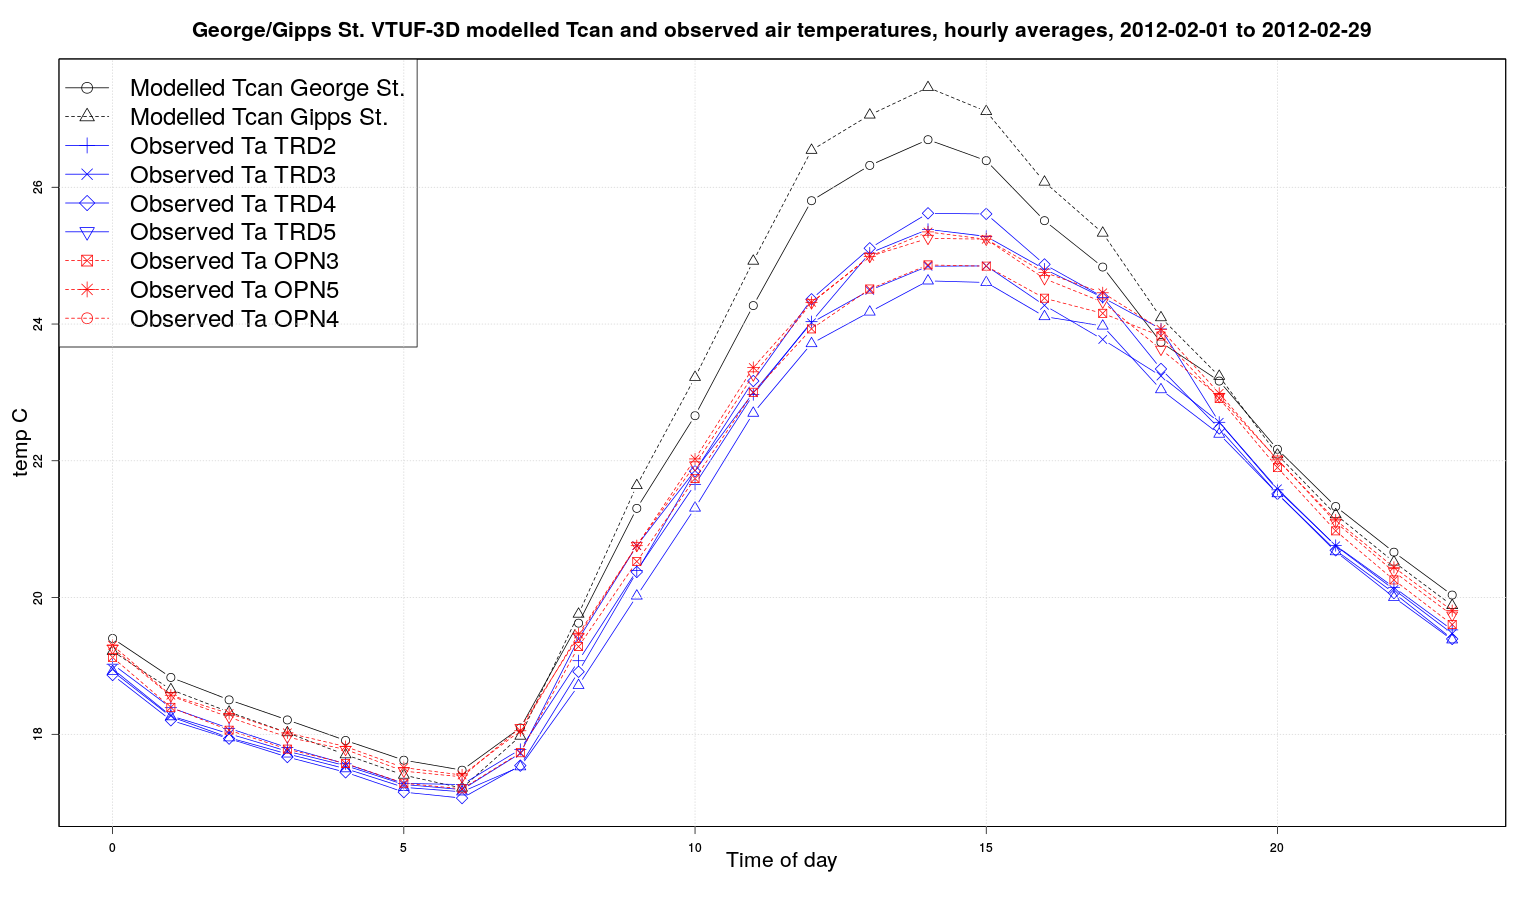
\includegraphics[trim = 0mm 0mm 0mm 0mm, clip, scale=0.30]{images/GeorgeValidationTcanAgg.png}
\caption{George/Gipps St. modelled $T_{can}$ from scenarios GeorgeValidation and GippValidation compared to observed $T_{a}$ of George St. 4 treed canopy stations and Gipps St. 3 open canopy stations, aggregated into hourly averages over February 2012 modelled period.\label{fig:GeorgeGippsStTcanCompare}} 
\end{figure}


\section{Summary and Conclusions}

This study presents the development of a new model, VTUF-3D, that is able to model vegetation and WSUD features, accounting for latent energy fluxes and their impacts on HTC. Two major modifications were made to the original TUF-3D model in the development of VTUF-3D. The first major modification added physical representations of vegetation and allow the shading effects of those features to be modelled. The second major modification added the ability to model vegetation physiological processes (and associated water cycles) and account for latent energy fluxes in surface energy balances.

This analysis of VTUF-3D performance when comparing predicted results to flux tower observations and in comparison to error rates of other urban models has shown significant improvement over the unimproved (non-vegetated) TUF-3D model. Furthermore, these comparisons to observations show the model is able to capture well the temporal and amplitude variations of fluxes observed by flux towers. In a comparison of VTUF-3D modelled results to other types of urban land surface schemes, VTUF-3D performs well within the range of those other models. Significantly, VTUF-3D is able to perform with this level of accuracy at a micro-scale. The majority of the other compared urban models can only deliver local-scaled results at best. Statistical analysis puts VTUF-3D's performance in all fluxes, except $Q_{E}$, as slightly better than all categories of these models. With the $Q_{E}$ flux, VTUF-3D performs with lower error rates than the models in the no vegetation category but with slightly higher errors than in the tiled and integrated categories. This evaluation demonstrates that VTUF-3D performs well in terms of surface energy balances, lending weight to its suitability to assess the impacts of urban greenery on human thermal comfort.

Observations of two contrasting street canyons with varying amounts of canopy cover were used to further evaluate the model's performance and test VTUF-3D's ability to predict values of $T_{mrt}$ and UTCI, both spatially and temporally. $RMSE$ and $d$ index of agreement values when comparing the modelled results of both variables to point observations show reasonably good performance of the model. In reproducing diurnal trends of $T_{mrt}$, VTUF-3D is able to reproduce the overall trends well except is slightly slow to warm during the mornings. In the treed canyon of George St., where wide variations between the observation stations are seen in the observations, VTUF-3D is able to reproduce much of those variations but not the entire range. This indicates that there is still room for improvement in the specific modelling of vegetation in urban canyons and resolving the $T_{mrt}$ values. The completion of this evaluation shows that VTUF-3D is able to successfully predict values of $T_{mrt}$ and UTCI across a variety of urban canyons.

VTUF-3D is a unique model involving an innovative tiling approach that accounts for the detailed physiological processes of vegetation. The model incorporates a templated scalable configuration system, used to represent specific types of vegetation, allowing any variety and mix of vegetation to be added to a modelled domain. Also, differential shading functionality allows impacts of urban geometry and inter-tree shading on vegetation anywhere in an urban canyon to be properly modelled. Finally, the addition of mean radiant temperature and UTCI output for all surfaces allows detailed analysis of the impact of vegetation on these important parameters influencing HTC in these areas.

An extensive evaluation process has shown that VTUF-3D is able to accurately model urban areas (including urban vegetation). Now, with the completion and evaluation of the VTUF-3D v1.0 model, there is a suitable tool to model and study in detail the impacts of urban greening on HTC and recommendations and guidelines on how best to best use urban greenery to reduce urban temperatures. Questions can be answered as to the optimal arrangement of canopy cover to give the maximum benefits. Performance of future scenarios can also help inform responses to future challenges, both in terms of urban redesign and understanding how current urban design will respond to changing urban climate conditions.

With VTUF-3D's micro-climate resolution, urban areas can be studied metre by metre and proper mitigation strategies designed for every section of the urban canyon, allowing effort to be focused on areas with the greatest need. VTUF-3D is sufficiently scaled to resolve human level interactions with their surroundings and provide variables to calculate HTC (such as T$_{mrt}$). The built in output of T$_{mrt}$ and UTCI allows examination of these values without requiring addition steps. Finally, with the ability to insert any type of vegetation using physiological and physical vegetation templates, VTUF-3D is applicable to an unlimited number of scenarios and modelling questions. This new model will allow research into a wide variety of urban morphologies, quantifying the benefits of a wide variety of urban arrangements and allow planning for future changes and challenges in climate and urban design.

However, the creation and evaluation of VTUF-3D is only a first step. As the intended end users of the knowledge gained through VTUF-3D, planners and policy makers, often lack the time, expertise, and scientific rigour needed to generate and interpret climate model output \citep{Elasson2000,Moser2014,Winkler2011}, additional work will need to be done with VTUF-3D to systematically analyse a wide variety of scenarios seeking optimal uses of urban vegetation for HTC and summarise these findings. A forthcoming article will start this process with an examination by VTUF-3D of varying urban canopy cover on HTC in street canyons. VTUF-3D has also been adopted by the CRC for Water Sensitive Cities as their micro-climate tool to evaluate climatic impacts of WSUD, with those findings disseminated to industry partners and the public at large. Finally, work is under way to provide a simpler user interface to VTUF-3D, allowing a wider adoption beyond the current academic research user-base.



\section{Code availability}\label{sec:available}

Development of VTUF-3D was conducted in FORTRAN 2003 \citep{GNU2016a} in Netbeans 8.0.2 \citep{Netbeans2016} and compiled with gfortran 4.8.4 \citep{GNU2016} on Ubuntu 14.04, however, the code should compile on any platform with FORTRAN 2003 support. The original source code for TUF-3D was obtained from the author \citep{Krayenhoff2007}, while source code for MAESPA was obtained from the MAESPA repository \citep{Duursma2016}. The development process merged these code bases and added the additional functionality described in this paper. The VTUF-3D source code is available at \cite{Nice2016c}.

Model configuration process was developed in Java using the JRE 1.7.0 \citep{Oracle2016} in Eclipse 4.5.2 \citep{Eclipse2016}. Data analysis and graphing scripts were generated in R \citep{R2013} and Python \citep{Python2016} using the Matplotlib library \citep{Hunter2007}. 

\section*{Acknowledgements}
The support of the Commonwealth of Australia through the Cooperative Research Centre program is acknowledged.
%\end{acknowledgements}

\section*{References}\label{sec:ref}
%% If you have bibdatabase file and want bibtex to generate the
%% bibitems, please use
%%
  \bibliographystyle{elsarticle-harv} 
  \bibliography{library}

%% else use the following coding to input the bibitems directly in the
%% TeX file.

\begin{thebibliography}{00}

%% \bibitem[Author(year)]{label}
%% Text of bibliographic item

\bibitem[ ()]{}

\end{thebibliography}


%% The Appendices part is started with the command \appendix;
%% appendix sections are then done as normal sections
\appendix
\setcounter{table}{0}
\renewcommand{\thetable}{A\arabic{table}}

%\subsection{}                               %% Appendix A1, A2, etc.


%%%%%%%%%% taking out parameterizations
\section{MAESPA vegetation parameterisations}\label{sec:maespavegpara}  
%

The first complete parameterisation for VTUF-3D is the olive tree (\textit{Olea europaea}). It has been selected because it is a species commonly found in gardens in Melbourne, considered suitable for Melbourne's climate conditions (drought tolerant evergreen), and are a recommended species for council street tree planting \citep{PortPhillip2010}. In addition, observations of parameters are available from \cite{Coutts2014a}. The physical and meteorological parameters for a 5x5 meter grid square are given in Table \ref{tab:olivescaled}. Physiology parameter values are shown in Table \ref{tab:oliveparam}. The second complete parameterisation for VTUF-3D is the  brushbox tree (\textit{Lophostemon Confertus}). This tree is chosen because it is the most common street tree in Melbourne \citep{Frank2006}, where all of the evaluation observations data sets are based. This tree has also been the basis of a number of research projects in Melbourne, providing a parameterisation through \cite{Coutts2016} and \cite{Coutts2015ICUC}. The third complete parameterisation for VTUF-3D is for grass, tall fescue (\textit{Festuca arundinacea}), a common turf grass. This is an important parameterisation for modelling urban environments as a significant portion of urban surfaces are grass. As will be seen in the VTUF-3D evaluation (forthcoming paper), estimates of observed grass cover, for example in an evaluation based on observations from Preston in Melbourne \citep{Coutts2007,Nury2015}, range from 11\% to 23\%. 

This parameterisation is an adaptation of the normal MAESPA tree parameterisations. In it, the vegetation is modelled as a box shaped canopy with a crown height of 0.2 meters. The 0.2 value was taken from the literature, and represents the blade length of the grass. While the crown height for grass is set to 0.2m, in reality, lawn grass does not grow perfectly perpendicular to the ground, so the blade length is actually longer than perceived. In addition, not all urban lawns are well maintained and closely manicured. Further, while grass is accounted for in the model, though may be slightly overestimated, other vegetation such as shrubs were not accounted for, so in any event, the long grass blade length accounts for some effects of not accounting for shrubs and other urban understory items. This and the rest of the physical and meteorological parameters for a 5x5 meter grid square are given in Table \ref{tab:olivescaled}, with physiology parameter values (Table \ref{tab:oliveparam}) taken from the literature.

\begin{center}
\begin{table}[!htbp]
\caption{MAESPA parameterisations of structural characteristics for \textit{Olea europaea}, \textit{Lophostemon Confertus}, and \textit{Festuca arundinacea}, tree dimensions for an example 5x5m grid (that are rescaled for taller/shorter modelled trees).\label{tab:olivescaled}}
\begin{tabular}{ |  p{2.5cm} | p{1.1cm} | p{2.5cm} | p{1.1cm} | p{2.5cm} | p{1.1cm} | p{2.5cm} | }

\hline & \multicolumn{2}{|c|}{\textit{Olea europaea}} & \multicolumn{2}{|c|}{\textit{Lophostemon Confertus}} &\multicolumn{2}{|c|}{\textit{Festuca arundinacea}}   \\ \hline

\hline \textbf{Parameter} & \textbf{Value} & \textbf{Source} & \textbf{Value} & \textbf{Source}& \textbf{Value} & \textbf{Source} \\ 
\hline
crown radius (m) & 2.5 & \cite{Coutts2014a}  & 2.5 &\cite{Coutts2016} & 2.5& Radius of 5x5m grid  \\ \hline
crown height (m) & 3.75 & \cite{Coutts2014a}  & 3.75&\cite{Coutts2016} & 0.2& \cite{Simmons2011}  \\ \hline
trunk height (m) & 1.25 & \cite{Coutts2014a}  & 1.25&\cite{Coutts2016} & 0.01&  \\ \hline
leaf area index (m$^{2}$ m$^{-2}$)&2.48 &\cite{Mariscal2000}  &2.0&\cite{Wright2000} &  7.13 & ave. from \cite{Bijoor2014} \\ \hline
crown shape & round &  & round & & box&  \\ \hline
$z_{Ht}$ (m)&40.0&Forcing data height   &4.0&Forcing data height &4.0&Forcing data height \\ \hline
$z_{PD}$ (m) &2.5& 2/3 of crown height \citep{Grimmond1999}  &2.5 & 2/3 of crown height \citep{Grimmond1999} &0.066 & 2/3 of crown height \citep{Grimmond1999} \\ \hline
$z_{0,Ht}$ (m) &0.375& 1/10 of crown height \citep{Grimmond1999}  &0.375 & 1/10 of crown height \citep{Grimmond1999}  & 0.02 & 1/10 of crown height \citep{Grimmond1999}  \\ \hline
\end{tabular} 
\end{table}
\end{center}


\begin{center}
\begin{table}[!htbp]
\caption{MAESPA parameterisations of species physiology for \textit{Olea europaea}, \textit{Lophostemon Confertus}, and \textit{Festuca arundinacea}, with parameter values taken from cited literature sources. \label{tab:oliveparam}}

\scalebox{1.00}{
\begin{tabular}{ |  p{3.5cm} | p{1.1cm} | p{2.5cm} | p{1.1cm} | p{2.5cm} | p{1.1cm} | p{2.5cm} | }
\hline & \multicolumn{2}{|c|}{\textit{Olea europaea}} & \multicolumn{2}{|c|}{\textit{Lophostemon Confertus}} &\multicolumn{2}{|c|}{\textit{Festuca arundinacea}}   \\ 
\hline \textbf{Parameter} & \textbf{Value(s)} & \textbf{Source}& \textbf{Value(s)} & \textbf{Source}& \textbf{Value(s)} & \textbf{Source} \\ 
\hline
Soil reflectance (\%PAR, \%NIR, and \%IR)  & 0.10, 0.05, 0.05 & \cite{Levinson2007,Oke1987z} & 0.04, 0.35, 0.05 & \cite{Fung-yan1999}&0.10, 0.05, 0.05&  Observed, \cite{Levinson2007}, \cite{Oke1987z}  \\ \hline
Leaf transmittance (\%PAR, \%NIR, and \%IR)  & 0.01, 0.28, 0.01 & \cite{Baldini1997} &&& 0.05, 0.45, 0.01 & C3 grasses, from \cite{Katjacnik2014}\\ \hline
Leaf reflectance (\%PAR, \%NIR, and \%IR)  & 0.08, 0.42, 0.05 & \cite{Baldini1997} &&& 0.05, 0.65, 0.08  & C3 grasses, from \cite{Katjacnik2014} \\ \hline
Minimum stomatal conductance g0 (mol m$^{-2}$s$^{-1}$) & 0.03 & \cite{Coutts2014a} & 0.01 & \cite{Coutts2016}& 0.0 &  \cite{DeKauwe2015}\\ \hline
Slope parameter g1  & 2.615 &\cite{Coutts2014a} &3.33&\cite{Coutts2016}&5.25& C3 grasses, from \cite{DeKauwe2015}\\ \hline
\# of sides of the leaf with Stomata & 1&\cite{Fernandez1997}  & 1&\cite{Beardsell1987}& 2& \cite{Green1990}\\ \hline
Width of leaf (m)& 0.0102& &  0.05&\cite{Coutts2016}& 0.006& \cite{RademacherI2001}\\ \hline
CO$_{2}$ compensation point ($\mu$mol m$^{-2}$s$^{-1}$)& 55& \cite{Coutts2014a}  & 53.06&\cite{Coutts2016}& 57& \cite{Brown1980} at 25 degrees\\ \hline
Max rate electron transport (Jmax) ($\mu$mol m$^{-2}$s$^{-1}$)& 112.4& \cite{Coutts2014a}  &105.76& \cite{Coutts2016}&80.95& Tall Fescue from \cite{Yu2012a}\\ \hline
Max rate rubisco activity (VCmax) ($\mu$mol m$^{-2}$s$^{-1}$)& 81.18& \cite{Coutts2014a}  & 81.6&\cite{Coutts2016}& 36.14& Tall Fescue from \cite{Yu2012a}\\ \hline
Curvature of the light response curve &0.62& \cite{Coutts2014a}   &0.61 &\cite{Coutts2016}&0.7 &\cite{Gilmanov2007}\\ \hline
Activation energy of Jmax (KJ mol$^{-1}$)& 35350& \cite{Diaz-Espejo2006}  & 35350& \cite{Bernacchi2001}& 65300& \cite{Bernacchi2001}\\ \hline
Deactivation energy of Jmax (J mol$^{-1}$)& 200000 &\cite{Medlyn2005a}  & 200000& \cite{Medlyn2005a}& 200000& \cite{Medlyn2005a}\\ \hline
Entropy term (KJ mol$^{-1}$)& 644.4338& \cite{Medlyn2005a}   & 644.4338& \cite{Medlyn2005a}& 644.4338& \cite{Medlyn2005a}\\ \hline
Quantum yield of electron transport (mol electrons mol$^{-1}$)& 0.19& \cite{Sierra2012}  &0.06&\cite{Coutts2016}&0.05& \cite{Monson1982}\\ \hline
Dark respiration ($\mu$mol m$^{-2}$s$^{-1}$)& 0.94& \cite{Coutts2014a}  &1.29 &\cite{Coutts2016}&0.6  & Estimated for Tall Fescue from \cite{Yu2012a}\\ \hline
Specific leaf area (mm$^{2}$kg$^{-1}$)&5.1 &\cite{Mariscal2000}  &25.3 &\cite{Wright2000}&23.16 &Average from Table 1 in \cite{Bijoor2014} for 3 turfgrasses.\\ \hline
\end{tabular} 
}
\end{table}
\end{center}




%\authorcontribution{This work was developed by Kerry Nice and supervised by Andrew Coutts and Nigel Tapper. Model source code was received from Scott Krayenhoff and Remko Duursma (as acknowledged in Section \ref{sec:available}). Synthesis of this code and new code was developed by Kerry Nice. The article was written by Kerry Nice with editing and suggestions from Andrew Coutts and Nigel Tapper.}
%
%\begin{acknowledgements}
%The work described in this paper was developed during a PhD. project at Monash University. Funding for this was obtailed through the City of Melbourne, Monash University, and the CRC for Water Sensitive Cities.  
%\end{acknowledgements}

%\begin{acknowledgements}
%The support of the Commonwealth of Australia through the Cooperative Research Centre program is acknowledged.
%\end{acknowledgements}

%%%% \section{}
%%%% \label{}
%%\section{References}\label{sec:ref}
%%%% If you have bibdatabase file and want bibtex to generate the
%%%% bibitems, please use
%%%%
%%  \bibliographystyle{elsarticle-harv} 
%%  \bibliography{library}
%%
%%%% else use the following coding to input the bibitems directly in the
%%%% TeX file.
%%
%%\begin{thebibliography}{00}
%%
%%%% \bibitem[Author(year)]{label}
%%%% Text of bibliographic item
%%
%%\bibitem[ ()]{}
%%
%%\end{thebibliography}
%%
%%
%%
%%
%%









\end{document}

\endinput
%%
%% End of file `elsarticle-template-harv.tex'.
